\documentclass[10pt]{article}
% Layout of a NeurIPS/ICML submission: single column, 10pt Times, 5.5in x 9in text block.
% Swapping in a venue's style file is a one-line change.
\usepackage[letterpaper,textwidth=5.5in,textheight=9in,top=1in,headsep=0pt,headheight=0pt,footskip=30pt]{geometry}
\usepackage[T1]{fontenc}
\usepackage{times}
\usepackage{microtype}
\usepackage{amsmath,amssymb,amsthm,mathtools}
\usepackage{thm-restate}
\usepackage{booktabs,array}
\usepackage{placeins}
\usepackage{graphicx}
\usepackage[font=small,labelfont=bf]{caption}
\usepackage{tikz}
\usepackage{framed}
\usepackage{needspace}
\usetikzlibrary{positioning,arrows.meta,calc,matrix,fit}
\usepackage[round,sort]{natbib}
\renewcommand{\bibfont}{\small\raggedright}
\renewcommand{\bibsection}{\section*{References}\addcontentsline{toc}{section}{References}}
\usepackage[colorlinks,linkcolor=blue!45!black,citecolor=blue!45!black,urlcolor=blue!45!black]{hyperref}
\usepackage[capitalise,noabbrev,nameinlink]{cleveref}
\usepackage{enumitem}
\setlist{nosep,leftmargin=1.4em}
\setlength{\textfloatsep}{10pt plus 2pt minus 2pt}
\renewcommand{\topfraction}{0.85}
\renewcommand{\textfraction}{0.1}

% TeX Live 2026 (LaTeX 2026-06-01) makes a theorem that shares a counter an alias of it (\newcounteralias),
% and thmtools, loaded by thm-restate, would make the same alias again, an error. Leave the alias to LaTeX;
% on older TeX Live, without \newcounteralias, nothing changes.
\makeatletter
\@ifundefined{newcounteralias}{}{%
  \renewcommand\thmt@autorefsetup{\@xa\def\csname\thmt@envname autorefname\@xa\endcsname\@xa{\thmt@thmname}}%
}
\makeatother
\newtheorem{theorem}{Theorem}[section]
\newtheorem{proposition}[theorem]{Proposition}
\newtheorem{corollary}[theorem]{Corollary}
\newtheorem{lemma}[theorem]{Lemma}
\newtheorem{conjecture}{Conjecture}
\theoremstyle{definition}
\newtheorem{definition}[theorem]{Definition}
\newtheorem*{definition*}{Definition}
\newtheorem{example}[theorem]{Example}
\newtheorem*{example*}{Example}
\theoremstyle{remark}
\newtheorem{remark}[theorem]{Remark}
\newtheorem*{remark*}{Remark}
\crefname{equation}{}{}
\crefname{conjecture}{Conjecture}{Conjectures}
\Crefname{conjecture}{Conjecture}{Conjectures}

\newcommand{\R}{\mathbb{R}}
\newcommand{\Wread}{W_{\mathrm{read}}}
\newcommand{\Wwrite}{W_{\mathrm{write}}}
\newcommand{\dm}{d_{\mathrm{model}}}
\newcommand{\dhid}{d_{\mathrm{hidden}}}
\newcommand{\GL}{\mathrm{GL}}
\newcommand{\Ort}{\mathrm{O}}
\newcommand{\CO}{\mathrm{CO}}
\newcommand{\Aff}{\mathrm{Aff}}
% The Frechet derivative, upright to set it apart from the readout D.
\newcommand{\Der}{\mathrm{D}}
\newcommand{\G}{\mathcal{G}}
\newcommand{\norm}[1]{\lVert #1\rVert}
\newcommand{\para}[1]{\smallskip\noindent\textbf{#1}\hspace{0.5em}}
% The one-sentence summary at the start of a main section.
\newcommand{\takeaway}[1]{\noindent\textit{#1}\par\smallskip}
% A link from a result in the main text to its proof in Appendix A.
% A link target at a part of a statement, and references that link name, number and part to it.
\newcommand{\ptlabel}[1]{\phantomsection\label{#1}}
\DeclareRobustCommand{\cpref}[2]{\hyperref[#1:#2]{\cref*{#1}(#2)}}
\DeclareRobustCommand{\Cpref}[2]{\hyperref[#1:#2]{\Cref*{#1}(#2)}}
\DeclareRobustCommand{\rpref}[2]{\hyperref[#1:#2]{\ref*{#1}(#2)}}
\DeclareRobustCommand{\ptlink}[2]{\hyperref[#1:#2]{(#2)}}
% No page break between a statement and the line that follows it (its "Proof in" line, or its proof).
\makeatletter
\@ifundefined{AddToHook}{}{\AddToHook{env/restatable/begin}{\@endparpenalty\@M}}
\makeatother
\newcommand{\proofin}[1]{\par\vspace{-0.4\baselineskip}\noindent\hfill{\small\itshape Proof in \cref{#1}.}\par\smallskip}
% A main-text result that is a special case of, or follows from, a result in the appendix.
\newcommand{\specialof}[2]{\par\vspace{-0.4\baselineskip}\noindent\hfill{\small\itshape A special case of \cref{#1}, proved in \cref{#2}.}\par\smallskip}
\newcommand{\followsfrom}[2]{\par\vspace{-0.4\baselineskip}\noindent\hfill{\small\itshape Follows from \cref{#1}, proved in \cref{#2}.}\par\smallskip}
% A part of a statement: a link target (if a label is given), a bold number in parentheses and an optional bold name.
\newcommand{\stpart}[3]{\ifx\relax#1\relax\else\ptlabel{#1:#2}\fi{\upshape\bfseries\boldmath(#2)\ifx\relax#3\relax\else\ #3.\fi}}
% A lemma and its proof inside another proof: indented, with a thin gray rule on the left.
\newenvironment{nested}{\par\nopagebreak\def\FrameCommand{\hspace{0.5em}{\color{black!30}\vrule width 0.6pt}\hspace{1em}}\MakeFramed{\advance\hsize-\width\FrameRestore}}{\endMakeFramed}


\title{\Large\bfseries On the Functional Dimension of a Family of\\ Analytic Neural Networks}

\newif\ifanon \anonfalse
\ifanon
\author{Anonymous author}
\else
\author{Marko Karbevski\\
Independent researcher\\
{\small\texttt{markokarbevski@insimplicity.tech}}}
\fi
\date{}

\begin{document}
\maketitle
\vspace{-1.5em}

\begin{abstract}
The functional dimension of a neural network is the number of independent directions in which its parameters change the function that it computes. Symmetries of the parameters bound it from above, and for ReLU networks the bound can fail. We study deep networks in which every layer has input weights, a fixed nonlinear map and output weights, as the layers of a transformer have. Between two such layers, the output weights of the first can be multiplied by an invertible matrix and the input weights of the second by its inverse: a $\GL(\dm)$ symmetry at every hidden state, and an $\Ort(\dm)$ symmetry under pre-RMSNorm. With this symmetry we remove $\dm^2$ (resp. $\approx \dm^2/2$ under pre-RMSNorm) parameters per layer without changing the network function. This is a lossless reduction of about $8.5$ percent of the parameters of the skipless ViT-B of \citet{ji2026cutting}. We then prove that for $\tanh$, SwiGLU and GeGLU layers, and for GELU layers under pre-RMSNorm, nothing more can be removed, at any depth: these symmetries, together with those inside the layers, are the only redundancy, and the networks are locally identifiable up to them.
\end{abstract}

\section{Introduction}\label{sec:intro}

Which parameters of a neural network does the function that it computes determine? For $\tanh$ networks the answer is classical: the function determines the weights up to permutations and sign flips of the hidden units, for irreducible networks with one hidden layer \citep{sussmann1992} and, under conditions that almost all weights satisfy, at any depth \citep{fefferman1994}. The layers of current networks have continuous symmetries as well, and every continuous symmetry lowers the \emph{functional dimension} of the network, the number of independent directions in which its parameters change its function \citep{grigsby2022functional}. So a count of symmetries bounds the functional dimension from above. It does not always give its value: ReLU networks lose more dimensions than their symmetries account for, on sets of parameters of positive measure \citep{grigsby2023hidden}. In current networks, SwiGLU, GeGLU and GELU have largely replaced ReLU \citep{liu2022convnet,touvron2023llama,jiang2023mistral,gemma2024,karpathy2023nanogpt}. That said, the square of ReLU, ReLU$^2$ \citep{so2021primer}, has also been used recently \citep{jordan2024modded,nvidia2025nemotron3}.

We study the networks whose layers have the form of the layers of a transformer: input weights, a fixed nonlinear map, and output weights. We call such a layer a \emph{block}. In a network that composes blocks, two weight matrices meet between two blocks, with a hidden state of dimension $\dm$ between them. The output weights of one block can then be multiplied by an invertible matrix and the input weights of the next block by its inverse \citep{godfrey2022symmetries,zhao2023symmetries}, which makes $\dm^2$ parameters redundant at every hidden state.

For one hidden layer without activation, \citet{albertini1993uniqueness} note that the two weight matrices are determined only up to an invertible matrix between them. For recurrent networks, \citet[Section~4]{albertini1993form} determine the invertible matrices that commute with an activation applied to every coordinate, and show that they act on the weights without changing the function. For MLPs, \citet{godfrey2022symmetries} show that the weights of two consecutive layers can be changed in this way by every matrix $A$ for which the activation $\sigma$ between them satisfies $\sigma \circ A = B \circ \sigma$ for some matrix $B$ (their Proposition~3.4). With the identity as activation this is every invertible matrix. They use these symmetries to compare the hidden states of trained networks, by stitching two networks and by measures of similarity, and they do not remove parameters with them. \citet{zhao2023symmetries} show the same independently (their Proposition~C.1). They include activations that rescale a vector by a function of its norm, $\sigma(z) = f(\norm{z})\,z$, for which $A$ is orthogonal. RMSNorm is such an activation, applied to every token. They name model compression as a prospect of such symmetries, and stop short of using them to remove parameters. Such a removal is moreover exact, a free lunch: the network keeps its function.

To our knowledge, \citet{graef2024tricks} is the first to remove parameters in this way, independently and without explicitly mentioning the symmetry framework. Moreover, the work is restricted to skipless transformers without normalization, and applies the reduction only to the attention blocks. We apply the reduction to every block, with and without normalization.

Deep networks that compose such blocks directly, without skip connections, have recently been trained to varying degrees of success \citep{he2023shortcuts,he2024simplifying,ji2025always}. Most notably (and recently), the ViT-B that \citet{ji2026cutting} train without skip connections outperforms the ViT-B with skip connections on ImageNet-1k, at the same parameter budget. Their explanation is that a skip connection keeps bringing the information of early layers back into later ones, which disrupts the hierarchy of features that depth should build. The reduction applies to these networks: in this ViT-B it removes $8.5$ percent of the parameters. We then ask whether anything more can be removed, that is, whether these symmetries are the only redundancy.

\subsection{Results}\label{sec:results}

\para{An exact reduction.} At each of the $L+1$ hidden states of a network of $L$ blocks, of any kind, a change of basis turns a $\dm\times\dm$ submatrix of the weights into the identity. This removes $(L+1)\dm^2$ parameters. Under pre-RMSNorm the change of basis is orthogonal and leaves an upper triangular submatrix, which removes $(L+1)\dm(\dm-1)/2$ parameters (\cref{prop:skipless}). The function does not change, so the reduction applies to trained weights (\cref{sec:reduce}).

\para{Main result.} Whether more can be removed is a question on the functional dimension. Consider a network of $L$ MLP blocks of one kind, each with at least $\dm$ hidden units, without biases and with $P$ parameters. Let $\G$ be the group of the changes of basis of one hidden state, $\GL(\dm)$ without normalization and $\Ort(\dm)$ under pre-RMSNorm, and let $s$ be the dimension of the symmetries inside the blocks: zero for $\tanh$ and GELU blocks, and one rescaling per hidden unit for SwiGLU and GeGLU blocks. The symmetries give the bound $P - (L+1)\dim\G - s$ on the functional dimension (\cref{thm:unlock}). We prove that at generic parameters, that is, for almost all weights, the functional dimension is
\[
P - (L+1)\dim\G - s
\]
for $\tanh$, GELU, SwiGLU and GeGLU blocks, with one case left open, GELU blocks without normalization (\cref{thm:skiplessbound}, \cref{tab:cases}). For $\tanh$ blocks without normalization, the count also follows from the theorem of \citet{fefferman1994} (\cref{rem:fefferman}). These four kinds of block are real-analytic, and they are the family of the title. So after the reduction no redundancy is left in a network of $\tanh$ or GELU blocks, and in a SwiGLU or GeGLU network only the rescalings. Equivalently, the networks are \emph{locally identifiable} up to their symmetries: nearby parameters with the same function differ only by changes of basis at the hidden states and by rescalings inside the blocks (\cref{cor:skiplesslocalid}).

\para{One block.} For a network of one block without normalization, we prove the same count, $P - 2\dm^2 - s$, for every kind of block that we consider: the four above, attention, and ReLU, ReLU$^2$ and ReGLU blocks (\cref{thm:oneblock}). For $\tanh$, GELU, ReLU and attention blocks, the count also follows from earlier work (\cref{sec:oneblock}).

\para{What is open, and where the count fails.} At depth, the count is open for GELU blocks without normalization, which we state as a conjecture, and for attention blocks (\cref{sec:open}). In all the networks of two and three blocks for which we computed it, the numerical rank of the Jacobian is the bound, in these open cases as well (\cref{app:checks}). For ReLU, ReLU$^2$ and ReGLU blocks at depth, the count fails on an open set of weights.

\begin{table}[t]
\centering\small
\renewcommand{\arraystretch}{1.1}\setlength{\tabcolsep}{3pt}
\newcommand{\rtag}[3]{\if\relax\detokenize{#3}\relax\hyperref[#2]{#1~\ref*{#2}}\else\hyperref[#2:#3]{#1~\ref*{#2}(#3)}\fi}
\begin{tabular}{@{}llll@{}}
\toprule
\textbf{Proven} & \textbf{Value} & \textbf{Blocks} & \textbf{Result} \\
\midrule
\multicolumn{4}{@{}l}{\emph{Parameters explicitly removed without changing the function of the network, post-training}} \\
\quad any $L$ & $(L+1)\dm^2$ & any & \rtag{Prop.}{prop:skipless}{i} \\
\quad\quad with pre-RMSNorm & $(L+1)\dm(\dm-1)/2$ & any & \rtag{Prop.}{prop:skipless}{ii} \\
\midrule
\multicolumn{4}{@{}l}{\emph{Functional dimension, for $P$ parameters and symmetries of dimension $s$ inside the blocks}} \\
\quad any $L$ & at most $P - (L+1)\dm^2 - s$ & any & \rtag{Thm.}{thm:unlock}{} \\
\quad\quad with pre-RMSNorm & at most $P - (L+1)\dm(\dm-1)/2 - s$ & any & \rtag{Thm.}{thm:unlock}{} \\
\quad $L = 1$ & exactly $P - 2\dm^2 - s$ & any & \rtag{Thm.}{thm:oneblock}{} \\
\quad any $L$ & exactly $P - (L+1)\dm^2 - s$ & $\tanh$, gated & \rtag{Thm.}{thm:skiplessbound}{} \\
\quad\quad with pre-RMSNorm & exactly $P - (L+1)\dm(\dm-1)/2 - s$ & $\tanh$, GELU, gated & \rtag{Thm.}{thm:skiplessbound}{} \\
\bottomrule
\end{tabular}
\caption{Summary of the results, for networks of $L$ blocks at generic parameters (scope in \cref{sec:setup}). ``Gated'' blocks are SwiGLU and GeGLU blocks. ``Any'' block is a $\tanh$, GELU, gated, attention, ReLU, ReGLU or ReLU$^2$ block. \Cref{thm:skiplessbound} also treats RMSNorm with $\varepsilon = 0$.}
\label{tab:cases}
\end{table}

\subsection{Related work}\label{sec:related}

The works on the change of basis are named above. Here we name those on the two questions to which the functional dimension belongs.

\para{Identifiability.} The theorems of \citet{sussmann1992} and \citet{fefferman1994} for $\tanh$ networks are global: the function determines the weights up to a finite group of symmetries \citep[see also][]{chen1993geometry,kurkova1994functionally}. Sussmann attributes the question, whether these symmetries are the only ones, to \citet{hechtnielsen1989theory}. \citet{albertini1993uniqueness} extend the theorem of Sussmann, for one hidden layer, to other odd activations, also in networks without biases. \citet{albertini1993discrete,albertini1993form} prove such theorems for recurrent networks, in discrete and in continuous time, where one layer acts at every time step with the same weights and the inputs and outputs of all steps are known. For feedforward networks of any depth and connectivity, \citet{vlacic2019identifiability} prove such a theorem up to permutations, for a family of sigmoidal nonlinearities that they construct. For ReLU networks the symmetries are the permutations and the positive rescalings of the hidden units. With one hidden layer, the function of the network determines its weights up to these symmetries, outside degenerate cases \citep{petzka2020symmetries,stock2021embedding}. At any depth, \citet{bonapellissier2023parameter} give conditions under which it does \citep[see also][]{buithimai2020functional,rolnick2020reverse}, and \citet{stock2021embedding} and \citet{bonapellissier2022local} study local identifiability. In all of these networks one weight matrix stands between two nonlinearities, and every symmetry acts on single hidden units. In ours two weight matrices meet in every hidden state, with or without a normalization between them, and the changes of basis act there. For attention, \citet{henry2025lightning} treat networks of this kind without softmax at any depth, and \citet{henry2026generic} one block with softmax. Our statements are local. They hold for the four kinds of MLP block at any depth, also with a normalization between the two matrices.

\para{Dimension counts.} \citet{grigsby2022functional} bound the functional dimension of ReLU networks by their rescaling symmetries, and \citet{grigsby2023hidden} show that it falls below this bound on sets of positive measure. For polynomial networks it is the dimension of the functional variety \citep{kileel2019expressive}, and \citet[Theorem~4.1]{shahverdi2026razor} prove that an MLP whose activation is a generic polynomial of large enough degree has as many dimensions of functions as weights. Such an MLP is a network of our kind in which the two matrices between two layers are one, so this is the analogue of \cref{thm:skiplessbound} for polynomial activations.

\section{Setup}\label{sec:setup}

This section fixes the networks. We write every block, MLP or attention, in one form, compose blocks into networks, add normalization, and state the scope of the results.

\para{Blocks.} A hidden state is a matrix $h \in \R^{T\times\dm}$ whose rows are the $T$ tokens of a sequence. A block reads it with a trainable matrix $\Wread$, the \emph{read}, applies a fixed map $f$, and writes the result with a trainable matrix $\Wwrite$, the \emph{write}:
\begin{equation}\label{eq:block}
g(h) = f(h\Wread)\,\Wwrite.
\end{equation}
In an MLP block with $\dhid$ hidden units, its width, the read is a $\dm\times\dhid$ matrix, the write is a $\dhid\times\dm$ matrix, and $f$ applies an activation to every hidden unit of every token: $\tanh$, GELU, ReLU, or its square, ReLU$^2$. Gated blocks are MLP blocks as well. In a gated block the read is $\Wread = [\,W_g \mid W_v\,]$, two $\dm\times\dhid$ matrices that give each token a gate $z_i$ and a value $w_i$ for each hidden unit, and $f$ maps them to $\sigma(z_i)\,w_i$, with $\sigma$ the ReLU in ReGLU, SiLU in SwiGLU and GELU in GeGLU \citep{shazeer2020glu}. In an attention block with $H$ heads of width $d_h$, the read is $\Wread = [\,W_Q \mid W_K \mid W_V\,]$, the query, key and value matrices of all heads, $f$ is the attention map, and the write is the output projection $\Wwrite = W_O$.

\para{Networks.} A network has a linear embedding $E \in \R^{d_{\mathrm{in}}\times\dm}$, then $L$ blocks $g_1, \dots, g_L$, then a linear readout $D \in \R^{\dm\times d_{\mathrm{out}}}$. Block $\ell$ has the read $\Wread^{\ell}$, the fixed map $f_\ell$ and the write $\Wwrite^{\ell}$. Before a block or the readout reads a hidden state, it applies a map $N$ to it: the identity, or a normalization. The network maps an input $x \in \R^{T\times d_{\mathrm{in}}}$ to an output $y$ through the hidden states $h_0, \dots, h_L$:
\begin{equation}\label{eq:nets}
h_0 = xE, \qquad h_\ell = g_\ell\big(N(h_{\ell-1})\big) \quad (1 \le \ell \le L), \qquad y = N(h_L)\,D .
\end{equation}
We write $F_\theta$ for the function $x \mapsto y$, where $\theta = (E, \Wread^{1}, \Wwrite^{1}, \dots, \Wread^{L}, \Wwrite^{L}, D) \in \R^P$ holds the parameters. A statement holds at \emph{generic} parameters if it holds outside a set of Lebesgue measure zero, so with probability one for weights drawn from a density. A transformer layer has two blocks, its attention and MLP sub-layers, so a transformer of $12$ layers has $L = 24$.

\para{Normalization.} RMSNorm with the constant $\varepsilon \ge 0$ is the map $N_\varepsilon$ that acts on every row $v \in \R^{\dm}$ of a hidden state $h$ as
\[
N_\varepsilon(v) \;=\; \frac{v}{\sqrt{\dfrac{\norm{v}^2}{\dm} + \varepsilon}} ,
\]
so that $N_\varepsilon(h)$ is the matrix of the normalized rows. The constant $\varepsilon$ is fixed and is not a parameter. We treat three cases, and name them for later use. In the case (n) there is no normalization, and $N$ is the identity. In the case (+), \emph{pre-RMSNorm} with $\varepsilon > 0$, $N = N_\varepsilon$. In the case (0), pre-RMSNorm with $\varepsilon = 0$, RMSNorm keeps only the direction of a row, $N_\varepsilon(v) = \sqrt{\dm}\,v/\norm{v}$ for $v \neq 0$, and a network is defined at the inputs for which no row of a hidden state vanishes. Below, ``under pre-RMSNorm'' means in the case (+), and the case (0) is named where it is meant. A learned gain $\operatorname{diag}(\gamma)$ after $N_\varepsilon$ is absorbed in the read that follows it, $\Wread \mapsto \operatorname{diag}(\gamma)\,\Wread$.

\para{Scope.} Networks have no biases, and their inputs range over all of $\R^{T\times d_{\mathrm{in}}}$. Every MLP block has $\dhid \ge \dm$, and all blocks of a network are of one kind. The heads of an attention block have total width $Hd_h = \dm$, and attention blocks act on sequences of at least two tokens. The input and the output satisfy $d_{\mathrm{in}}, d_{\mathrm{out}} \ge \dm \ge 2$. The reduction of \cref{sec:reduce} needs none of this: it holds for any inputs, one-hot tokens included, for blocks of different kinds, and with biases.

\section{Changes of basis, and the parameters that they remove}\label{sec:reduce}

A symmetry is a map of the parameters that leaves the function $F_\theta$ unchanged. This section describes the one symmetry that acts between two blocks \citep{godfrey2022symmetries,zhao2023symmetries}, and uses it to remove parameters.

Take the first two blocks of a network without normalization. The first writes the hidden state $h_1 = f_1(h_0\Wread^{1})\,\Wwrite^{1}$, and the second reads it as
\begin{equation}\label{eq:product}
h_1\Wread^{2} \;=\; f_1(h_0\Wread^{1})\;\Wwrite^{1}\Wread^{2}.
\end{equation}
The two matrices enter the function only through their product, and for every invertible $\dm\times\dm$ matrix $G$ we have the invariance
\begin{equation}\label{eq:invariance}
\big(\Wwrite^{1}G\big)\big(G^{-1}\Wread^{2}\big) \;=\; \Wwrite^{1}\Wread^{2}.
\end{equation}
The hidden state $h_1$ becomes $h_1G$: the same tokens, written in another basis.

\begin{definition}[Change of basis]\label{def:cob}
The writes into the hidden state $h_\ell$ are $\Wwrite^{\ell}$, or $E$ if $\ell = 0$, and the reads of $h_\ell$ are $\Wread^{\ell+1}$, or $D$ if $\ell = L$. For an invertible $\dm\times\dm$ matrix $G$, the \emph{change of basis} $G$ at $h_\ell$ maps
\begin{equation}\label{eq:cob}
W \mapsto WG \ \text{ for the writes into } h_\ell, \qquad W \mapsto G^{-1}W \ \text{ for the reads of } h_\ell.
\end{equation}
\end{definition}

\para{Pre-RMSNorm.} Under pre-RMSNorm a block reads $N_\varepsilon(h)$ in place of $h$. RMSNorm is an activation of the kind $\sigma(z) = f(\norm{z})\,z$ of \citet{zhao2023symmetries}, applied to every row, with $f(r) = (r^2/\dm + \varepsilon)^{-1/2}$. For an orthogonal $Q$,
\[
N_\varepsilon(hQ) \;=\; N_\varepsilon(h)\,Q ,
\]
since $Q$ preserves the norm of every row, so the change of basis $Q$ at a hidden state is undone by its reads, $W \mapsto Q^\top W$, as in \eqref{eq:cob}. For an invertible $G$ that is not orthogonal, $N_\varepsilon(hG) = N_\varepsilon(h)M$ fails for every matrix $M$ at some $h$, since $\varepsilon > 0$ (\cref{lem:rms}). So the reads can compensate only orthogonal changes of basis. For $\varepsilon = 0$ the scale of a row is lost as well, $N_\varepsilon(h\,cQ) = N_\varepsilon(h)\,Q$ for every number $c > 0$, and the reads compensate the change of basis $cQ$ by $W \mapsto Q^\top W$. From here on, $\G$ is the group of the changes of basis that the reads of one hidden state can compensate: $\GL(\dm)$ without normalization, of dimension $\dm^2$; $\Ort(\dm)$ under pre-RMSNorm, of dimension $\dm(\dm-1)/2$; and for $\varepsilon = 0$ the group $\CO(\dm)$ of the matrices $cQ$, of dimension $\dm(\dm-1)/2 + 1$.

\begin{restatable}[Changes of basis preserve the function]{proposition}{propCob}\label{prop:cob}
Without normalization or under pre-RMSNorm, let $G_0, \dots, G_L \in \G$. The parameters
\[
\Big(EG_0,\ \ \big\{G_{\ell-1}^{-1}\Wread^{\ell},\ \ \Wwrite^{\ell}G_\ell\big\}_{\ell=1}^{L},\ \ G_L^{-1}D\Big)
\]
give the same function as $\theta$, with the hidden states $h_\ell G_\ell$: one matrix of $\G$ per hidden state. For $\varepsilon = 0$ and $G_\ell = c_\ell Q_\ell$, the same holds with $Q_\ell^\top$ in the place of $G_\ell^{-1}$.
\end{restatable}
\proofin{app:reduce}

\para{Removing parameters.} A change of basis that turns a $\dm\times\dm$ submatrix of the weights into the identity removes $\dm^2$ parameters: the submatrix no longer requires storage or computation. For instance, take $1 \le \ell < L$ and write $\Wread^{\ell+1} = [\,W_1 \mid W_2\,]$, where $W_1$ holds the first $\dm$ columns. If $W_1$ is invertible, the change of basis $G = W_1$ at $h_\ell$ maps
\[
\Wread^{\ell+1} \;\mapsto\; W_1^{-1}\,[\,W_1 \mid W_2\,] = [\,I \mid W_1^{-1}W_2\,], \qquad \Wwrite^{\ell} \;\mapsto\; \Wwrite^{\ell}\,W_1 .
\]
Under pre-RMSNorm the change of basis must be orthogonal, and in place of the identity it leaves an upper triangular matrix, which has $\dm(\dm-1)/2$ fixed entries, the zeros below its diagonal.

\begin{restatable}[Exact reduction]{proposition}{propSkipless}\label{prop:skipless}
Let $\dm$ columns of the read of $h_\ell$ ($\Wread^{\ell+1}$, or $D$ if $\ell = L$) form an invertible matrix $W_1$.\\
\stpart{prop:skipless}{i}{} Without normalization, the change of basis $G = W_1$ at $h_\ell$ preserves the function and turns $W_1$ into $G^{-1}W_1 = I$.\\
\stpart{prop:skipless}{ii}{} Under pre-RMSNorm, let $W_1 = QR$ with $Q$ orthogonal and $R$ upper triangular. The change of basis $Q$ at $h_\ell$ preserves the function and turns $W_1$ into $Q^\top W_1 = R$.\\
At generic parameters every hidden state has such columns, and these changes of basis at all $L+1$ hidden states remove $(L+1)\dim\G$ parameters: $(L+1)\dm^2$ in (i), and $(L+1)\dm(\dm-1)/2$ in (ii).
\end{restatable}
\proofin{app:prf-normalform}

Any $\dm$ columns that form an invertible matrix serve as $W_1$, and rows of the matrix $\Wwrite^{\ell}$ work too, or rows of $E$ if $\ell = 0$: if $\dm$ of them form an invertible matrix $W_1$, the change of basis $G = W_1^{-1}$ at $h_\ell$ turns them into $W_1G = I$ (\cref{ex:rows}).

In an attention block with $Hd_h = \dm$, the matrices $W_Q$ and $W_O$ are $\dm\times\dm$, and without normalization the changes of basis $G = W_Q$ at $h_{\ell-1}$ and $G = W_O^{-1}$ at $h_\ell$ turn both into the identity. This is the reduction of \citet{graef2024tricks}. \Cref{prop:skipless} removes $\dm^2$ more, at the hidden state before the readout, and it holds for every kind of block and under pre-RMSNorm.

\para{LayerNorm and trained models.}\label{sec:trained} LayerNorm is RMSNorm after a projection that removes the mean of each row, so every count under pre-RMSNorm holds with $\dm - 1$ in place of $\dm$ (\cref{prop:ln}). In the ViT-B \citep{dosovitskiy2021an} that \citet{ji2026cutting} train without skip connections, with standard pre-LayerNorm blocks, the changes of basis at its $25$ hidden states remove $7.3$M parameters, $8.5$ percent of the model, without changing its function (\cref{app:scale}).

\section{Functional dimension and the upper bound}\label{sec:sym}\label{sec:count}

The reduction of \cref{sec:reduce} removes parameters without changing the function. Whether redundancy remains even after it is a question that \cref{sec:reduce} leaves open. The functional dimension answers it: we define it, bound it by a count of symmetries, and name the case in which nothing more can be removed.

\begin{definition}[Functional dimension {\citep{grigsby2022functional}}]\label{def:fd}
For a finite batch $X = (x_1, \dots, x_n)$ of inputs, let $F_X(\theta) = (F_\theta(x_1), \dots, F_\theta(x_n))$ be the outputs on $X$ at the parameters $\theta \in \R^P$, and $\Der F_X(\theta)$ the Jacobian of $\theta \mapsto F_X(\theta)$. The \emph{functional dimension} and the \emph{redundancy} at $\theta$ are
\[
\operatorname{fd}(\theta) \;=\; \max_{X}\, \operatorname{rank} \Der F_X(\theta), \qquad\qquad \operatorname{red}(\theta) \;=\; P - \operatorname{fd}(\theta),
\]
where the maximum is over all finite batches $X$.
\end{definition}

A continuous symmetry adds to the redundancy: if a continuous family of maps of the parameters preserves the function, the directions in which it moves $\theta$ lie in the kernel of every such Jacobian. A rank says more than a list of symmetries can. Where $\operatorname{fd}(\theta) = P - m$ near a generic $\theta$, the functions of the network near $F_\theta$ form a family of dimension $P - m$, and no smooth reparametrization describes them with fewer parameters.

\begin{example}[Not all reductions are maximal]\label{ex:three}
The linear network $x \mapsto xM_1M_2M_3$, with three $\dm\times\dm$ matrices, has $3\dm^2$ parameters. Its functions are the linear maps $x \mapsto xM$ with $M = M_1M_2M_3$, so its functional dimension is $\dm^2$ at generic parameters and its redundancy is $2\dm^2$. Merging $M_2$ and $M_3$ into $M_2' = M_2M_3$ gives $x \mapsto xM_1M_2'$, with $2\dm^2$ parameters, the same functions and a redundancy of $\dm^2$. Merging once more, into $M = M_1M_2'$, leaves $\dm^2$ parameters and no redundancy.
\end{example}

Two kinds of symmetry bound the functional dimension. The first are the changes of basis in $\G$ at the hidden states (\cref{prop:cob}). The second are the \emph{symmetries inside the blocks}, which change the read and the write of one block and leave the map of that block unchanged: the rescaling of a hidden unit of a ReLU or ReLU$^2$ block, the rescaling of the value of a hidden unit of a gated block, and the changes of basis inside an attention head \citep{rolnick2020reverse,godfrey2022symmetries,elhage2021circuits}. A ReLU block with $\dhid = 4\dm$ has $4\dm$ rescalings, against $\dm^2$ dimensions for a change of basis. Let $s$ be the total dimension of the symmetries inside the blocks, summed over the blocks. For $\tanh$ and GELU blocks, $s = 0$, and \cref{app:prf-count} writes all of them out, with their sources.

\begin{restatable}[Upper bound]{theorem}{thmUnlock}\label{thm:unlock}
Without normalization or under pre-RMSNorm, at generic parameters, the functional dimension of a network of $L$ blocks is at most $P - (L+1)\dim\G - s$.
\end{restatable}
\proofin{app:prf-count}

For $\varepsilon = 0$ the same bound holds, with $\G = \CO(\dm)$, for the four kinds of block of the main result (\cref{app:notation}).

\begin{definition}[Equality condition]\label{def:equality}
A network satisfies the \emph{equality condition} if the bound of \cref{thm:unlock} is attained at generic parameters, that is, if its symmetries are its only redundancy.
\end{definition}

The reduction of \cref{prop:skipless} then leaves no redundancy but that of the symmetries inside the blocks.

\begin{definition}[Identifiability up to symmetries]\label{def:ident}
A network is \emph{identifiable up to its symmetries} at $\theta$ if every $\theta'$ with $F_{\theta'} = F_\theta$ is the image of $\theta$ under a symmetry: a change of basis of \cref{prop:cob}, a symmetry inside a block, or a composition of these. It is \emph{locally identifiable} at $\theta$ if this holds for every $\theta'$ in some neighborhood of $\theta$.
\end{definition}

The notion follows \citet{vlacic2019identifiability,vlacic2020affine}, \citet{stock2021embedding} and \citet{bonapellissier2022local}, with the equivalence given here by the symmetries of \cref{thm:unlock}. For the blocks of the main result, the equality condition is local identifiability.

\begin{restatable}[The equality condition and local identifiability]{proposition}{propLocalId}\label{prop:localid}
Let the blocks be $\tanh$, GELU, SwiGLU, GeGLU or attention blocks, without normalization or under pre-RMSNorm. A network satisfies the equality condition if and only if, at generic parameters, it is locally identifiable up to its symmetries. Every symmetry that is needed is then close to the identity.
\end{restatable}
\proofin{app:prf-count}

The proposition compares only parameters that are close to each other: the equality condition does not exclude a distant parameter with the same function that no symmetry reaches.

\section{The proof}\label{sec:theproof}

The bound of \cref{thm:unlock} counts the symmetries that we know. Whether a network has further redundancy is another question, and for some blocks it has (\cref{sec:open}). We answer it first for networks of one block without normalization, and then at any depth.

\subsection{One block}\label{sec:oneblock}

With one block, let $C = E\Wread$ and $A = \Wwrite D$. The network computes
\begin{equation}\label{eq:oneblock}
x \mapsto f(xC)\,A .
\end{equation}

\para{Step 1: factorizations.} The parameters enter only through $C$ and $A$. A matrix of rank $\dm$ has only one factorization into two factors of rank $\dm$, up to a change of basis between the factors. So the directions $\eta$ of $\theta$ that leave $C$ and $A$ unchanged to first order are those of two changes of basis, $I + \tau X$ at $h_0$ and $I + \tau Y$ at $h_1$: their entries at $E$, $\Wread$, $\Wwrite$ and $D$ are
\[
\eta_E = EX, \qquad \eta_{\mathrm{read}} = -X\Wread, \qquad \eta_{\mathrm{write}} = \Wwrite Y, \qquad \eta_D = -YD .
\]

\para{Step 2: hidden units.} It remains to show that, to first order, the function determines $C$ and $A$ up to the symmetries inside the block. Let $c_i$ be the columns of $C$ and $a_i$ the rows of $A$, so that a $\tanh$ or GELU network computes $x \mapsto \sum_i \sigma(xc_i)\,a_i$. Take a direction $(\psi_{c_i}, \psi_{a_i})_i$ of these columns and rows along which the function does not change:
\[
\sum_i \Big[\sigma(xc_i)\,\psi_{a_i} + \sigma'(xc_i)\,(x\psi_{c_i})\,a_i\Big] \;=\; 0 \qquad\text{for all } x .
\]
For $\tanh$ and GELU this forces $\psi_{c_i} = 0$ and $\psi_{a_i} = 0$ for every $i$. For the other kinds of MLP block the corresponding identity forces a rescaling of each hidden unit, such as $\psi_{c_i} = \lambda_ic_i$ and $\psi_{a_i} = -\lambda_ia_i$ for ReLU (\cref{lem:unitid}). The proof isolates one hidden unit at a time: by its kink for ReLU, ReLU$^2$ and ReGLU, and for the other activations by the rate at which it approaches its limit along a ray $x = t\,n$, $t \to \infty$. For ReLU the argument at the kink is that of \citet{petzka2020symmetries} and \citet{stock2021embedding}, and for $\tanh$ the argument on a ray is that of \citet{sussmann1992}. For an attention block, inputs with two different tokens turn every head into a $\tanh$ hidden unit, and the same lemma applies.

\begin{restatable}[One block]{theorem}{thmOneBlock}\label{thm:oneblock}
Let $L = 1$, without normalization, with a $\tanh$, GELU, ReLU, ReLU$^2$, ReGLU, SwiGLU, GeGLU or attention block. At generic parameters the functional dimension is $P - 2\dm^2 - s$, so the network satisfies the equality condition.
\end{restatable}
\specialof{thm:onelayer}{app:onelayer}

Four cases of the theorem also follow from earlier work: a $\tanh$ block from the theorem of \citet{sussmann1992} on networks with one hidden layer (\cref{rem:sussmann}), a GELU block from a lemma of \citet{albertini1993discrete} (\cref{rem:gelu}), a ReLU block from results of \citet{stock2021embedding} (\cref{rem:relu}), and an attention block from theorems of \citet{henry2025lightning} and \citet{henry2026generic} (\cref{rem:oneattn}). The proof of \cref{thm:oneblock} does not use these results.

\subsection{Any depth}\label{sec:depth}\label{sec:proof}

With several blocks, the two factorizations of \cref{sec:oneblock} are not enough: the blocks have to be told apart inside their composition.

\begin{restatable}[The bound is attained at any depth]{theorem}{thmSkipless}\label{thm:skiplessbound}\label{thm:epszeroskipless}
Let $d_{\mathrm{in}}, d_{\mathrm{out}} \ge \dm \ge 2$, and consider networks without biases whose blocks are all of one kind, $\tanh$, GELU, SwiGLU or GeGLU, each with at least $\dm$ hidden units. In the following cases the functional dimension at generic parameters is
\[
P - (L+1)\dim\G - s ,
\]
so the network satisfies the equality condition.\\
\stpart{thm:skiplessbound}{i}{} $\tanh$ blocks: without normalization, and under pre-RMSNorm with $\varepsilon > 0$ and with $\varepsilon = 0$.\\
\stpart{thm:skiplessbound}{ii}{} GELU blocks: under pre-RMSNorm with $\varepsilon > 0$ and with $\varepsilon = 0$.\\
\stpart{thm:skiplessbound}{iii}{} SwiGLU blocks, and GeGLU blocks: without normalization, and under pre-RMSNorm with $\varepsilon > 0$.
\end{restatable}
\proofin{app:skiplessbound}

Here $s = 0$ for $\tanh$ and GELU blocks, and $s$ is the number of hidden units of the network for SwiGLU and GeGLU blocks. For $\tanh$ blocks without normalization, this also follows from the theorem of \citet{fefferman1994} on $\tanh$ networks of any depth, together with the uniqueness of a factorization (\cref{rem:fefferman}). That theorem does not apply when a normalization stands between the two matrices. With \cref{prop:localid}, \cref{thm:skiplessbound} gives local identifiability.

\begin{corollary}[Local identifiability]\label{cor:skiplesslocalid}
Without normalization or under pre-RMSNorm with $\varepsilon > 0$, in the cases of \cref{thm:skiplessbound}, let $\theta$ be generic parameters. Every $\theta'$ near $\theta$ with the same function is obtained from $\theta$ by matrices $G_0, \dots, G_L \in \G$ close to the identity, one per hidden state, as in \cref{prop:cob}, and for SwiGLU and GeGLU blocks by a rescaling of the value of each hidden unit, close to $1$.
\end{corollary}

For $\varepsilon = 0$ we state no such corollary, since \cref{prop:localid} is stated for $\varepsilon > 0$.

\para{Outline of the proof.} The proof removes one block at a time. An MLP block acts on each token separately, so we take inputs of one token, and a hidden state is a row $h$. For $k = 0, \dots, L$ let $\mathcal B_{>k}(h)$ be the output of the network when its hidden state $h_k$ is set to $h$, so that $F_\theta(x) = \mathcal B_{>0}(xE)$. Take matrices $Z_k, \dots, Z_L$ with $\exp(\tau Z_\ell) \in \G$ for all numbers $\tau$. The changes of basis $G_\ell = \exp(\tau Z_\ell)$ of \cref{prop:cob} at the hidden states $h_k, \dots, h_L$ move $h_k$ in the direction $h_kZ_k$ and the weights of the later blocks and of $D$ in a direction $\eta$, and they do not change the output. To first order in $\tau$, with $Z = Z_k$,
\[
\Der\mathcal B_{>k}(h)\,(hZ) + \Der_\theta\mathcal B_{>k}(h)\,\eta \;=\; 0 \qquad\text{for all rows } h ,
\]
where $\Der$ is the derivative in $h$ and $\Der_\theta$ the derivative in the weights. We prove the converse, by induction from $k = L$ down to $k = 0$: every matrix $Z$ and every direction $\eta$ that satisfy this identity come from such changes of basis and, for gated blocks, from the rescalings inside the blocks. For $k = L$ this is linear algebra at the readout, and for $k = 0$ it gives the theorem.

In the step from $k+1$ to $k$, the identity is written in the input $n$ of block $k+1$. By analyticity it holds at every row $n$, and we follow $n = t\,\xi$, with a row $\xi$, to infinity, as \citet{sussmann1992} does for $\tanh$ networks with one hidden layer. On this ray the hidden units of a $\tanh$ block saturate at different exponential rates, and the hidden units of a GELU block and the gates of a SwiGLU or GeGLU block differ from linear or vanishing ones by small terms of different rates. The rates tell the hidden units apart, so the identity holds with free variables in the place of their outputs. It then splits into a statement on the weights of block $k+1$ and the identity for $k+1$. Without normalization the inputs of the later blocks grow along the ray, and their hidden units add small terms of their own. A SwiGLU or GeGLU block is quadratic along the ray up to its small terms, so the small terms of the later blocks are of a smaller order than its own. A GELU block is linear along the ray, the small terms of all blocks are of the same order, and the block cannot be removed on its own. This is why \cpref{thm:skiplessbound}{ii} has no case without normalization. For GELU and gated blocks the step is made at one explicit choice of parameters, and analyticity in $\theta$ carries the rank to generic parameters. For $\varepsilon = 0$ the inputs of a block lie on a sphere, which a ray leaves, and we follow a great circle instead, continued to complex angles. \Cref{app:outline} gives this outline in full, and the rest of \cref{app:skiplessbound} the proofs.

\section{Discussion}\label{sec:conclusion}\label{sec:open}\label{sec:measured}

A change of basis at every hidden state removes $\dm^2$ parameters from a network of blocks, and $\dm(\dm-1)/2$ under pre-RMSNorm, whatever the blocks are. For $\tanh$, SwiGLU and GeGLU blocks, and for GELU blocks under pre-RMSNorm, nothing more can be removed but the rescalings inside the blocks: the redundancy of the network is its symmetries, and the network is locally identifiable up to them.

\para{What is open.} For the four kinds of block of \cref{thm:skiplessbound}, two cases are left out: GELU blocks without normalization, and SwiGLU and GeGLU blocks with $\varepsilon = 0$. We state the first as a conjecture.

\begin{conjecture}[GELU blocks without normalization]\label{conj:equality}
Without normalization, networks of GELU blocks, each with at least $\dm$ hidden units, satisfy the equality condition.
\end{conjecture}

For attention blocks the count is proved for one block (\cref{thm:oneblock}) and is open at depth. For networks of attention blocks with one head and, as here, without skip connections, \citet{henry2025lightning} conjecture that, at any depth and at generic parameters, the function determines the weights up to the changes of basis inside and between the blocks. Two further questions are not treated here: whether the networks of \cref{thm:skiplessbound} are identifiable up to their symmetries, and not only locally, and the count for networks with biases.

\para{Where the count fails.} For ReLU, ReLU$^2$ and ReGLU blocks, the count holds for one block and fails at depth on an open set of weights: a hidden unit of the second block can be inactive at every input, and its weights are then redundant beyond its rescaling (\cref{prop:deadskipless}). ReLU networks lose dimensions in other ways as well, on sets of parameters of positive measure \citep{grigsby2023hidden}.

\para{Skip connections.} Most networks in use add the input of a block to its output. The reduction of \cref{sec:reduce} stops there: a skip connection ties the changes of basis of two consecutive hidden states, and one change of basis is left for the whole network (\cref{app:skips}). \citet{mijoski2026worth} show that, for most kinds of block, almost every network with skip connections computes a function that no network of such blocks without skip connections computes. We do not determine here the functional dimension of networks with skip connections.

\section*{Code availability}
\addcontentsline{toc}{section}{Code availability}
The scripts that compute the numbers of \cref{app:checks,app:skips} will be released in a public Git repository, coming soon.

\bibliographystyle{plainnat}
\bibliography{refs}


\appendix
\section{Changes of basis and the exact reduction}\label{app:reduce}\label{app:proofs}

This appendix proves the statements of \cref{sec:reduce}. The tokens of a hidden state are its rows, and a normalization acts on each row, so it suffices to follow one row $h \in \R^{1\times\dm}$.

\subsection{RMSNorm, and the proof of \texorpdfstring{\cref{prop:cob}}{the proposition on changes of basis}}\label{app:prf-junction}

Under normalization a read sees $N_\varepsilon(hG)$ in place of $hG$. The next lemma determines which changes of basis a read can undo.

\begin{lemma}[RMSNorm and changes of basis]\label{lem:rms}
Let $G \in \GL(\dm)$. There is a matrix $M$ with $N_\varepsilon(hG) = N_\varepsilon(h)\,M$ for all rows $h \neq 0$ if and only if $G \in \Ort(\dm)$ when $\varepsilon > 0$, and $G \in \CO(\dm)$ when $\varepsilon = 0$. Then $M = Q$, where $G = cQ$ with $c > 0$ and $Q$ orthogonal.
\end{lemma}
\begin{proof}
\emph{The case $\varepsilon = 0$.} Here $N_\varepsilon(h) = \sqrt \dm\,h/\norm{h}$. If $G = cQ$, the factor $c$ cancels in $hG/\norm{hG}$, so $N_\varepsilon(hG) = N_\varepsilon(h)\,Q$. Conversely, if $hG/\norm{hG} = hM/\norm{h}$ for all $h \neq 0$, taking norms gives $\norm{hM} = \norm{h}$, so $M$ is orthogonal, and $hGM^\top = (\norm{hG}/\norm{h})\,h$: every nonzero row is a left eigenvector of $GM^\top$, so $GM^\top = cI$ with $c = \norm{hG}/\norm{h} > 0$, and $G = cM$.

\emph{The case $\varepsilon > 0$.} For $G = cQ$,
\[
N_\varepsilon(h\,cQ) = \frac{c\,hQ}{\sqrt{c^2\norm{h}^2/\dm + \varepsilon}}, \qquad N_\varepsilon(h)\,Q = \frac{hQ}{\sqrt{\norm{h}^2/\dm + \varepsilon}} ,
\]
and these agree for all $h$ if and only if $c = 1$. If $N_\varepsilon(hG) = N_\varepsilon(h)\,M$ for all $h$, replace $h$ by $t\,h$ and let $t \to \infty$: both sides tend to their values for $\varepsilon = 0$, so by the first case $G = cM$ with $M$ orthogonal, and the computation just made gives $c = 1$.
\end{proof}

We recall \cref{prop:cob}.
\propCob*

\begin{proof}
Let $h_\ell$ be the hidden states at $\theta$, and $h'_\ell$ those at the new parameters. Then $h'_0 = xEG_0 = h_0G_0$. Suppose that $h'_{\ell-1} = h_{\ell-1}G_{\ell-1}$. Without normalization, block $\ell$ reads
\[
h'_{\ell-1}\,G_{\ell-1}^{-1}\Wread^{\ell} \;=\; h_{\ell-1}\Wread^{\ell} ,
\]
as at $\theta$, and it writes $h'_\ell = f_\ell(h_{\ell-1}\Wread^{\ell})\,\Wwrite^{\ell}G_\ell = h_\ell G_\ell$. Under pre-RMSNorm, $G_{\ell-1} = Q$ is orthogonal and the block reads $N_\varepsilon(h_{\ell-1}Q)\,Q^\top\Wread^{\ell} = N_\varepsilon(h_{\ell-1})\,\Wread^{\ell}$, by \cref{lem:rms}. For $\varepsilon = 0$ and $G_{\ell-1} = cQ$, it reads $N_\varepsilon(h_{\ell-1}\,cQ)\,Q^\top\Wread^{\ell} = N_\varepsilon(h_{\ell-1})\,\Wread^{\ell}$, by the same lemma. So $h'_\ell = h_\ell G_\ell$ for every $\ell$, and the readout computes $N(h_LG_L)\,G_L^{-1}D = N(h_L)\,D$, with $Q_L^\top$ in the place of $G_L^{-1}$ for $\varepsilon = 0$.
\end{proof}

The change of basis at $h_\ell$ changes only the writes into $h_\ell$ and the reads of $h_\ell$. So the changes of basis at different hidden states commute, and each weight matrix of the network is multiplied on each side by the change of basis at one hidden state only.

\subsection{The exact reduction\texorpdfstring{ (\cref{prop:skipless})}{}}\label{app:prf-normalform}

We recall the proposition, and prove it together with its form for the rows of a write.
\propSkipless*

\begin{proof}
By \cref{prop:cob}, a change of basis $G \in \G$ at $h_\ell$ preserves the function and replaces every read $W$ of $h_\ell$ by $G^{-1}W$ and every write $W$ into $h_\ell$ by $WG$. So the columns of a read that form $W_1$ become $G^{-1}W_1$, and the rows of a write that form a matrix $W_1$ become $W_1G$. Without normalization $\G = \GL(\dm)$, and $G = W_1$ for a read, or $G = W_1^{-1}$ for a write, turns $W_1$ into $I$. Under pre-RMSNorm, $\G = \Ort(\dm)$. For a read, let $W_1 = QR$ be a QR factorization, with $R$ upper triangular: the change of basis $Q$ gives $Q^\top W_1 = R$. For a write, let $W_1^\top = QR$; then $W_1 = R^\top Q^\top$, and the change of basis $Q$ gives $W_1Q = R^\top$, which is lower triangular. The identity fixes all $\dm^2$ entries of $W_1$, and the triangular form fixes the $\dm(\dm-1)/2$ entries on one side of its diagonal. The changes of basis at different hidden states act on different sides of each weight matrix, so the reductions at all $L+1$ hidden states can be made together, one submatrix per hidden state. At generic parameters every $\dm$ columns of a read, and every $\dm$ rows of a write, form an invertible matrix.
\end{proof}

The next example shows the reduction on the rows of a write.

\begin{example}[Choosing rows]\label{ex:rows}
Let $\dm = 2$ and $\dhid = 3$, and let $W_1$ consist of rows~1 and~3 of $\Wwrite^{\ell}$, outlined in red. The change of basis $G = W_1^{-1}$ at $h_\ell$ maps
\[
\Wwrite^{\ell} =
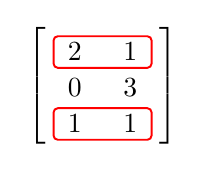
\begin{tikzpicture}[baseline=(m.center)]
\matrix (m) [matrix of math nodes, left delimiter={[}, right delimiter={]}, inner sep=1.5pt, column sep=5pt, row sep=2pt, nodes={minimum width=1.5em, minimum height=1.1em}] {2 & 1 \\ 0 & 3 \\ 1 & 1 \\};
\node[draw=red, line width=0.7pt, rounded corners=1.5pt, inner sep=0pt, fit=(m-1-1)(m-1-2)] {};
\node[draw=red, line width=0.7pt, rounded corners=1.5pt, inner sep=0pt, fit=(m-3-1)(m-3-2)] {};
\end{tikzpicture}
\quad\longmapsto\quad
\Wwrite^{\ell}G =
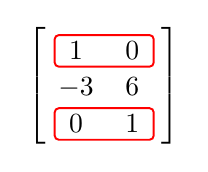
\begin{tikzpicture}[baseline=(m.center)]
\matrix (m) [matrix of math nodes, left delimiter={[}, right delimiter={]}, inner sep=1.5pt, column sep=5pt, row sep=2pt, nodes={minimum width=1.5em, minimum height=1.1em}] {1 & 0 \\ -3 & 6 \\ 0 & 1 \\};
\node[draw=red, line width=0.7pt, rounded corners=1.5pt, inner sep=0pt, fit=(m-1-1)(m-1-2)] {};
\node[draw=red, line width=0.7pt, rounded corners=1.5pt, inner sep=0pt, fit=(m-3-1)(m-3-2)] {};
\end{tikzpicture}
, \qquad G = W_1^{-1} = \begin{bmatrix} 1 & -1 \\ -1 & 2 \end{bmatrix},
\]
and the next read $\Wread^{\ell+1}$ to $G^{-1}\Wread^{\ell+1} = W_1\Wread^{\ell+1}$. The two outlined rows now hold $\dm^2 = 4$ fixed entries, and the other row has changed. Permuting the hidden units of the block moves the chosen rows next to each other. At generic parameters any $\dm$ rows form an invertible matrix, so in practice one takes a $\dm\times\dm$ block of the matrix, for example its first $\dm$ rows.
\end{example}

\subsection{LayerNorm, and the count for a ViT-B}\label{app:ln}

The reduction of LayerNorm to RMSNorm is standard: the centering folds into the adjacent weights \citep{elhage2021circuits}, and centering every write gives an RMSNorm network whose hidden states have mean zero \citep{ashkboos2024slicegpt,theus2025glmc}. We state it with the constants that the counts need.

\begin{proposition}[LayerNorm reduces to RMSNorm]\label{prop:ln}
Let $\mathbf 1$ be the column of $\dm$ ones, $Z = I - \tfrac1\dm\mathbf 1\mathbf 1^\top$, and $\mathcal V$ the space of the rows $h$ with $h\mathbf 1 = 0$. Consider a pre-LayerNorm network, whose reads and readout see $\mathrm{LN}(h) = \gamma\odot N_\varepsilon(hZ) + \beta$, with rows $\gamma$ and $\beta$ and the entrywise product $\odot$.\\
\stpart{prop:ln}{i}{} Replacing each read $W$ by $\mathrm{diag}(\gamma)W$ with the added bias $\beta W$, and each write $W$, write bias $b$ and embedding $E$ by $WZ$, $bZ$ and $EZ$, gives a network that computes the same function, whose hidden states lie in $\mathcal V$, and whose reads see $N_\varepsilon(h)$.\\
\stpart{prop:ln}{ii}{} In an orthonormal basis of $\mathcal V$, this network is a pre-RMSNorm network of dimension $\dm-1$, with every read multiplied by $\sqrt{\dm/(\dm-1)}$ and $\varepsilon$ replaced by $\varepsilon \dm/(\dm-1)$.
\end{proposition}

\begin{proof}
(i) A read satisfies $\mathrm{LN}(h)\,W = N_\varepsilon(hZ)\,\mathrm{diag}(\gamma)W + \beta W$. Every hidden state is the output of a write, so replacing every write, write bias and the embedding by its image under $Z$ replaces every hidden state $h$ by $hZ$. Since $Z^2 = Z$, every read then sees the same $N_\varepsilon(hZ)$ as before, and the function is unchanged; the hidden states lie in $\mathcal V$.
(ii) Let the columns of $\bar U \in \R^{\dm\times(\dm-1)}$ be an orthonormal basis of $\mathcal V$, written as columns, and $h = y\bar U^\top$ with a row $y$. Then
\[
\frac{\norm{h}^2}{\dm} + \varepsilon \;=\; \frac{\dm-1}{\dm}\Big(\frac{\norm{y}^2}{\dm-1} + \frac{\varepsilon\,\dm}{\dm-1}\Big),
\]
and therefore
\[
N_\varepsilon(y\bar U^\top) \;=\; \sqrt{\frac{\dm}{\dm-1}}\;N'(y)\,\bar U^\top ,
\]
where $N'$ is RMSNorm of dimension $\dm-1$ with the constant $\varepsilon \dm/(\dm-1)$. So a read $W$ of $N_\varepsilon(y\bar U^\top)$ is the read $\sqrt{\dm/(\dm-1)}\,\bar U^\top W$ of $N'(y)$, and a write $WZ$ is the write $W\bar U$ in the coordinates $y$.
\end{proof}

\para{The ViT-B of Ji et al.}\label{app:scale} The ViT-B that \citet{ji2026cutting} train without skip connections has $\dm = 768$ and $12$ layers, so $L = 24$ blocks and $25$ hidden states: one before each block and one before the readout. We assume standard pre-LayerNorm blocks, which reduce to RMSNorm of dimension $767$ by \cref{prop:ln}. By \cpref{prop:skipless}{ii}, one triangular $767\times767$ submatrix of a read per hidden state removes
\[
25\cdot\frac{767\cdot766}{2} \;=\; 7{,}344{,}025
\]
parameters, $8.5$ percent of the $86.6$M parameters of the model.

\section{Symmetries inside the blocks, and the upper bound}\label{app:prf-count}

\para{The symmetries inside the blocks, with their sources.} Permutations of hidden units or heads and sign flips of $\tanh$ hidden units are finite and remove no parameters \citep{hechtnielsen1989theory,sussmann1992,fefferman1994}. The continuous symmetries inside a block are the following, where $c_i$ is the read column of hidden unit $i$, or its gate column in a gated block, $e_i$ its value column, and $a_i$ its write row:
\begin{align*}
&\text{ReLU:} && (c_i, a_i) \mapsto (\lambda c_i,\ a_i/\lambda), && \lambda > 0;\\
&\text{ReLU}^2\text{:} && (c_i, a_i) \mapsto (\lambda c_i,\ a_i/\lambda^2), && \lambda > 0;\\
&\text{SwiGLU, GeGLU, ReGLU:} && (e_i, a_i) \mapsto (e_i/\lambda,\ \lambda a_i), && \lambda \neq 0;\\
&\text{ReGLU, in addition:} && (c_i, a_i) \mapsto (\lambda c_i,\ a_i/\lambda), && \lambda > 0;\\
&\text{attention, head } i\text{:} && (W_{Q,i}, W_{K,i}) \mapsto (W_{Q,i}K,\ W_{K,i}K^{-\top}), && K \in \GL(d_h);\\
& && (W_{V,i}, W_{O,i}) \mapsto (W_{V,i}K',\ K'^{-1}W_{O,i}), && K' \in \GL(d_h).
\end{align*}
Here $W_{Q,i}, W_{K,i}, W_{V,i} \in \R^{\dm\times d_h}$ and $W_{O,i} \in \R^{d_h\times\dm}$ are the matrices of head $i$. The rescaling of a ReLU hidden unit is well known \citep{rolnick2020reverse,petzka2020symmetries,godfrey2022symmetries}, and the changes of basis inside a head are those of \citet{elhage2021circuits} and \citet{theus2025glmc}. So a block has $s = \dhid$ for ReLU, ReLU$^2$, SwiGLU and GeGLU, $s = 2\dhid$ for ReGLU, $s = 2Hd_h^2$ for attention, and $s = 0$ for $\tanh$ and GELU. For a coordinate-wise activation $\sigma$, \citet[Theorem~E.14]{godfrey2022symmetries} determine the matrices $A$ with $\sigma\circ A = B\circ\sigma$ for some matrix $B$, and for GELU they are the permutation matrices (their Appendix~E.2.1).

The changes of basis of \cref{prop:cob} and the symmetries inside the blocks act \emph{locally freely} at $\theta$ if no continuous family of them, other than the identity, fixes $\theta$.

\begin{lemma}[Locally free action]\label{lem:free}
Without normalization or under pre-RMSNorm, consider a network whose blocks are $\tanh$, GELU, ReLU, ReLU$^2$ or gated blocks with at least $\dm$ hidden units, or attention blocks whose heads have width $d_h \le \dm$ and total width $Hd_h \ge \dm$. If $d_{\mathrm{in}} \ge \dm$, then at generic parameters the changes of basis and the symmetries inside the blocks act locally freely.
\end{lemma}

\begin{proof}
Let changes of basis $G_0, \dots, G_L \in \G$ and symmetries inside the blocks, all close to the identity, fix a generic $\theta$. The embedding becomes $EG_0 = E$, and $E$ has rank $\dm$, so $G_0 = I$. Suppose that $G_{\ell-1} = I$. In an MLP block, the read then becomes $\Wread^{\ell}\,\mathrm{diag}(\lambda)$, where $\lambda$ holds the numbers by which the symmetries inside the block multiply its columns, with entries $1$ on the columns that they leave alone. No column of a generic $\Wread^{\ell}$ vanishes, so every entry of $\lambda$ is $1$: for a ReGLU block this fixes both rescalings of every hidden unit, and for the other kinds the one rescaling. The write then becomes $\Wwrite^{\ell}G_\ell = \Wwrite^{\ell}$, and $\Wwrite^{\ell}$ has rank $\dm$ because the block has at least $\dm$ hidden units, so $G_\ell = I$. In an attention block, the changes of basis inside the heads map $W_{Q,i} \mapsto W_{Q,i}K_i$ and $W_{V,i} \mapsto W_{V,i}K'_i$. At generic parameters these matrices have full column rank, as $d_h \le \dm$, so $K_i = K'_i = I$. The write, which stacks the $W_{O,i}$, then becomes $W_OG_\ell = W_O$ and has rank $\dm$, as $Hd_h \ge \dm$, so $G_\ell = I$. By induction only the identity fixes $\theta$. For $\G = \Ort(\dm)$ the argument is the same.
\end{proof}

\begin{remark}[The width condition]\label{rem:attnfree}
The condition on the width is needed. At a hidden state that is written and read at rank $m < \dm$, the changes of basis that fix the parameters form a family of dimension $(\dm-m)^2$, so they move the parameters in only $2\dm m - m^2$ independent directions, as \citet[Proposition~C.3]{zhao2023symmetries} compute for one hidden layer.
\end{remark}

We recall \cref{thm:unlock}.
\thmUnlock*

\begin{proof}
If a continuous family of maps of the parameters preserves the function, then the function does not change to first order along any direction in which the family moves $\theta$. So these directions lie in the kernel of the Jacobian on every batch, and the functional dimension at $\theta$ is at most $P$ minus the dimension of their span. The changes of basis of \cref{prop:cob}, one copy of $\G$ per hidden state, and the symmetries inside the blocks commute with each other: the first multiply $\Wwrite^{\ell}$ on the right and $\Wread^{\ell+1}$ on the left, and the second multiply $\Wread^{\ell}$ on the right and $\Wwrite^{\ell}$ on the left. Together they form a group of dimension $(L+1)\dim\G + s$, which preserves the function and acts locally freely at generic parameters (\cref{lem:free}). So at generic parameters it moves $\theta$ in $(L+1)\dim\G + s$ independent directions.
\end{proof}

We recall \cref{prop:localid}.
\propLocalId*

\begin{proof}
Let $k = (L+1)\dim\G + s$ be the dimension of the symmetries of the network. Let $r$ be the largest rank that the Jacobian of $F_X$ attains on any batch $X$ at any parameters, and fix a batch $X$ that attains it. The outputs are analytic in $\theta$, so the rank on $X$ is $r$ outside the zero set of the sum of the squares of the minors of size $r$, a set of measure zero. Hence $r$ is the functional dimension at generic parameters, $r \le P - k$ by \cref{thm:unlock}, and the equality condition is $r = P - k$.

Take $\theta$ at which the rank on $X$ is $r$ and the symmetries act locally freely, as they do at generic parameters (\cref{lem:free}). By lower semicontinuity the rank on $X$ is $r$ on a neighborhood $U$ of $\theta$. By the constant rank theorem, after shrinking $U$, the set $\mathcal Z = \{\theta' \in U : F_X(\theta') = F_X(\theta)\}$ is a connected manifold of dimension $P - r$, whose tangent space at each point is the kernel of the Jacobian. For any further input $x$, the Jacobian on $X \cup \{x\}$ has rank $r$ on $U$ as well, so it has the same kernel, and $\theta' \mapsto F_{\theta'}(x)$ is constant on $\mathcal Z$. So $\mathcal Z = \{\theta' \in U : F_{\theta'} = F_\theta\}$. The changes of basis of \cref{prop:cob}, the rescalings and the changes of basis inside the heads form a Lie group of dimension $k$, which acts smoothly. It acts locally freely at $\theta$, so the map that sends an element of the group to the image of $\theta$ under it is an immersion near the identity, and it maps a neighborhood of the identity onto a manifold $\mathcal O \subset \mathcal Z$ of dimension $k$.

If $r = P - k$, then $\mathcal O$ is open in $\mathcal Z$, since the two have the same dimension. So every $\theta'$ close to $\theta$ with $F_{\theta'} = F_\theta$ is the image of $\theta$ under a symmetry close to the identity. Conversely, let every $\theta'$ in a neighborhood of $\theta$ in $\mathcal Z$ be the image of $\theta$ under a symmetry. With the permutations and the sign flips, the symmetries form a Lie group of dimension $k$ with finitely many components, and the images of $\theta$ under it form the image of a manifold of dimension $k$ under a smooth map. By Sard's theorem this image contains no open subset of a manifold of larger dimension, so $P - r \le k$, which with $r \le P - k$ is the equality condition.
\end{proof}

\section{The one-block theorem}\label{app:onelayer}

This appendix states and proves the general form of \cref{thm:oneblock}. With one block and without normalization, the network is $x \mapsto f(xE\Wread)\,\Wwrite D$.

\begin{theorem}[One block]\label{thm:onelayer}
Let $\dm \ge 2$ and $d_{\mathrm{in}}, d_{\mathrm{out}} \ge \dm$, let inputs range over all of $\R^{T\times d_{\mathrm{in}}}$, and consider networks with one block, without normalization and without biases. The block is a $\tanh$, GELU, ReLU, ReLU$^2$, ReGLU, SwiGLU or GeGLU block with at least $\dm$ hidden units, or an attention block of $H$ heads of width $d_h \le \dm$ with $Hd_h \ge \dm$, causal or not, on sequences of at least two tokens. At generic parameters the functional dimension is
\[
P - 2\dm^2 - s ,
\]
where $s$ is the dimension of the symmetries inside the block (\cref{app:prf-count}).
\end{theorem}

\para{Notation and flat directions.} We write $F(\theta, x)$ for the output of the network at the parameters $\theta \in \R^P$ and the input $x$, and $\Der_\theta F(\theta, x)$ for the Fr\'echet derivative of $F(\cdot, x)$ at $\theta$, a linear map on $\R^P$. The derivative is written with an upright $\Der$ so that it is not confused with the readout matrix $D$ of the network. For a direction $\eta \in \R^P$, $\Der_\theta F(\theta, x)\,\eta$ is the derivative of $\tau \mapsto F(\theta + \tau\eta, x)$ at $\tau = 0$. We write $\eta_E$, $\eta_D$, $\eta_{\mathrm{read}}$ and $\eta_{\mathrm{write}}$ for the entries of $\eta$ at the positions of $E$, $D$, $\Wread$ and $\Wwrite$, and $\Der_\theta Q\,\eta$ for the derivative along $\eta$ of a matrix $Q$ that depends on the parameters; for instance $\Der_\theta C\,\eta = \eta_E\Wread + E\,\eta_{\mathrm{read}}$ for $C = E\Wread$, by the product rule. Call $\eta$ \emph{flat} if $\Der_\theta F(\theta, x)\,\eta = 0$ for every input $x$, and let $\mathcal K(\theta)$ be the space of flat directions. For ReLU, ReLU$^2$ and ReGLU blocks, $F(\theta, x)$ is differentiable in $\theta$ at the inputs $x$ at which no hidden unit sits at its kink, which form an open set of full measure, and ``every input'' means every such input. For a batch of inputs $x_1, \dots, x_n$, the Jacobian of $\theta \mapsto (F(\theta, x_1), \dots, F(\theta, x_n))$ is the matrix of the linear map $\eta \mapsto (\Der_\theta F(\theta, x_1)\,\eta, \dots, \Der_\theta F(\theta, x_n)\,\eta)$. It has $P$ columns, and its kernel consists of the directions with $\Der_\theta F(\theta, x_k)\,\eta = 0$ for the inputs of the batch. Adding inputs can only shrink this kernel, and a decreasing chain of subspaces of $\R^P$ stops, so some finite batch has the kernel $\mathcal K(\theta)$. By rank--nullity, the functional dimension at $\theta$ is therefore
\[
P - \dim\mathcal K(\theta).
\]
The theorem thus amounts to finding the flat directions.

\para{Overview.} For an MLP block, the parameters enter the function only through $C = E\Wread$ and $A = \Wwrite D$. Step~1 finds the directions that keep these two matrices fixed: they are the directions in which the changes of basis at $h_0$ and at $h_1$ move the parameters. Step~2 shows that a flat direction changes $C$ and $A$ only along the symmetries of the hidden units: each hidden unit is isolated, by its kink for ReLU, ReLU$^2$ and ReGLU, and for $\tanh$, GELU, SwiGLU and GeGLU by how fast it approaches its limit on rays $x = tn$ with $t \to \infty$. Step~3 counts. For an attention block the same steps run with one factorization per head, and inputs of two tokens turn Step~2 into the case of $\tanh$.

\subsection*{MLP blocks}

\para{Reduction.} An MLP block acts on each token separately, so we take $T = 1$. The network computes $F(\theta, x) = f(xC)\,A$. For a $\tanh$, GELU, ReLU or ReLU$^2$ block let $c_i$ be the columns of $C$, one per hidden unit, $a_i$ the rows of $A$, and $z_i = xc_i$, so that $F(\theta, x) = \sum_i \sigma(z_i)\,a_i$. For a gated block, $C = [\,EW_g \mid EW_v\,]$, hidden unit $i$ has the gate column $c_i$, a column of $EW_g$, and the value column $e_i$, a column of $EW_v$, and $F(\theta, x) = \sum_i \sigma(xc_i)\,(xe_i)\,a_i$. For generic parameters $E$, $D$, $\Wread$ and $\Wwrite$ have rank $\dm$, every $a_i$ is nonzero, and the $c_i$ are nonzero and pairwise non-collinear: they lie in the column space of $E$, of dimension $\dm \ge 2$, where two generic vectors are not collinear. In a gated block, in the same way, every $e_i$ is nonzero and is not proportional to $c_i$.

\needspace{5\baselineskip}
\para{Step 1: changes of basis.} We need the following lemma.
\begin{nested}
\begin{lemma}[The directions that keep $C$ and $A$]\label{lem:fact}
Let $E$, $D$, $\Wread$ and $\Wwrite$ have rank $\dm$. A direction $\eta$ keeps $C$ and $A$ fixed to first order, $\Der_\theta C\,\eta = 0$ and $\Der_\theta A\,\eta = 0$, if and only if
\[
\eta_E = EX,\qquad \eta_{\mathrm{read}} = -X\Wread,\qquad \eta_{\mathrm{write}} = \Wwrite Y,\qquad \eta_D = -YD
\]
for some $X, Y \in \R^{\dm\times\dm}$. The matrices $X$ and $Y$ are determined by the direction, so these directions form a space of dimension $2\dm^2$.
\end{lemma}

\begin{proof}
Since $\Wread$ has rank $\dm$, it has a right inverse $R$, with $\Wread R = I$, and $E$, of rank $\dm$ with $\dm$ columns, has a left inverse. From $\Der_\theta C\,\eta = \eta_E\Wread + E\eta_{\mathrm{read}} = 0$, multiplying on the right by $R$ gives $\eta_E = EX$ with $X = -\eta_{\mathrm{read}}R$; then $E\eta_{\mathrm{read}} = -EX\Wread$, and cancelling $E$ on the left gives $\eta_{\mathrm{read}} = -X\Wread$. In the same way, $D$ has a right inverse and $\Wwrite$ a left inverse, and $\Der_\theta A\,\eta = \eta_{\mathrm{write}}D + \Wwrite\eta_D = 0$ gives $\eta_{\mathrm{write}} = \Wwrite Y$ and $\eta_D = -YD$. Conversely these directions give $\Der_\theta C\,\eta = EX\Wread - EX\Wread = 0$ and $\Der_\theta A\,\eta = 0$. Finally $\eta_E = EX$ determines $X$, and $\eta_D = -YD$ determines $Y$.
\end{proof}
\end{nested}

These are the directions in which the changes of basis $I + \tau X$ at $h_0$ and $I + \tau Y$ at $h_1$ move the parameters.

\para{Step 2: hidden units.} We need a lemma on the function
\[
G(\phi, x) = xM + \gamma + \textstyle\sum_i \sigma(z_i)\,a_i,\qquad z_i = xc_i + \beta_i,
\]
of the matrices $\phi = \big(M, \gamma, (c_i, \beta_i, a_i)_i\big)$ themselves. For a direction $\psi$ of $\phi$, with entries $\psi_M$, $\psi_\gamma$, $\psi_{c_i}$, $\psi_{\beta_i}$ and $\psi_{a_i}$, the Fr\'echet derivative of $G(\cdot, x)$ at $\phi$ gives
\begin{equation}\label{eq:dotF}
\Der_\phi G(\phi, x)\,\psi = x\psi_M + \psi_\gamma + \sum_i \big[\sigma(z_i)\,\psi_{a_i} + \sigma'(z_i)\,(x\psi_{c_i} + \psi_{\beta_i})\,a_i\big].
\end{equation}
A gated unit computes $\sigma(z_i)\,w_i\,a_i$ with a gate $z_i = xc_i + \beta_i$ and a value $w_i = xe_i + \beta'_i$, where $\sigma(z) = \max(z, 0)$ for ReGLU, $z/(1 + e^{-z})$ for SwiGLU and $z\Phi(z)$ for GeGLU, so that $\phi$ also contains the $e_i$ and $\beta'_i$, and the terms of the unit in $\Der_\phi G(\phi, x)\,\psi$ are $\sigma(z_i)\,w_i\,\psi_{a_i} + \sigma'(z_i)\,(x\psi_{c_i} + \psi_{\beta_i})\,w_i\,a_i + \sigma(z_i)\,(x\psi_{e_i} + \psi_{\beta'_i})\,a_i$.

\begin{nested}
\begin{lemma}[A flat direction only rescales units]\label{lem:unitid}
Let every $a_i \neq 0$ and let the $c_i$ be nonzero and pairwise non-collinear; for the gated blocks let also every $e_i \neq 0$, with $(e_i, \beta'_i)$ not proportional to $(c_i, \beta_i)$. If $\Der_\phi G(\phi, x)\,\psi = 0$ for all $x$, then $\psi_M = 0$, $\psi_\gamma = 0$, and for every unit $i$:\\
for $\tanh$ and GELU, $\psi_{a_i} = 0$, $\psi_{c_i} = 0$ and $\psi_{\beta_i} = 0$;\\
for ReLU, $(\psi_{c_i}, \psi_{\beta_i}) = \lambda_i(c_i, \beta_i)$ and $\psi_{a_i} = -\lambda_ia_i$ for some number $\lambda_i$;\\
for ReLU$^2$, $(\psi_{c_i}, \psi_{\beta_i}) = \lambda_i(c_i, \beta_i)$ and $\psi_{a_i} = -2\lambda_ia_i$;\\
for ReGLU, $(\psi_{c_i}, \psi_{\beta_i}) = \lambda_i(c_i, \beta_i)$, $(\psi_{e_i}, \psi_{\beta'_i}) = -\alpha_i(e_i, \beta'_i)$ and $\psi_{a_i} = (\alpha_i - \lambda_i)a_i$ for some numbers $\lambda_i$ and $\alpha_i$;\\
for SwiGLU and GeGLU, $\psi_{c_i} = 0$, $\psi_{\beta_i} = 0$, $(\psi_{e_i}, \psi_{\beta'_i}) = -\alpha_i(e_i, \beta'_i)$ and $\psi_{a_i} = \alpha_ia_i$ for some number $\alpha_i$.
\end{lemma}

\begin{proof}
Let $H_i = \{x : z_i = 0\}$, a hyperplane since $c_i \neq 0$. Since the $c_i$ are pairwise non-collinear, the $H_i$ are pairwise non-parallel, so every $H_i$ contains points that lie on no other $H_k$. We use one fact from linear algebra: an affine function that vanishes on an open piece of $H_i$ is a multiple of $z_i$, since it vanishes on all of $H_i$ and $H_i$ has codimension one. We write $J(x) = \Der_\phi G(\phi, x)\,\psi$, a function of $x$ alone, which vanishes by assumption.

\emph{ReLU.} Here $\sigma' = \mathbf 1[z > 0]$ jumps at $0$. Near a point $x_0$ of $H_i$ that lies on no other $H_k$, every term of \cref{eq:dotF} is continuous except $\mathbf 1[z_i > 0](x\psi_{c_i} + \psi_{\beta_i})\,a_i$, which jumps by $(x_0\psi_{c_i} + \psi_{\beta_i})\,a_i$ as $x$ crosses $H_i$ at $x_0$. As $J = 0$ is continuous, this jump vanishes, and since $a_i \neq 0$, the affine function $x\psi_{c_i} + \psi_{\beta_i}$ vanishes on an open piece of $H_i$, so $(\psi_{c_i}, \psi_{\beta_i}) = \lambda_i(c_i, \beta_i)$. The terms of unit $i$ then add up to $\max(z_i, 0)\,(\psi_{a_i} + \lambda_ia_i)$, since $z\,\mathbf 1[z > 0] = \max(z, 0)$. Across $H_i$, the gradient of $J$ with respect to $x$ jumps by the matrix $c_i(\psi_{a_i} + \lambda_ia_i)$, which must vanish, so $\psi_{a_i} = -\lambda_ia_i$. With every unit removed in this way, $J(x) = x\psi_M + \psi_\gamma = 0$ for all $x$ gives $\psi_M = 0$ and $\psi_\gamma = 0$.

\emph{ReLU$^2$.} The same argument one derivative higher: $\sigma'(z) = 2\max(z, 0)$ is continuous, and across $H_i$ the gradient of $2\max(z_i, 0)(x\psi_{c_i} + \psi_{\beta_i})\,a_i$ jumps by $2c_i(x_0\psi_{c_i} + \psi_{\beta_i})\,a_i$, which forces $(\psi_{c_i}, \psi_{\beta_i}) = \lambda_i(c_i, \beta_i)$. The terms of unit $i$ then add up to $\max(z_i, 0)^2(\psi_{a_i} + 2\lambda_ia_i)$, whose second derivative jumps across $H_i$, so $\psi_{a_i} = -2\lambda_ia_i$.

\emph{ReGLU.} As $(e_i, \beta'_i)$ is nonzero and not proportional to $(c_i, \beta_i)$, the affine function $w_i$ does not vanish on all of $H_i$, so it is nonzero on an open piece of $H_i$ that meets no other $H_k$; we take $x_0$ there. Across $H_i$ the terms of unit $i$ jump by $(x_0\psi_{c_i} + \psi_{\beta_i})\,w_i(x_0)\,a_i$, so $(\psi_{c_i}, \psi_{\beta_i}) = \lambda_i(c_i, \beta_i)$ as before. The terms of unit $i$ then add up to $\max(z_i, 0)\,V_i(x)$ with the affine function $V_i(x) = w_i(x)\,(\psi_{a_i} + \lambda_ia_i) + (x\psi_{e_i} + \psi_{\beta'_i})\,a_i$. The jump of their gradient across $H_i$ is $c_iV_i(x_0)$, so $V_i$ vanishes on an open piece of $H_i$, and $V_i(x) = z_i\,\nu_i$ for a row vector $\nu_i$. The terms of unit $i$ then add up to $\max(z_i, 0)^2\,\nu_i$, whose second derivative jumps across $H_i$, so $\nu_i = 0$ and $V_i = 0$ for all $x$: $w_i(x)\,(\psi_{a_i} + \lambda_ia_i) = -(x\psi_{e_i} + \psi_{\beta'_i})\,a_i$. Both sides are products of an affine function of $x$ and a fixed row vector, and $a_i \neq 0$, so $\psi_{a_i} + \lambda_ia_i = \alpha_ia_i$ and $(\psi_{e_i}, \psi_{\beta'_i}) = -\alpha_i(e_i, \beta'_i)$ for some number $\alpha_i$. Then $\psi_M = 0$ and $\psi_\gamma = 0$ as for ReLU.

\emph{$\tanh$.} We restrict \cref{eq:dotF} to a ray $x = tn$, $t > 0$, with a direction $n$ such that the numbers $u_k = nc_k$ are all nonzero and $\lvert u_j\rvert < \lvert u_k\rvert$ for one unit $j$ and all $k \neq j$. For each $j$ and each sign $s = \pm 1$, the directions $n$ with $su_j > 0$ and this property form a nonempty open set: start from a point of the hyperplane $nc_j = 0$ where no other $nc_k$ vanishes, and move a little to the side $s$. For $z > 0$,
\begin{gather*}
\tanh z = 1 - 2e^{-2z} + r(z),\quad 0 \le r(z) \le 2e^{-4z},\\
\tanh' z = 4e^{-2z} - q(z),\quad 0 \le q(z) \le 8e^{-4z},
\end{gather*}
from $\tanh z = (1 - e^{-2z})/(1 + e^{-2z})$ and $\tanh' = 1 - \tanh^2$, and $\tanh$ is odd. On the ray $z_k = u_kt + \beta_k$, so for large $t$ the terms of unit $k$ in \cref{eq:dotF} are
\[
s_k\psi_{a_k} + e^{-2\lvert u_k\rvert t}\,e^{-2s_k\beta_k}\big[-2s_k\psi_{a_k} + 4\,(t\,n\psi_{c_k} + \psi_{\beta_k})\,a_k\big] + O\big((1+t)\,e^{-4\lvert u_k\rvert t}\big),
\]
with $s_k$ the sign of $u_k$. All terms of $J(tn)$ are therefore $t\,n\psi_M$, a constant, the bracket of unit $j$ times $e^{-2\lvert u_j\rvert t}$, and terms that are $O\big((1+t)e^{-\rho t}\big)$ with $\rho = \min\big(4\lvert u_j\rvert, \min_{k\neq j}2\lvert u_k\rvert\big) > 2\lvert u_j\rvert$. As $J(tn) = 0$ for all $t$, dividing by $t$ and letting $t \to \infty$ gives $n\psi_M = 0$; then the constant vanishes; then multiplying by $e^{2\lvert u_j\rvert t}$ and letting $t \to \infty$ shows that the bracket of unit $j$, a polynomial of degree one in $t$, tends to zero, so both of its coefficients vanish: $(n\psi_{c_j})\,a_j = 0$ and $2\psi_{\beta_j}a_j = s\,\psi_{a_j}$. As $a_j \neq 0$, $n\psi_{c_j} = 0$ for all $n$ in an open set, so $\psi_{c_j} = 0$; and the two signs $s = \pm1$ give $\psi_{a_j} = 2\psi_{\beta_j}a_j = -2\psi_{\beta_j}a_j$, so $\psi_{\beta_j} = 0$ and $\psi_{a_j} = 0$. This holds for every unit $j$, and then $J(x) = x\psi_M + \psi_\gamma = 0$ gives $\psi_M = 0$ and $\psi_\gamma = 0$.

\emph{GELU.} Here $\sigma(z) = z\Phi(z)$, with $\Phi$ the standard normal distribution function and $\varphi = \Phi'$ its density. The tail $\bar\Phi = 1 - \Phi$ satisfies $\varphi(z)(1/z - 1/z^3) \le \bar\Phi(z) \le \varphi(z)/z$ for $z > 0$, as one checks by differentiating, and $\Phi(-z) = 1 - \Phi(z)$ carries these bounds to $z < 0$. From these, as $\lvert z\rvert \to \infty$ on either side,
\begin{gather*}
\sigma(z) = \max(z, 0) - \varphi(z) + O\big(\varphi(z)/z^2\big),\\
\sigma'(z) = \mathbf 1[z > 0] + \varphi(z)\,(z - 1/z) + O\big(\varphi(z)/\lvert z\rvert^3\big).
\end{gather*}
Take a ray $x = tn$ as for $\tanh$. The terms of unit $k$ in \cref{eq:dotF} split into a polynomial of degree at most one in $t$, from $\max(z, 0)$ and $\mathbf 1[z > 0]$, and the Gaussian part
\begin{multline*}
\varphi(z_k)\,\Big[u_k\,(n\psi_{c_k})\,t^2 + \big(u_k\psi_{\beta_k} + \beta_k\,n\psi_{c_k}\big)\,t + \beta_k\psi_{\beta_k} - (n\psi_{c_k})/u_k\Big]a_k\\
-\; \varphi(z_k)\,\psi_{a_k} \;+\; O\big(\varphi(z_k)/t\big).
\end{multline*}
Gaussian parts tend to zero faster than any power of $t$, so as $J(tn) = 0$ for all $t$, the polynomial part vanishes, and so does the sum of the Gaussian parts. For $k \neq j$, $\varphi(z_k)/\varphi(z_j) = \exp\big(-\tfrac12(u_k^2 - u_j^2)\,t^2 + O(t)\big)$ tends to zero faster than any power of $t$, since $u_k^2 > u_j^2$. Dividing the sum of the Gaussian parts by $\varphi(z_j)$ and letting $t \to \infty$ therefore makes the coefficients of $t^2$, $t$ and $1$ in the bracket of unit $j$ vanish, in this order: $u_j(n\psi_{c_j})\,a_j = 0$, so $n\psi_{c_j} = 0$; then $u_j\psi_{\beta_j}\,a_j = 0$, so $\psi_{\beta_j} = 0$; then $\psi_{a_j} = 0$. As for $\tanh$, $n\psi_{c_j} = 0$ on an open set gives $\psi_{c_j} = 0$, and finally $\psi_M = 0$ and $\psi_\gamma = 0$.

\emph{SwiGLU and GeGLU.} Take a ray $x = tn$ as for $\tanh$, and write $v_k = ne_k$, so that $w_k = v_kt + \beta'_k$; as $e_j \neq 0$, also $v_j \neq 0$ on an open set of such $n$. For SwiGLU, $\sigma(z) = z - z/(1 + e^z)$ gives, as $\lvert z\rvert \to \infty$ with $s$ the sign of $z$,
\begin{gather*}
\sigma(z) = \max(z, 0) - \lvert z\rvert e^{-\lvert z\rvert} + O\big(\lvert z\rvert e^{-2\lvert z\rvert}\big),\\
\sigma'(z) = \mathbf 1[z > 0] + s\,(\lvert z\rvert - 1)\,e^{-\lvert z\rvert} + O\big(\lvert z\rvert e^{-2\lvert z\rvert}\big).
\end{gather*}
The terms of unit $k$ in \cref{eq:dotF} then split into a polynomial in $t$, from $\max(z, 0)$ and $\mathbf 1[z > 0]$, and a rest that is $e^{-\lvert z_k\rvert}$ times a polynomial in $t$, up to $O(t^3e^{-2\lvert z_k\rvert})$; for GeGLU, with the expansions of GELU, the rest is $\varphi(z_k)$ times a polynomial in $t$ and $1/z_k$, up to $O(\varphi(z_k)/t)$. As for $\tanh$ and GELU, the polynomial parts vanish, and dividing the sum of the rests by $e^{-\lvert z_j\rvert}$, respectively $\varphi(z_j)$, and letting $t \to \infty$ shows that the rest of the slowest unit $j$ vanishes. For SwiGLU this rest is $e^{-\lvert z_j\rvert}$ times
\[
s\,(\lvert z_j\rvert - 1)\,(t\,n\psi_{c_j} + \psi_{\beta_j})\,w_j\,a_j - \lvert z_j\rvert\big((t\,n\psi_{e_j} + \psi_{\beta'_j})\,a_j + w_j\,\psi_{a_j}\big),
\]
with $s$ the sign of $u_j$ and $\lvert z_j\rvert = \lvert u_j\rvert t + s\beta_j$, a polynomial of degree three in $t$, whose coefficients therefore vanish. The coefficient of $t^3$ is $s\lvert u_j\rvert\,(n\psi_{c_j})\,v_j\,a_j$, so $\psi_{c_j} = 0$ as for $\tanh$. The coefficient of $t^2$ is then $-\lvert u_j\rvert\big((n\psi_{e_j})\,a_j + v_j(\psi_{a_j} - s\psi_{\beta_j}a_j)\big)$. As it vanishes for all $n$ in an open set, $\psi_{e_j} = -\alpha e_j$ and $\psi_{a_j} - s\psi_{\beta_j}a_j = \alpha a_j$ for a number $\alpha$, the same for both signs since $\psi_{e_j}$ is; the two signs then give $\psi_{\beta_j} = 0$. The coefficient of $t$ is then $-\lvert u_j\rvert(\psi_{\beta'_j} + \alpha\beta'_j)\,a_j$, so $\psi_{\beta'_j} = -\alpha\beta'_j$. For GeGLU the rest of unit $j$ is $\varphi(z_j)$ times the same bracket with $z_j - 1/z_j$ in place of $s(\lvert z_j\rvert - 1)$ and $1$ in place of $\lvert z_j\rvert$, and its coefficients of $t^3$, $t^2$, $t$ and $1$ give, in this order, $\psi_{c_j} = 0$, $\psi_{\beta_j} = 0$, $(\psi_{e_j}, \psi_{a_j}) = (-\alpha e_j, \alpha a_j)$ and $\psi_{\beta'_j} = -\alpha\beta'_j$. In both cases the terms of unit $j$ then vanish; this holds for every unit, and $\psi_M = 0$ and $\psi_\gamma = 0$ as for $\tanh$.
\end{proof}
\end{nested}

The lemma is stated with a linear term $xM$, a constant $\gamma$ and biases $\beta_i$ and $\beta'_i$, which cost nothing in its proof. For the MLP blocks of this paper they all vanish, and the attention blocks below use them. For $\tanh$, the proof on rays follows that of Lemma~3.1 of \citet{sussmann1992}. For ReLU, the proof at the hyperplanes $H_i$ follows those of \citet[Lemma~2]{petzka2020symmetries} and \citet[Theorem~6]{stock2021embedding}. The directions left by the lemma are those of the rescalings of the hidden units (\cref{app:prf-count}).

\para{Step 3: counting.} Let $\eta$ be flat. The network depends on $\theta$ only through the columns and rows $c_i$, $e_i$ and $a_i$ of $C$ and $A$, and $F(\theta, x)$ is the function $G(\phi, x)$ of \cref{lem:unitid} with $M = 0$, $\gamma = 0$ and all biases zero. By the chain rule, the direction $\psi$ that holds the derivatives of the $c_i$, $e_i$ and $a_i$ along $\eta$, and zeros at $M$, $\gamma$ and the biases, satisfies $\Der_\phi G(\phi, x)\,\psi = \Der_\theta F(\theta, x)\,\eta = 0$ for all $x$. By \cref{lem:unitid} there are numbers $\lambda_i$ and $\alpha_i$ such that
\[
\Der_\theta C\,\eta \;=\; \big[\,EW_g\,\mathrm{diag}(\lambda) \;\big|\; -EW_v\,\mathrm{diag}(\alpha)\,\big], \qquad \Der_\theta A\,\eta \;=\; \mathrm{diag}(\mu)\,A
\]
for a gated block, with $\mu_i = \alpha_i - \lambda_i$, and with $\lambda = 0$ for SwiGLU and GeGLU; and $\Der_\theta C\,\eta = C\,\mathrm{diag}(\lambda)$, $\Der_\theta A\,\eta = \mathrm{diag}(\mu)\,A$ for the other blocks, with $\mu_i = -\lambda_i$ for ReLU, $\mu_i = -2\lambda_i$ for ReLU$^2$, and $\lambda = 0$, $\mu = 0$ for $\tanh$ and GELU. The direction $\eta^{\mathrm{sc}}$ with the entries
\begin{gather*}
\eta^{\mathrm{sc}}_{\mathrm{read}} = \big[\,W_g\,\mathrm{diag}(\lambda) \;\big|\; -W_v\,\mathrm{diag}(\alpha)\,\big] \ \text{ for a gated block}, \\
\eta^{\mathrm{sc}}_{\mathrm{read}} = \Wread\,\mathrm{diag}(\lambda) \ \text{ for the other blocks},\\
\eta^{\mathrm{sc}}_{\mathrm{write}} = \mathrm{diag}(\mu)\,\Wwrite, \qquad \eta^{\mathrm{sc}}_E = 0, \qquad \eta^{\mathrm{sc}}_D = 0
\end{gather*}
is the direction of a rescaling of the hidden units, and along it $C$ and $A$ have the same derivatives as along $\eta$. So $\eta - \eta^{\mathrm{sc}}$ keeps $C$ and $A$ fixed to first order, and \cref{lem:fact} describes it. Hence every flat direction is the sum of a direction of the changes of basis of \cref{lem:fact} and of a rescaling of the hidden units, and conversely all of these are flat, since they come from symmetries. The two kinds are independent: a rescaling that is also a direction of \cref{lem:fact} has $EX = 0$, so $X = 0$, and then its entry at the read vanishes, so every $\lambda_i$ and $\alpha_i$ is zero, because no column of $\Wread$ vanishes. So
\[
\dim\mathcal K(\theta) \;=\; 2\dm^2 + s ,
\]
where $s$ is the number of the rescalings: $\dhid$ for ReLU, ReLU$^2$, SwiGLU and GeGLU, $2\dhid$ for ReGLU, and none for $\tanh$ and GELU. The functional dimension $P - \dim\mathcal K(\theta)$ is the value of the theorem.

\subsection*{Attention blocks}

\para{Reduction.} Let $W_{Q,i}, W_{K,i}, W_{V,i} \in \R^{\dm\times d_h}$ and $W_{O,i} \in \R^{d_h\times\dm}$ be the matrices of head $i$, and let
\[
B_i = EW_{Q,i}W_{K,i}^\top E^\top/\sqrt{d_h}, \qquad C_i = EW_{V,i}W_{O,i}D, \qquad S = \textstyle\sum_i C_i .
\]
Let $x_t$ be row $t$ of the input $x$. Head $i$ gives token $t$ the scores $x_tB_ix_s^\top$ and the weights $a^{(i)}_{ts}$, their softmax over the tokens $s$ that token $t$ sees, and the output at token $t$ is $\sum_i\sum_s a^{(i)}_{ts}\,x_sC_i$. So the parameters enter only through these matrices. We use inputs of two kinds: with a causal mask, any sequence, whose second token sees only the first two; without a mask, sequences whose tokens other than the second all equal the first. Let $k$ be the number of tokens other than the second that the second token sees, $k = 1$ with a mask and $k = T - 1$ without. With $u = x_2$ and $v = x_2 - x_1$, head $i$ puts the weight $1/(1 + k\,e^{-uB_iv^\top})$ on the second token and the rest on the copies of the first, and $1/(1 + e^{-z}) = \tfrac12 + \tfrac12\tanh(z/2)$ gives the output at the second token
\begin{equation}\label{eq:twotok}
y_2 = uS - \tfrac12\,vS + \tfrac12\sum_i \tanh\big(\tfrac12(uB_iv^\top - \log k)\big)\,vC_i .
\end{equation}

\para{Step 1: the directions that keep $B_i$ and $C_i$.} For generic parameters $E$ and $D$ have rank $\dm$; every $W_{Q,i}$, $W_{K,i}$, $W_{V,i}$ and $W_{O,i}^\top$ has rank $d_h$, since $d_h \le \dm$; and the queries $[W_{Q,1}, \dots, W_{Q,H}] \in \R^{\dm\times Hd_h}$, the keys $[W_{K,1}, \dots, W_{K,H}]$ and the output projection $W_O \in \R^{Hd_h\times\dm}$ of all heads have rank $\dm$, since $Hd_h \ge \dm$. Write $\eta_{Q,i}$, $\eta_{K,i}$, $\eta_{V,i}$ and $\eta_{O,i}$ for the entries of a direction $\eta$ at the positions of $W_{Q,i}$, $W_{K,i}$, $W_{V,i}$ and $W_{O,i}$, and consider a direction with $\Der_\theta B_i\,\eta = 0$ and $\Der_\theta C_i\,\eta = 0$ for every head. Multiplying $\Der_\theta B_i\,\eta = 0$ on the left by the projection $I - EE^+$ onto the orthogonal complement of the column space of $E$, where $E^+$ is the pseudo-inverse, leaves $(I - EE^+)\,\eta_E\,W_{Q,i}W_{K,i}^\top E^\top = 0$. As $W_{K,i}^\top E^\top$ has full row rank, $(I - EE^+)\,\eta_E\,W_{Q,i} = 0$ for every head, and as the queries of all heads have rank $\dm$, $\eta_E = EX$ with $X = E^+\eta_E$. In the same way, multiplying $\Der_\theta C_i\,\eta = 0$ on the right by the projection $I - D^+D$ gives $\eta_D = -YD$ with $Y = -\eta_D\,D^+$, because $EW_{V,i}$ has full column rank and the output projection has rank $\dm$. Substituting, and cancelling $E$ on the left and $E^\top$ or $D$ on the right,
\begin{gather*}
(\eta_{Q,i} + XW_{Q,i})W_{K,i}^\top + W_{Q,i}(\eta_{K,i} + XW_{K,i})^\top = 0,\\
(\eta_{V,i} + XW_{V,i})W_{O,i} + W_{V,i}(\eta_{O,i} - W_{O,i}Y) = 0.
\end{gather*}
If $P_1$ and $P_2$ have full column rank and $Z_1P_2^\top + P_1Z_2^\top = 0$, then multiplying on the right by a right inverse of $P_2^\top$ gives $Z_1 = P_1\Gamma$ for a square matrix $\Gamma$, and then $Z_2 = -P_2\Gamma^\top$. Hence
\begin{gather*}
\eta_{Q,i} = -XW_{Q,i} + W_{Q,i}\Gamma_i, \qquad \eta_{K,i} = -XW_{K,i} - W_{K,i}\Gamma_i^\top, \\
\eta_{V,i} = -XW_{V,i} + W_{V,i}\Gamma'_i, \qquad \eta_{O,i} = W_{O,i}Y - \Gamma'_iW_{O,i} .
\end{gather*}
These are the directions of the changes of basis $I + \tau X$ at $h_0$ and $I + \tau Y$ at $h_1$, and of $I + \tau \Gamma_i$ between the queries and keys and $I + \tau \Gamma'_i$ between the values and outputs of head $i$. They are independent: $EX = 0$ forces $X = 0$, $YD = 0$ forces $Y = 0$, and then $W_{Q,i}\Gamma_i = 0$ and $W_{V,i}\Gamma'_i = 0$ force $\Gamma_i = \Gamma'_i = 0$.

\para{Step 2: two tokens.} For generic parameters and generic $v$ the columns $B_iv^\top$ are nonzero and pairwise non-collinear, since $\dm \ge 2$, and every row $vC_i$ is nonzero. For such a $v$, \eqref{eq:twotok} is, as a function of $u$, the function $G$ of \cref{lem:unitid} with one $\tanh$ hidden unit per head: unit $i$ has the read column $\tfrac12B_iv^\top$, the bias $-\tfrac12\log k$ and the write row $\tfrac12vC_i$, the linear term is $uS$, and the constant is $-\tfrac12vS$. Along a flat direction $\eta$ these have the derivatives $\tfrac12(\Der_\theta B_i\,\eta)v^\top$, $0$, $\tfrac12v(\Der_\theta C_i\,\eta)$, $\Der_\theta S\,\eta$ and $-\tfrac12v(\Der_\theta S\,\eta)$, and \cref{lem:unitid} for $\tanh$ shows that all of these vanish. This holds for all $v$ in an open set, so $\Der_\theta B_i\,\eta = 0$ and $\Der_\theta C_i\,\eta = 0$ for every head.

\para{Step 3: counting.} Every direction of Step~1 is flat, since it comes from a symmetry, and by Step~2 every flat direction, already on the inputs of \eqref{eq:twotok}, is one of them. So $\dim\mathcal K(\theta) = 2\dm^2 + 2Hd_h^2$, and $s = 2Hd_h^2$ for an attention block.

\begin{proof}[Proof of \cref{thm:oneblock}]
Within the scope of \cref{sec:setup}, it is \cref{thm:onelayer}: the functional dimension is the bound of \cref{thm:unlock} for $L = 1$ without normalization.
\end{proof}

\begin{remark}[One $\tanh$ block, from the theorem of Sussmann]\label{rem:sussmann}
For a $\tanh$ block, \cref{thm:oneblock} also follows from Theorem~2.1 of \citet{sussmann1992}. That theorem concerns networks with one hidden layer of $\tanh$ hidden units and one output,
\[
x \;\mapsto\; \tanh\Big(\gamma + \sum_{j}\alpha_j\,\tanh(xc_j + \beta_j)\Big),
\]
with numbers $\alpha_j$, $\beta_j$ and $\gamma$. It calls such a network irreducible if no $\alpha_j$ and no $c_j$ vanishes and $(c_i, \beta_i) \neq \pm(c_j, \beta_j)$ for $i \neq j$. It says that two irreducible networks with the same function have the same number of hidden units, and differ by a permutation of the hidden units and by sign flips $(c_j, \beta_j, \alpha_j) \mapsto (-c_j, -\beta_j, -\alpha_j)$. \citet{albertini1993uniqueness} give another proof of that theorem and extend it to other odd activations. For networks without biases, as here, their Lemmas~2.2 and~2.4 give it for every odd real-analytic activation that is not a polynomial. With several outputs and without biases, the statement is contained in Proposition~4.1 of \citet{albertini1993discrete}, the first step of their theorem on recurrent networks in discrete time.

The outer $\tanh$ is injective. So each of the $d_{\mathrm{out}}$ outputs of the network $x \mapsto \sum_i \tanh(xc_i)\,a_i$ of this appendix is the function of such a network, with $\beta_i = 0$, $\gamma = 0$ and with $\alpha_i$ an entry of $a_i$. At generic parameters these networks are irreducible, and so are those of all nearby parameters. So nearby parameters with the same function have the same columns $c_i$ and rows $a_i$, up to a permutation and sign flips of the hidden units, which are the identity for parameters that are close enough. They then have the same $C = E\Wread$ and $A = \Wwrite D$. A matrix of rank $\dm$ has only one factorization into two factors of rank $\dm$, up to an invertible matrix between them, so the parameters with the same $C$ and $A$ are
\[
EG_0, \qquad G_0^{-1}\Wread, \qquad \Wwrite G_1, \qquad G_1^{-1}D,
\]
with invertible $\dm\times\dm$ matrices $G_0$ and $G_1$. So the network is locally identifiable up to its symmetries at generic parameters, which is the equality condition (\cref{prop:localid}).

The proof of that theorem restricts the hidden units to a ray $t \mapsto t\,x$ and separates them by the exponential rates at which they approach their limits. The proof of \cref{lem:unitid} for $\tanh$ and \cref{lem:raysep} use this argument. \Cref{lem:unitid} is the statement for the derivative of the network, with a linear term, which the attention blocks need, and for the other activations.
\end{remark}

\begin{remark}[One GELU block, from a lemma of Albertini and Sontag]\label{rem:gelu}
For a GELU block, \cref{thm:oneblock} also follows from Lemma~3.2 of \citet{albertini1993discrete}. That lemma concerns a smooth function $\varsigma$ of one variable that is odd or even and has nonzero derivatives of infinitely many orders at $0$. It says that for nonzero columns $v_1, \dots, v_k$ with $v_i \neq \pm v_j$ for $i \neq j$, the functions $x \mapsto \varsigma(xv_i)$ are linearly independent.

GELU is $\sigma(z) = z\,\Phi(z)$, with $\Phi$ the standard normal distribution function, and it is neither odd nor even. It is the sum of a linear function and an even one,
\[
\sigma(z) \;=\; \tfrac12\,z + \varsigma(z), \qquad \varsigma(z) = z\,\big(\Phi(z) - \tfrac12\big),
\]
and the derivatives of $\varsigma$ at $0$ of every even order from the second on are nonzero. Take generic parameters, with the network $x \mapsto \sum_i \sigma(xc_i)\,a_i$ of this appendix, and nearby parameters with the same function, with the network $x \mapsto \sum_i \sigma(x\tilde c_i)\,\tilde a_i$. Adding the values of each network at $x$ and at $-x$ removes the linear part:
\[
\sum_i \varsigma(xc_i)\,a_i \;=\; \sum_i \varsigma(x\tilde c_i)\,\tilde a_i \qquad\text{for all } x .
\]
This is a linear relation between the functions $x \mapsto \varsigma(xv)$, where $v$ runs through the columns $c_j$ and through those columns $\tilde c_j$ that differ from $c_j$. At generic parameters the $c_i$ are nonzero with $c_i \neq \pm c_j$ for $i \neq j$, so for parameters that are close enough all these columns are nonzero and no two of them agree up to sign. By the lemma, applied to each output, every coefficient of the relation vanishes. The coefficient at $c_j$ is $a_j$ if $\tilde c_j \neq c_j$, and $a_j - \tilde a_j$ otherwise. No row $a_j$ vanishes at generic parameters, so $\tilde c_j = c_j$ and $\tilde a_j = a_j$ for every $j$: the nearby parameters have the same $C$ and $A$. As in \cref{rem:sussmann}, they then differ by changes of basis at $h_0$ and $h_1$, so the network is locally identifiable up to its symmetries at generic parameters, which is the equality condition (\cref{prop:localid}).

The theorems of \citet{albertini1993discrete} assume an odd activation, and do not state this case.
\end{remark}

\begin{remark}[One ReLU block, from results on one hidden layer]\label{rem:relu}
For a ReLU block, \cref{thm:oneblock} also follows from results of \citet{stock2021embedding} on ReLU networks with one hidden layer, with several outputs and with biases,
\[
x \;\mapsto\; \gamma + \sum_{i}\max(xc_i + \beta_i,\ 0)\,a_i .
\]
That paper calls two hidden units $i \neq j$ twins if $(c_i, \beta_i)$ and $(c_j, \beta_j)$ are collinear. Theorem~6 there says: if a network has no twins and $\sum_{i\in T} c_ia_i \neq 0$ for every nonempty set $T$ of hidden units, then every network with the same number of hidden units and the same function is obtained from it by a permutation of the hidden units and by rescalings $(c_i, \beta_i, a_i) \mapsto (\lambda_ic_i, \lambda_i\beta_i, a_i/\lambda_i)$ with $\lambda_i > 0$. For one output, Theorem~2 of \citet{petzka2020symmetries} is an earlier statement of this kind.

From Corollaries~2 and~3 and Lemma~15 of \citet{stock2021embedding} one obtains the statement for the derivative. If a network has no twins, and no $c_i$ and no $a_i$ vanishes, then a direction of its weights along which the function does not change, at the inputs at which no hidden unit sits at its kink, is a direction of these rescalings. This is \cref{lem:unitid} for ReLU, without the linear term $xM$. At generic parameters the network of this appendix has no twins, since the columns $c_i$ of $C$ are nonzero and pairwise non-collinear, and no row $a_i$ of $A$ vanishes. Steps~1 and~3 then give the count.

The proofs of the two theorems and the proof of \cref{lem:unitid} for ReLU rest on the same fact: across the hyperplane of one hidden unit, only the terms of this hidden unit fail to be smooth.
\end{remark}

\begin{remark}[One attention block, from earlier work]\label{rem:oneattn}
For an attention block, \cref{thm:oneblock} also follows from earlier work: from Theorem~3.9 of \citet{henry2025lightning} for one head, and from Theorem~2.1 of \citet{henry2026generic} for several heads and sequences of at least three tokens. With $B_i$ and $C_i$ as above, the network gives token $t$ the output $y_t = \sum_{i=1}^{H}\sum_{s=1}^{T} a^{(i)}_{ts}\,x_sC_i$, where $(a^{(i)}_{t1}, \dots, a^{(i)}_{tT})$ is the softmax of the scores $(x_tB_ix_1^\top, \dots, x_tB_ix_T^\top)$. The two theorems say that the map $x \mapsto y$ determines the pairs $(B_i, C_i)$, up to the order of the heads: the first for one head and all matrices $B_1$ and $C_1 \neq 0$ of these sizes, the second at generic parameters. The second is stated for $d_{\mathrm{in}} = d_{\mathrm{out}}$, and padding $B_i$ and $C_i$ with zeros reduces the other cases to it.

At generic parameters, $B_i$ and $C_i$ are products of two factors of rank $d_h$ each: $\sqrt{d_h}\,B_i = (EW_{Q,i})(EW_{K,i})^\top$ and $C_i = (EW_{V,i})(W_{O,i}D)$. A factorization of a matrix of rank $r$ into two factors of rank $r$ is unique up to an invertible matrix between the factors. The heads have total width $\dm$ (\cref{sec:setup}), so the factors $EW_{Q,i}$ of all heads, side by side, form a matrix of rank $\dm$ with the factors $E$ and $W_Q$, with the same $E$ for the keys and the values. The same holds for the factors $W_O$ and $D$. So the weights with the same pairs $(B_i, C_i)$ are exactly the following, with $G_0$ and $G_1$ any invertible $\dm\times\dm$ matrices and $K_i$ and $K_i'$ any invertible $d_h\times d_h$ matrices:
\begin{gather*}
EG_0, \qquad G_0^{-1}W_{Q,i}K_i, \qquad G_0^{-1}W_{K,i}K_i^{-\top}, \\
G_0^{-1}W_{V,i}K_i', \qquad K_i'^{-1}W_{O,i}G_1, \qquad G_1^{-1}D.
\end{gather*}
Here $G_0$ and $G_1$ change the basis of $h_0$ and of $h_1$, and $K_i$ and $K_i'$ act inside head $i$. These are symmetries of the network, and so is a change in the order of the heads. So the network is identifiable up to its symmetries at generic parameters, which implies the equality condition (\cref{prop:localid}). The proof of \cref{thm:onelayer} does not use these theorems, and it also covers sequences of two tokens and causal attention.
\end{remark}

\section{Proof of \texorpdfstring{\cref{thm:skiplessbound}}{the theorem at any depth}}\label{app:skiplessbound}\label{app:rmsskipless}\label{app:epszeroskipless}

We recall the theorem.

\thmSkipless*

\Cref{app:outline} outlines the proof. \Cref{app:notation} fixes its notation. \Cref{app:claim} states Claim~$(D_k)$ and reduces the theorem to the step from $(D_{k+1})$ to $(D_k)$. \Cref{app:raystanh,app:raysgelu} make this step on rays, in the cases (n) and (+), and \cref{app:circle} on a great circle, in the case (0). \Cref{app:proofmain} puts the parts together. Gated blocks are treated in the cases (n) and (+) only.

\subsection{Outline of the proof}\label{app:outline}

The proof removes one block at a time. This subsection presents it in outline: the claim that is proved at every hidden state, the step for $\tanh$ blocks on a ray, the step for GELU and gated blocks, and the case $\varepsilon = 0$. The subsections after it give the proofs.

\subsubsection*{One claim for every hidden state}

An MLP block acts on each token separately, so in this appendix inputs have one token: a hidden state is a row $h \in \R^{1\times\dm}$, and the input of a block is a row $n = N(h)$. Let $\mathfrak g$ be the Lie algebra of $\G$, the set of the matrices $Z$ with $\exp(\tau Z) \in \G$ for all numbers $\tau$: all $\dm\times\dm$ matrices in the case (n), the antisymmetric ones in the case (+), and the matrices $Y + \beta I$ with $Y$ antisymmetric and $\beta$ a number in the case (0).

For $k = 0, \dots, L$ and a row $h$, let $\mathcal B_{>k}(h)$ be the output of the network when its hidden state $h_k$ is set to $h$:
\[
\mathcal B_{>L}(h) = N(h)\,D, \qquad \mathcal B_{>k-1}(h) = \mathcal B_{>k}\big(g_k(N(h))\big), \qquad\text{so that}\quad F_\theta(x) = \mathcal B_{>0}(xE).
\]
Let $\Der\mathcal B_{>k}(h)\,v$ be its derivative at $h$ along a row $v$, and $\Der_\theta\mathcal B_{>k}(h)\,\eta$ its derivative along a direction $\eta$ of the weights on which it depends, those of the blocks $k+1, \dots, L$ and of $D$. For $Z_k, \dots, Z_L \in \mathfrak g$, the changes of basis $G_\ell = \exp(\tau Z_\ell)$ of \cref{prop:cob} change the hidden state $h_k$ into $h_k\exp(\tau Z_k)$ and move the later weights along a direction $\eta$, and they do not change the output. To first order in $\tau$, with $Z = Z_k$,
\begin{equation}\label{eq:mainD}
\Der\mathcal B_{>k}(h)\,(hZ) + \Der_\theta\mathcal B_{>k}(h)\,\eta \;=\; 0 \qquad\text{for all rows } h .
\end{equation}
The claim is the converse.

\smallskip
\noindent\emph{Claim $(D_k)$}, for $\tanh$ and GELU blocks in the cases (n) and (+). If a $\dm\times\dm$ matrix $Z$ and a direction $\eta$ of the weights of the blocks $k+1, \dots, L$ and of $D$ satisfy \eqref{eq:mainD}, then $Z \in \mathfrak g$, and with $Z_k = Z$ there are $Z_{k+1}, \dots, Z_L \in \mathfrak g$ such that
\[
\eta \;=\; \Big(\big\{-Z_{\ell-1}\Wread^{\ell},\ \ \Wwrite^{\ell}Z_\ell\big\}_{\ell=k+1}^{L},\ \ -Z_LD\Big).
\]
\smallskip

\Cref{app:claim} states the claim in all cases: for gated blocks $\eta$ also holds the directions of the rescalings, and in the case (0) only the antisymmetric part of $Z_{\ell-1}$ acts on $\Wread^{\ell}$.

The claim $(D_L)$ concerns the readout alone and is linear algebra (\cref{lem:e0readout}). The claim $(D_0)$ gives the theorem. If a direction $\eta \in \R^P$ has $\Der_\theta F(\theta, x)\,\eta = 0$ at every input $x$, then its entry at $E$ is $EZ$ for a matrix $Z$, which satisfies \eqref{eq:mainD} for $k = 0$ with the rest of $\eta$ (\cref{lem:e0atwrite}). By $(D_0)$, $\eta$ is then a direction of the changes of basis of \cref{prop:cob}, and the Jacobian has the rank of the bound on some finite batch (\cref{prop:e0givesrank}). So the proof is the step from $(D_{k+1})$ to $(D_k)$.

\para{The identity for one block.} Let block $k+1$ be a $\tanh$ or GELU block with $q$ hidden units, with the read $W$, whose columns are $c_1, \dots, c_q$, and the write $V$, in the case (n), and write $\mathcal B = \mathcal B_{>k+1}$ and $\eta = (\eta_W, \eta_V, \eta')$, where $\eta_W$ and $\eta_V$ are the entries of $\eta$ at $W$ and $V$. By the chain rule, \eqref{eq:mainD} at the row $n$ reads
\begin{equation}\label{eq:mainL}
\Der\mathcal B\big(\tilde wV\big)\,\Big(\big(\tilde w'\odot n\,(ZW + \eta_W)\big)\,V + \tilde w\,\eta_V\Big) + \Der_\theta\mathcal B\big(\tilde wV\big)\,\eta' \;=\; 0 ,
\end{equation}
where $\tilde w = \sigma(nW)$ is the row of the outputs of the hidden units of the block, $\tilde w' = \sigma'(nW)$ the row of their derivatives, and $\odot$ the entrywise product of two rows. In the case (+) the block reads $n = N_\varepsilon(h)$, the derivative of $N_\varepsilon$ adds one term to $n\,(ZW + \eta_W)$, and the identity holds for the rows $n$ of the open ball $\norm{n}^2 < \dm$. Its left side is real-analytic in $n$, so the identity holds at every row $n \in \R^{1\times\dm}$ (\cref{lem:sballrows}). This is what lets us follow $n$ to infinity.

\subsubsection*{\texorpdfstring{$\tanh$}{tanh} blocks on a ray}

Take $n = t\,\xi$ with a row $\xi$, and let $t \to \infty$. With $u_j = \xi c_j$, hidden unit $j$ outputs
\[
\tanh(t\,u_j) \;=\; \pm\,\frac{1 - \zeta_j(t)}{1 + \zeta_j(t)}, \qquad \zeta_j(t) = e^{-2\lvert u_j\rvert t},
\]
with the sign of $u_j$: it saturates at the exponential rate $2\lvert u_j\rvert$. When the numbers $u_j$ are linearly independent over $\mathbb Q$, the hidden units can be told apart.

\begin{restatable}[Separation on a ray]{lemma}{lemRaySep}\label{lem:raysep}
Let $u_1, \dots, u_q$ be real numbers that are linearly independent over $\mathbb Q$, and let $\mathcal T_0, \dots, \mathcal T_K$ be real-analytic maps from $\R^{1\times q}$ to $\R^{1\times d_{\mathrm{out}}}$. If
\[
\sum_{i=0}^{K} t^i\ \mathcal T_i\big(\tanh(tu_1), \dots, \tanh(tu_q)\big) \;=\; 0 \qquad\text{for all } t > 0,
\]
then $\mathcal T_i = 0$ on $\R^{1\times q}$ for every $i$.
\end{restatable}

In the proof, every $\mathcal T_i$ is expanded in powers of $\zeta_1, \dots, \zeta_q$. The monomials decay at pairwise different rates, because the $u_j$ are linearly independent over $\mathbb Q$, so the slowest term that is left must vanish. This is the argument by which \citet[Lemma~3.1]{sussmann1992} proves that $\tanh$ hidden units with different arguments are linearly independent, applied here to analytic maps of their outputs.

For $\sigma = \tanh$ we have $\sigma' = 1 - \sigma^2$, so the left side of \eqref{eq:mainL} at $n = t\,\xi$ is $t\,\mathcal T_1(\tilde w) + \mathcal T_0(\tilde w)$ at $\tilde w = \tanh(t\,\xi W)$, with
\[
\mathcal T_1(\tilde w) = \Der\mathcal B(\tilde wV)\,\Big(\big((1 - \tilde w^2)\odot\xi\,(ZW + \eta_W)\big)\,V\Big), \qquad \mathcal T_0(\tilde w) = \Der\mathcal B(\tilde wV)\,(\tilde w\,\eta_V) + \Der_\theta\mathcal B(\tilde wV)\,\eta' .
\]
By the lemma both maps vanish at every row $\tilde w \in \R^{1\times q}$: the outputs of the hidden units have become free variables. From $\mathcal T_1 = 0$ we get $\eta_W = -ZW$, since $\Der\mathcal B$ is injective at the rows of an open dense set (\cref{lem:e0tailrank}) and no row of $V$ vanishes. From $\mathcal T_0 = 0$ we get $\eta_V = VZ'$ for a matrix $Z'$ that satisfies \eqref{eq:mainD} for $k+1$ with $\eta'$ (\cref{lem:e0atwrite}), and $(D_{k+1})$ gives the rest. In the case (+) there is one more term, $t^3\,\mathcal T_3(\tilde w)$, and $\mathcal T_3 = 0$ says that $Z$ is antisymmetric (\cref{lem:sbsteptanh}). The step needs that no row of $V$ vanishes and that the columns of $W$ are linearly independent over $\mathbb Q$, which holds for almost all weights.

\subsubsection*{GELU and gated blocks on a ray}

GELU and SiLU, the gate of a SwiGLU block, do not saturate. Both satisfy $\sigma(z) - \sigma(-z) = z$, so with $\delta(y) = y - \sigma(y)$ we have, for every $y > 0$,
\[
\sigma(y) = y - \delta(y), \qquad \sigma(-y) = -\delta(y),
\]
and $\delta$ is small: for $y \ge 2$,
\[
\tfrac16\,e^{-y^p/p} \;\le\; \delta(y) \;\le\; y\,e^{-y^p/p}, \qquad p = 2 \text{ for GELU}, \quad p = 1 \text{ for SiLU} .
\]
So on a ray a GELU hidden unit, and the gate of a hidden unit of a SwiGLU or GeGLU block, differ from a linear or a vanishing one by a small term, whose rate depends on the hidden unit through $\lvert\xi c_j\rvert$. A GELU block has the form of a GeGLU block in which the value of every hidden unit is the number $1$, and we treat the three kinds of block together (\cref{lem:gtstep}).

The identity for one block is expanded in the products of these small terms and of their derivatives, and the products are removed in the order of their rates. The term without a small factor is the identity for the block with its gates \emph{frozen}: every hidden unit that is active on the ray is linear in a GELU block and quadratic in a gated block, and the others vanish. A term with one small factor belongs to one hidden unit. For GELU and GeGLU its coefficient holds the Mills ratio of the normal distribution, which agrees with no function that is meromorphic at infinity (\cref{lem:e0nomero}), and for SwiGLU a parity argument takes the place of this lemma. The terms with two or more small factors follow by induction. At the end the direction does not move what the gates read, and the identity holds with free variables in the place of the outputs of the hidden units, as for $\tanh$.

\para{The later blocks.} The coefficients of the expansion come from the network after the block. Under RMSNorm the later blocks read a normalized row, which stays bounded along the ray, and the coefficients are meromorphic at infinity (\cref{lem:sbcoeff}). Without normalization the inputs of the later blocks grow along the ray, and their hidden units add small terms of their own. A SwiGLU or GeGLU block is quadratic along the ray up to its small terms, so the inputs of the later blocks grow like the square of its own input. Their small terms are then of a smaller order, and the network after the block can be replaced by a polynomial map (\cref{lem:gtfar}). A GELU block is linear along the ray, the small terms of all blocks are of the same order, and the block cannot be removed on its own. This is why \cpref{thm:skiplessbound}{ii} has no case without normalization.

\para{The parameters.} For $\tanh$ blocks the step holds at almost every $\theta$. For GELU and gated blocks we prove the claim at one explicit choice of parameters $\theta^\dagger$, at which every hidden state stays in the positive orthant and the frozen blocks are explicit (\cref{lem:gtstar}). At $\theta^\dagger$ the Jacobian then has the rank of the bound on some finite batch. The network is analytic in $\theta$, so the Jacobian has this rank on the same batch at generic parameters.

\subsubsection*{The case $\varepsilon = 0$: a great circle}

For $\varepsilon = 0$ the inputs of a block lie on the sphere $\norm{n}^2 = \dm$, and the identity for one block holds only there. A ray leaves the sphere, so we follow a great circle and continue it to complex angles. For orthonormal rows $\xi, \xi'$ let $\nu = \xi + \mathrm i\xi'$ and
\[
n(t) \;=\; \frac{\sqrt{\dm}}{2}\,\Big(t\,\nu + \frac{1}{t}\,\bar\nu\Big), \qquad t \in \mathbb C\setminus\{0\}.
\]
Then $n(t)\,n(t)^\top = \dm$ for all $t$, without complex conjugation. For $\lvert t\rvert = 1$ the row $n(t)$ is real and runs through the great circle of $\xi$ and $\xi'$, and for real $t \to \infty$ it is a complex row that grows like $t$. The network after the block extends to a holomorphic map on a complex cone around the real rows, so the identity continues along the path, and there the hidden units of a $\tanh$ or GELU block separate as on a ray (\cref{app:circle}).

\subsection{Notation: blocks, the three cases, symmetries}\label{app:notation}

\para{Blocks.} A hidden state is a row $h \in \R^{1\times\dm}$: an MLP block acts on each token of a sequence separately, so we take inputs with one token. As in \cref{sec:setup}, block $\ell$ has the read $\Wread^{\ell}$ and the write $\Wwrite^{\ell}$. For two rows of the same length, $\odot$ is their entrywise product. Let block $\ell$ have $q_\ell$ hidden units, and let $a_1, \dots, a_{q_\ell}$ be the rows of its write $\Wwrite^{\ell} \in \R^{q_\ell\times\dm}$. A $\tanh$ or GELU block has the activation $\sigma$, and its read $\Wread^{\ell} \in \R^{\dm\times q_\ell}$ has the columns $c_1, \dots, c_{q_\ell}$. A SwiGLU or GeGLU block, a \emph{gated} block, has the read $\Wread^{\ell} = [\,W_g^{\ell} \mid W_v^{\ell}\,]$, where $W_g^{\ell} \in \R^{\dm\times q_\ell}$ holds the gate columns $c_1, \dots, c_{q_\ell}$ and $W_v^{\ell} \in \R^{\dm\times q_\ell}$ the value columns $e_1, \dots, e_{q_\ell}$. Its gate $\sigma$ is GELU in a GeGLU block and SiLU, $\sigma(z) = z/(1 + e^{-z})$, in a SwiGLU block. Block $\ell$ maps its input $n$ to
\begin{align*}
g_\ell(n) \;&=\; \sigma(n\,\Wread^{\ell})\,\Wwrite^{\ell} \;=\; \sum_{j=1}^{q_\ell}\sigma(nc_j)\,a_j && \text{for a $\tanh$ or GELU block,}\\
g_\ell(n) \;&=\; \big(\sigma(n\,W_g^{\ell})\odot n\,W_v^{\ell}\big)\,\Wwrite^{\ell} \;=\; \sum_{j=1}^{q_\ell}\sigma(nc_j)\,(ne_j)\,a_j && \text{for a gated block.}
\end{align*}

\para{The three cases.} The three cases (n), (+) and (0) are those of \cref{sec:setup}. For a row $h$, the table gives $N$, the set of its values, which are the inputs of the blocks, the group $\G$ of the changes of basis, and its Lie algebra $\mathfrak g$: the set of the matrices $Z$ with $\exp(\tau Z) \in \G$ for all numbers $\tau$.
\begin{center}\small
\begin{tabular}{@{}lllll@{}}
\toprule
Case & $N(h)$ & Values of $N$ & $\G$ & $\mathfrak g$ \\
\midrule
(n) & $h$ & all rows $n \in \R^{1\times\dm}$ & $\GL(\dm)$ & all matrices $Z$ \\[2pt]
(+) & $h\,\big(\norm{h}^2/\dm + \varepsilon\big)^{-1/2}$ & the ball $\norm{n}^2 < \dm$ & $\Ort(\dm)$ & antisymmetric $Z$ \\[2pt]
(0) & $\sqrt{\dm}\;h/\norm{h}$, for $h \neq 0$ & the sphere $\mathbb S$: $\norm{n}^2 = \dm$ & $\CO(\dm)$ & $Z = Y + \beta I$ \\
\bottomrule
\end{tabular}
\end{center}
In the last row $Y$ is antisymmetric and $\beta$ is a number, and $\mathbb S$ is the set of the rows $n \in \R^{1\times\dm}$ with $\norm{n}^2 = \dm$. In the case (0) a network is defined at the inputs $x$ for which no hidden state vanishes.

\para{Symmetries.} We write $F_\theta(x)$ for the output of the network at the input $x \in \R^{1\times d_{\mathrm{in}}}$, and $\Der_\theta F(\theta, x)\,\eta$ for its derivative along a direction $\eta \in \R^P$ of the parameters. The changes of basis of \cref{prop:cob} take the following form. For $G \in \G$ let $\widehat G = G$ in the cases (n) and (+), and $\widehat G = Q$ for $G = \lambda Q$ in the case (0), with a number $\lambda > 0$ and an orthogonal $Q$. Then $N(hG) = N(h)\,\widehat G$ in all three cases. So for $G_0, \dots, G_L \in \G$ the parameters
\[
\Big(EG_0,\ \ \big\{\widehat G_{\ell-1}^{-1}\Wread^{\ell},\ \ \Wwrite^{\ell}G_\ell\big\}_{\ell=1}^{L},\ \ \widehat G_L^{-1}D\Big)
\]
give the same function, with the hidden states $h_\ell G_\ell$: one matrix of $\G$ per hidden state. For $Z \in \mathfrak g$ let $\widehat Z = Z$ in the cases (n) and (+), and $\widehat Z = Y$ for $Z = Y + \beta I$ in the case (0). For $Z_0, \dots, Z_L \in \mathfrak g$ let
\begin{equation}\label{eq:e0eta}
\eta^{Z} \;=\; \Big(EZ_0,\ \ \big\{-\widehat Z_{\ell-1}\Wread^{\ell},\ \ \Wwrite^{\ell}Z_\ell\big\}_{\ell=1}^{L},\ \ -\widehat Z_LD\Big) \in \R^P ,
\end{equation}
the derivative of these parameters at $\tau = 0$ for $G_\ell = \exp(\tau Z_\ell)$. So $\Der_\theta F(\theta, x)\,\eta^{Z} = 0$ at every input at which $F_\theta$ is defined. When $E$ and every $\Wwrite^{\ell}$ have rank $\dm$, the map $(Z_0, \dots, Z_L) \mapsto \eta^{Z}$ is injective.

A gated block has, in addition, one rescaling per hidden unit. For diagonal matrices $\Delta_1, \dots, \Delta_L$, with $\Delta_\ell$ of size $q_\ell$, the parameters
\[
\Big(EG_0,\ \ \big\{G_{\ell-1}^{-1}W_g^{\ell},\ \ G_{\ell-1}^{-1}W_v^{\ell}\,e^{-\Delta_\ell},\ \ e^{\Delta_\ell}\,\Wwrite^{\ell}G_\ell\big\}_{\ell=1}^{L},\ \ G_L^{-1}D\Big)
\]
give the same function as well: the diagonal matrix $e^{\Delta_\ell}$ multiplies the write row of every hidden unit of block $\ell$ by a positive number and divides its value column by the same number. For $Z_0, \dots, Z_L \in \mathfrak g$ let
\begin{equation}\label{eq:gteta}
\eta^{Z,\Delta} \;=\; \Big(EZ_0,\ \big\{-Z_{\ell-1}W_g^{\ell},\ -Z_{\ell-1}W_v^{\ell} - W_v^{\ell}\Delta_\ell,\ \Delta_\ell\Wwrite^{\ell} + \Wwrite^{\ell}Z_\ell\big\}_{\ell=1}^{L},\ -Z_LD\Big) \in \R^P ,
\end{equation}
the derivative of these parameters at $\tau = 0$ for $G_\ell = \exp(\tau Z_\ell)$ and with $\tau\Delta_\ell$ in the place of $\Delta_\ell$. So $\Der_\theta F(\theta, x)\,\eta^{Z,\Delta} = 0$ at every input $x$. When $E$ and every $\Wwrite^{\ell}$ have rank $\dm$ and no value column vanishes, $\eta^{Z,\Delta} = 0$ only if every $Z_\ell$ and every $\Delta_\ell$ vanishes: $EZ_0 = 0$ gives $Z_0 = 0$, then $W_v^{1}\Delta_1 = 0$ gives $\Delta_1 = 0$, then $\Wwrite^{1}Z_1 = 0$ gives $Z_1 = 0$, and so on.

Let $s = 0$ for $\tanh$ and GELU blocks and $s = q_1 + \dots + q_L$ for gated blocks. Under these conditions the directions of the symmetries form a space of dimension $(L+1)\dim\G + s$, so on every batch the Jacobian has rank at most
\begin{equation}\label{eq:e0upper}
P - (L+1)\dim\G - s .
\end{equation}
In the cases (n) and (+) this is the bound of \cref{thm:unlock}, and in the case (0) it is the bound with $\G = \CO(\dm)$ that \cref{sec:sym} names.

\subsection{The claim, and the reduction to one step}\label{app:claim}

\para{Notation.} For rows $u, v$, real or complex, $\langle u, v\rangle = uv^\top$, without complex conjugation. For $k = 0, \dots, L$ and a row $h$, with $h \neq 0$ in the case (0), let $\mathcal B_{>k}(h)$ be the output of the network when its hidden state $h_k$ is set to $h$:
\[
\mathcal B_{>L}(h) = N(h)\,D, \qquad \mathcal B_{>k-1}(h) = \mathcal B_{>k}\big(g_k(N(h))\big), \qquad\text{so that}\quad F_\theta(x) = \mathcal B_{>0}(xE).
\]
$\mathcal B_{>k}$ depends on the weights of the blocks $k+1, \dots, L$ and on $D$. We write $\Der\mathcal B_{>k}(h)\,v$ for its derivative at $h$ along a row $v$, and $\Der_\theta\mathcal B_{>k}(h)\,\eta$ for its derivative at fixed $h$ along a direction $\eta$ of these weights. In the cases (+) and (0), for a $\dm\times\dm$ matrix $Z$ and $n = N(h)$,
\begin{equation}\label{eq:sbDN}
\Der N(h)\,(hZ) \;=\; nZ - \frac{\langle nZ, n\rangle}{\dm}\,n .
\end{equation}
In the case (0), $\mathcal B_{>k}(\lambda h) = \mathcal B_{>k}(h)$ for $\lambda > 0$, so
\begin{equation}\label{eq:e0radial}
\Der\mathcal B_{>k}(h)\,h = 0 .
\end{equation}
We call $\theta$ \emph{regular} if
\begin{itemize}[leftmargin=2.9em]
\item[(R1)] $E$, $D$ and every $\Wwrite^{\ell}$ have rank $\dm$;
\item[(R2)] in the case (0), for every $\ell$ and every $n \in \mathbb S$: $g_\ell(n) \neq 0$;
\item[(R3)] for every $\ell$: in the cases (n) and (+), $\Der g_\ell(n)$ is invertible at some row $n$; in the case (0), there is an $n \in \mathbb S$ such that no row $v \neq 0$ with $\langle v, n\rangle = 0$ has $\Der g_\ell(n)\,v \in \R\,g_\ell(n)$.
\end{itemize}
In the cases (n) and (+), every $\mathcal B_{>k}$ is real-analytic on all rows $h$. In the case (0), by (R2), it is defined and real-analytic on all rows $h \neq 0$.

\begin{lemma}[The derivative of $\mathcal B_{>k}$]\label{lem:e0tailrank}
Let $\theta$ be regular. For every $k$ there is an open dense set $\mathcal U_k$ of rows such that, for $h \in \mathcal U_k$, $\Der\mathcal B_{>k}(h)\,v = 0$ only if $v = 0$, in the cases (n) and (+), and only if $v \in \R\,h$, in the case (0). In the case (0), $\mathcal U_k$ consists of rows $h \neq 0$ and is closed under multiplication by positive numbers.
\end{lemma}

\begin{proof}
\emph{The cases (n) and (+).} $N$ is the identity, or a diffeomorphism of $\R^{1\times\dm}$ onto the ball of the rows $n$ with $\norm{n}^2 < \dm$, with the inverse $n \mapsto \sqrt{\varepsilon}\;n\,\big(1 - \norm{n}^2/\dm\big)^{-1/2}$. So $\Der N(h)$ is invertible at every $h$. As $D$ is injective on rows, $\Der\mathcal B_{>L}(h)\,v = \big(\Der N(h)\,v\big)D$ vanishes only for $v = 0$: $\mathcal U_L$ is the set of all rows. Let $k < L$. The determinant of $\Der g_{k+1}(n)$ is real-analytic in $n$ and does not vanish identically, by (R3). So $g_{k+1}$ is a local diffeomorphism on an open dense set of rows $n$, and $g_{k+1}\circ N$ on an open dense set of rows $h$. Let $\mathcal U_k$ be the set of the $h$ of this set with $g_{k+1}(N(h)) \in \mathcal U_{k+1}$. It is open and dense, and for $h \in \mathcal U_k$,
\[
\Der\mathcal B_{>k}(h)\,v \;=\; \Der\mathcal B_{>k+1}\big(g_{k+1}(N(h))\big)\,\Big(\Der\big(g_{k+1}\circ N\big)(h)\,v\Big)
\]
vanishes only for $v = 0$.

\emph{The case (0).} For a row $h \neq 0$, $\Der N_\varepsilon(h)\,v = \frac{\sqrt{\dm}}{\norm{h}}\big(v - \frac{\langle v, h\rangle}{\norm{h}^2}\,h\big)$, which vanishes exactly for $v \in \R\,h$. For $k = L$, $\Der\mathcal B_{>L}(h)\,v = \big(\Der N_\varepsilon(h)\,v\big)D$ and $D$ is injective on rows, so $\mathcal U_L$ is the set of all rows $h \neq 0$. Let $k < L$ and $g = g_{k+1}$. For $n \in \mathbb S$ and a row $v$,
\[
\Der\mathcal B_{>k}(n)\,v \;=\; \Der\mathcal B_{>k+1}\big(g(n)\big)\,\big(\Der g(n)\,v^\perp\big), \qquad v^\perp = v - \frac{\langle v, n\rangle}{\dm}\,n ,
\]
where $v^\perp$ is orthogonal to $n$ and vanishes exactly for $v \in \R\,n$. For $n \in \mathbb S$ consider the linear map $v \mapsto \Der g(n)\,v^\perp + \frac{\langle v, n\rangle}{\dm}\,g(n)$ of $\R^{1\times\dm}$. By (R2) it is injective exactly when $n$ is as in (R3), and its determinant is real-analytic in $n$. By (R3) the determinant does not vanish identically on the connected set $\mathbb S$, so the $n$ as in (R3) form an open dense subset of $\mathbb S$. On this subset the map $n \mapsto N_\varepsilon(g(n))$ from $\mathbb S$ to $\mathbb S$ has an injective derivative, so it is a local diffeomorphism, and the $n$ of the subset with $g(n) \in \mathcal U_{k+1}$ form an open dense subset of $\mathbb S$ again. For such $n$, $\Der\mathcal B_{>k}(n)\,v = 0$ gives $\Der g(n)\,v^\perp \in \R\,g(n)$, so $v^\perp = 0$ and $v \in \R\,n$. Let $\mathcal U_k$ be the set of the positive multiples of these $n$.
\end{proof}

\begin{lemma}[A direction at a write]\label{lem:e0atwrite}
Let $\theta$ be regular, $0 \le k \le L$, and let $A$ be a matrix with $\dm$ columns and rank $\dm$. Let $\eta_A$ be a matrix of the size of $A$ and $\eta$ a direction of the weights of the blocks $k+1, \dots, L$ and of $D$. If
\[
\Der\mathcal B_{>k}(wA)\,(w\,\eta_A) + \Der_\theta\mathcal B_{>k}(wA)\,\eta \;=\; 0 \qquad\text{for all rows } w, \text{ with } wA \neq 0 \text{ in the case (0)},
\]
then $\eta_A = AZ$ for a $\dm\times\dm$ matrix $Z$, and
\begin{equation}\label{eq:e0D}
\Der\mathcal B_{>k}(h)\,(hZ) + \Der_\theta\mathcal B_{>k}(h)\,\eta \;=\; 0 \qquad\text{for all rows } h, \text{ with } h \neq 0 \text{ in the case (0)}.
\end{equation}
\end{lemma}

\begin{proof}
Let $w_1A = 0$. Subtracting the hypothesis at $w$ and at $w + w_1$ gives $\Der\mathcal B_{>k}(wA)\,(w_1\eta_A) = 0$. For $wA \in \mathcal U_k$, \cref{lem:e0tailrank} gives $w_1\eta_A = 0$ in the cases (n) and (+), and $w_1\eta_A \in \R\,wA$ in the case (0). In the case (0), as $\mathcal U_k$ is open and $\dm \ge 2$, $wA$ takes two linearly independent values in $\mathcal U_k$, so $w_1\eta_A = 0$ as well. Let $A^+$ be a matrix with $A^+A = I$. For every row $w$, $(w - wAA^+)\,A = 0$, so $w\,\eta_A = wAA^+\eta_A$: $\eta_A = AZ$ with $Z = A^+\eta_A$. The hypothesis is now \eqref{eq:e0D} at $h = wA$, which takes every value.
\end{proof}

\smallskip
\noindent\emph{Claim $(D_k)$}, for $k = 0, \dots, L$. Let $Z$ be a $\dm\times\dm$ matrix and $\eta$ a direction of the weights of the blocks $k+1, \dots, L$ and of $D$. If \eqref{eq:e0D} holds, then $Z \in \mathfrak g$, and with $Z_k = Z$ there are $Z_{k+1}, \dots, Z_L \in \mathfrak g$ such that, for $\tanh$ and GELU blocks,
\begin{equation}\label{eq:sbDconcl}
\eta \;=\; \Big(\big\{-\widehat Z_{\ell-1}\Wread^{\ell},\ \ \Wwrite^{\ell}Z_\ell\big\}_{\ell=k+1}^{L},\ \ -\widehat Z_LD\Big).
\end{equation}
In the case (0), with $Z_\ell = Y_\ell + \beta_\ell I$ for antisymmetric matrices $Y_k, \dots, Y_L$ and numbers $\beta_k, \dots, \beta_L$, this reads
\begin{equation}\label{eq:e0Dconcl}
Z = Y_k + \beta_k I, \qquad \eta = \Big(\big\{-Y_{\ell-1}\Wread^{\ell},\ \ \Wwrite^{\ell}(Y_\ell + \beta_\ell I)\big\}_{\ell=k+1}^{L},\ \ -Y_LD\Big).
\end{equation}
For gated blocks there are, in addition, diagonal matrices $\Delta_{k+1}, \dots, \Delta_L$, with $\Delta_\ell$ of size $q_\ell$, such that
\begin{equation}\label{eq:gtDconcl}
\eta \;=\; \Big(\big\{-Z_{\ell-1}W_g^{\ell},\ \ -Z_{\ell-1}W_v^{\ell} - W_v^{\ell}\Delta_\ell,\ \ \Delta_\ell\Wwrite^{\ell} + \Wwrite^{\ell}Z_\ell\big\}_{\ell=k+1}^{L},\ \ -Z_LD\Big).
\end{equation}

\smallskip
Conversely, every $Z = Z_k \in \mathfrak g$ and $\eta$ of the form \eqref{eq:sbDconcl}, or \eqref{eq:gtDconcl} for gated blocks, satisfy \eqref{eq:e0D}: it is the derivative at $\tau = 0$ of the identity
\[
\mathcal B_{>k}\big(h\exp(\tau Z_k)\big) \;=\; \mathcal B_{>k}(h),
\]
in which the left side is taken at the weights moved by the symmetries with $G_\ell = \exp(\tau Z_\ell)$ for $\ell \ge k$, and for gated blocks with $\tau\Delta_\ell$ in the place of $\Delta_\ell$.

\begin{proposition}[The claim gives the rank]\label{prop:e0givesrank}
Let $\theta$ be regular, with no vanishing value column if the blocks are gated, and let $(D_0)$ hold at $\theta$. Then the directions $\eta \in \R^P$ with $\Der_\theta F(\theta, x)\,\eta = 0$ for all $x$, with $xE \neq 0$ in the case (0), are the directions $\eta^{Z}$ of \eqref{eq:e0eta}, or $\eta^{Z,\Delta}$ of \eqref{eq:gteta} for gated blocks, and the Jacobian of the network has the rank \eqref{eq:e0upper} on some finite batch of such inputs.
\end{proposition}

\begin{proof}
Let $\eta = (\eta_E, \eta')$ be such a direction, with $\eta_E$ its entry at $E$. As $F_\theta(x) = \mathcal B_{>0}(xE)$,
\[
\Der_\theta F(\theta, x)\,\eta \;=\; \Der\mathcal B_{>0}(xE)\,(x\,\eta_E) + \Der_\theta\mathcal B_{>0}(xE)\,\eta' .
\]
By \cref{lem:e0atwrite} with $A = E$, $\eta_E = EZ$ and \eqref{eq:e0D} holds for $k = 0$. By $(D_0)$, $\eta = \eta^{Z}$ for some $Z_0, \dots, Z_L \in \mathfrak g$ with $Z_0 = Z$, or $\eta = \eta^{Z,\Delta}$ for gated blocks. The kernels of the Jacobian on finite batches are subspaces of $\R^P$ that can only shrink when the batch grows, so on some finite batch the kernel is the space of the directions of the symmetries, which has dimension $(L+1)\dim\G + s$ by the hypotheses on $\theta$.
\end{proof}

\begin{lemma}[The readout]\label{lem:e0readout}
If $D$ has rank $\dm$, then $(D_L)$ holds.
\end{lemma}

\begin{proof}
\emph{The case (n).} Here \eqref{eq:e0D} is $hZD + h\,\eta_D = 0$ for all rows $h$, so $\eta_D = -ZD$, and $\mathfrak g$ contains every $Z$.

\emph{The case (+).} By \eqref{eq:sbDN}, \eqref{eq:e0D} is $\big(nZ - \frac{\langle nZ, n\rangle}{\dm}\,n\big)D + n\,\eta_D = 0$ for all $n$ in the ball, hence as a polynomial in $n$. Its part of degree $1$ gives $\eta_D = -ZD$. Its part of degree $3$ gives $\langle nZ, n\rangle\,nD = 0$, and $nD \neq 0$ for $n \neq 0$, so $\langle nZ, n\rangle = 0$ for all $n$: $Z$ is antisymmetric.

\emph{The case (0).} Here \eqref{eq:e0D} is $\big(\Der N_\varepsilon(h)\,(hZ)\big)D + N_\varepsilon(h)\,\eta_D = 0$. Multiplying by $\norm{h}^3/\sqrt{\dm}$ gives
\[
\norm{h}^2\;h\,(ZD + \eta_D) \;=\; \langle hZ, h\rangle\;hD \qquad\text{for all rows } h .
\]
So $h\,(ZD + \eta_D) = \mu(h)\,hD$ with a number $\mu(h)$, for every $h \neq 0$. As $h \mapsto hD$ is injective and $\dm \ge 2$, comparing $h$, $h'$ and $h + h'$ for linearly independent $h, h'$ shows that $\mu$ is a constant $\beta$, so $ZD + \eta_D = \beta D$. Then $\langle hZ, h\rangle = \beta\norm{h}^2$ for all $h$, so the symmetric part of $Z$ is $\beta I$: $Z = Y_L + \beta I$ with $Y_L$ antisymmetric, and $\eta_D = \beta D - ZD = -Y_LD$.
\end{proof}

What remains is the step from $(D_{k+1})$ to $(D_k)$. For $\tanh$ blocks in the cases (n) and (+) we prove it at almost all parameters (\cref{lem:sbsteptanh}). For GELU blocks in the case (+) and for gated blocks we prove it at explicit parameters (\cref{lem:gtstep,lem:gtstar}), and in the case (0) at suitable parameters (\cref{lem:e0steptanh,lem:e0stepgelu}).

\para{The identity for one block.} Fix $k < L$, let block $k+1$ be a $\tanh$ or GELU block, and write $W = \Wread^{k+1}$, with the columns $c_1, \dots, c_q$, $V = \Wwrite^{k+1}$, with the rows $a_1, \dots, a_q$, and $\mathcal B = \mathcal B_{>k+1}$. Let $Z$ and $\eta = (\eta_W, \eta_V, \eta')$ be as in $(D_k)$, where $\eta_W$ and $\eta_V$ are the entries of $\eta$ at $W$ and $V$ and $\eta'$ is the rest. For rows $n$, $\tilde w$ and $\tilde w'$ let
\begin{align}
\dot z(n) &= \begin{cases} nZ\,W + n\,\eta_W & \text{in the case (n),}\\[3pt] \Big(nZ - \dfrac{\langle nZ, n\rangle}{\dm}\,n\Big)\,W + n\,\eta_W & \text{in the cases (+) and (0),}\end{cases} \label{eq:e0zdot}\\[2pt]
\mathcal L(\tilde w, \tilde w'; n) &= \Der\mathcal B(\tilde wV)\,\Big(\big(\tilde w'\odot\dot z(n)\big)\,V + \tilde w\,\eta_V\Big) + \Der_\theta\mathcal B(\tilde wV)\,\eta' . \label{eq:e0L}
\end{align}
By the chain rule and \eqref{eq:sbDN}, the left side of \eqref{eq:e0D} at $h$ is $\mathcal L\big(\sigma(nW), \sigma'(nW); n\big)$ at $n = N(h)$: $\tilde w = \sigma(nW)$ is the row of the outputs of the hidden units of block $k+1$, $\tilde w' = \sigma'(nW)$ the row of their derivatives, and $\dot z(n)$ the derivative of the row $nW$ that they read. So \eqref{eq:e0D} for $k$ is equivalent to
\begin{equation}\label{eq:e0star}
\mathcal L\big(\sigma(nW),\ \sigma'(nW);\ n\big) \;=\; 0 \qquad\text{for all values } n \text{ of } N,
\end{equation}
that is, for all rows $n$ in the case (n), for the rows $n$ with $\norm{n}^2 < \dm$ in the case (+), and for $n \in \mathbb S$ in the case (0).

\begin{lemma}[The identity at every real row]\label{lem:sballrows}
In the cases (n) and (+), \eqref{eq:e0D} for $k$ holds if and only if
\begin{equation}\label{eq:sbstarall}
\mathcal L\big(\sigma(nW),\ \sigma'(nW);\ n\big) \;=\; 0 \qquad\text{for every row } n \in \R^{1\times\dm} .
\end{equation}
\end{lemma}

\begin{proof}
In the case (n) this is \eqref{eq:e0star}. In the case (+), the left side of \eqref{eq:sbstarall} is real-analytic in $n$ on all of $\R^{1\times\dm}$, because $\mathcal B$ is real-analytic on all rows. So it vanishes on the ball if and only if it vanishes everywhere.
\end{proof}

In the case (0) the identity holds only on the sphere $\mathbb S$, which contains no ray. This is where the cases part: we follow rays in the cases (n) and (+), and a great circle at complex angles in the case (0).

\subsection{Rays: \texorpdfstring{$\tanh$}{tanh} blocks}\label{app:raystanh}

\para{Rays: no normalization, and $\varepsilon > 0$.} In the cases (n) and (+) we take $n = t\,\xi$ in \eqref{eq:sbstarall}, with a row $\xi$, and let $t \to \infty$. \Cref{lem:raysep} separates the hidden units of a $\tanh$ block.

\begin{proof}[Proof of \cref{lem:raysep}]
No $u_j$ is zero. Let $s_j$ be the sign of $u_j$ and $\zeta_j(t) = e^{-2\lvert u_j\rvert t} \in (0, 1)$, so that $\tanh(tu_j) = s_j\,(1 - \zeta_j(t))/(1 + \zeta_j(t))$. The maps $\zeta \mapsto \mathcal T_i\big(s_1\frac{1 - \zeta_1}{1 + \zeta_1}, \dots, s_q\frac{1 - \zeta_q}{1 + \zeta_q}\big)$ are real-analytic near $\zeta = 0$, so for some $\rho \in (0, 1)$ they are sums of power series $\sum_\alpha b_{i,\alpha}\,\zeta^\alpha$, over the multi-indices $\alpha = (\alpha_1, \dots, \alpha_q)$ of nonnegative integers, that converge absolutely for $\lvert\zeta_j\rvert \le \rho$. Choose $t_0 \ge 1$ with $\zeta_j(t_0) \le \rho$ for all $j$. For $t \ge t_0$ the hypothesis reads
\[
\sum_\alpha p_\alpha(t)\,e^{-\mu_\alpha t} = 0, \qquad p_\alpha(t) = \sum_{i=0}^{K} t^i\,b_{i,\alpha}, \qquad \mu_\alpha = 2\sum_{j=1}^{q}\alpha_j\,\lvert u_j\rvert .
\]
The numbers $\mu_\alpha$ are distinct for distinct $\alpha$, because the $u_j$ are linearly independent over $\mathbb Q$, and only finitely many of them lie below any bound, because every $\lvert u_j\rvert > 0$. Suppose that some $p_\alpha$ is not zero, and among these let $\alpha^*$ have the smallest $\mu_\alpha$, say $\mu^*$. Let $\gamma > 0$ be the distance from $\mu^*$ to the next larger $\mu_\alpha$. For $t \ge t_0$,
\[
\lvert p_{\alpha^*}(t)\rvert \;\le\; \sum_{\mu_\alpha > \mu^*}\lvert p_\alpha(t)\rvert\,e^{-(\mu_\alpha - \mu^*)t}
\;\le\; t^K\,e^{-\gamma(t - t_0)}\,e^{\mu^*t_0}\,\sum_{i=0}^{K}\sum_\alpha\lvert b_{i,\alpha}\rvert\,\zeta(t_0)^\alpha ,
\]
which tends to $0$ as $t \to \infty$. A polynomial that tends to $0$ is zero, a contradiction. So every $b_{i,\alpha} = 0$, and every $\mathcal T_i$ vanishes on the image of a neighborhood of $\zeta = 0$, which is a neighborhood of the row $(s_1, \dots, s_q)$. A real-analytic map on $\R^{1\times q}$ that vanishes on an open set vanishes everywhere.
\end{proof}

Consider, for a block $\ell$ with $W = \Wread^{\ell}$ and $V = \Wwrite^{\ell}$:
\begin{itemize}[leftmargin=2.9em]
\item[(T1)] no row of $V$ vanishes;
\item[(T2)] the columns of $W$ are linearly independent over $\mathbb Q$.
\end{itemize}

\begin{lemma}[The step for $\tanh$ on rays]\label{lem:sbsteptanh}
Let $\sigma = \tanh$, in the case (n) or (+), let $\theta$ be regular, and let block $k+1$ satisfy (T1) and (T2). Then $(D_{k+1})$ implies $(D_k)$.
\end{lemma}

\begin{proof}
Let $Z$ and $\eta$ satisfy \eqref{eq:e0D} for $k$, so that \eqref{eq:sbstarall} holds, with the notation above. Take $n = t\,\xi$ with a row $\xi$ and $t > 0$. Then $\tilde w = \tanh(t\,\xi W)$ and $\tilde w' = 1 - \tilde w^2$, the row with the entries $1 - \tilde w_j^2$. By \eqref{eq:e0zdot},
\[
\dot z(t\,\xi) \;=\; t\;\xi\,(ZW + \eta_W) \;-\; t^3\,\frac{\langle\xi Z, \xi\rangle}{\dm}\;\xi W
\]
in the case (+), and without the term in $t^3$ in the case (n). So \eqref{eq:sbstarall} at $n = t\,\xi$ reads
\[
t^3\,\mathcal T_3(\tilde w) + t\,\mathcal T_1(\tilde w) + \mathcal T_0(\tilde w) = 0 \qquad\text{at } \tilde w = \tanh(t\,\xi W),
\]
with the maps
\begin{align*}
\mathcal T_3(\tilde w) &= -\frac{\langle\xi Z, \xi\rangle}{\dm}\;\Der\mathcal B(\tilde wV)\,\Big(\big((1 - \tilde w^2)\odot\xi W\big)\,V\Big),\\
\mathcal T_1(\tilde w) &= \Der\mathcal B(\tilde wV)\,\Big(\big((1 - \tilde w^2)\odot\xi\,(ZW + \eta_W)\big)\,V\Big),\\
\mathcal T_0(\tilde w) &= \Der\mathcal B(\tilde wV)\,(\tilde w\,\eta_V) + \Der_\theta\mathcal B(\tilde wV)\,\eta' ,
\end{align*}
where $\mathcal T_3 = 0$ in the case (n). They are defined and real-analytic for every row $\tilde w \in \R^{1\times q}$. By (T2), for integers $\kappa_1, \dots, \kappa_q$ that are not all zero, $\sum_j\kappa_j\,\xi c_j = \xi\sum_j\kappa_jc_j$ vanishes only for $\xi$ in a hyperplane. So for $\xi$ outside countably many hyperplanes the numbers $\xi c_1, \dots, \xi c_q$ are linearly independent over $\mathbb Q$, and \cref{lem:raysep} gives $\mathcal T_3 = \mathcal T_1 = \mathcal T_0 = 0$ on $\R^{1\times q}$.

We use the following fact: if a row $b \in \R^{1\times q}$ has $\Der\mathcal B(\tilde wV)\big(((1 - \tilde w^2)\odot b)\,V\big) = 0$ for all rows $\tilde w$, then $b = 0$. Indeed, by \cref{lem:e0tailrank} the row $\sum_j b_j\,(1 - \tilde w_j^2)\,a_j$ vanishes for all $\tilde w$ with $\tilde wV \in \mathcal U_{k+1}$. These $\tilde w$ form an open dense set, because $V$ has rank $\dm$, so the row vanishes as a polynomial in $\tilde w$. Its coefficient of $\tilde w_j^2$ is $-b_ja_j$, and $a_j \neq 0$ by (T1).

\emph{(a) $\mathcal T_3 = 0$ gives $Z$.} In the case (n) every matrix $Z$ lies in $\mathfrak g$. In the case (+), $\xi W \neq 0$, so the fact gives $\langle\xi Z, \xi\rangle = 0$ for a dense set of rows $\xi$, hence for all: $Z$ is antisymmetric. In both cases $Z \in \mathfrak g$ and $\widehat Z = Z$.

\emph{(b) $\mathcal T_1 = 0$ gives $\eta_W$.} The fact gives $\xi\,(ZW + \eta_W) = 0$ for a dense set of rows $\xi$, so $\eta_W = -ZW$.

\emph{(c) $\mathcal T_0 = 0$ gives the rest.} $\Der\mathcal B(\tilde wV)\,(\tilde w\,\eta_V) + \Der_\theta\mathcal B(\tilde wV)\,\eta' = 0$ for all rows $\tilde w$. By \cref{lem:e0atwrite} with $A = V$, $\eta_V = VZ'$ and \eqref{eq:e0D} holds for $k+1$ with $Z'$ and $\eta'$. By $(D_{k+1})$, $Z' \in \mathfrak g$ and $\eta'$ is of the form \eqref{eq:sbDconcl} with $Z_{k+1} = Z'$. With (a) and (b) this is \eqref{eq:sbDconcl} for $k$.
\end{proof}

\subsection{Rays: GELU and gated blocks}\label{app:raysgelu}

\para{GELU and the Mills ratio.} GELU is $\sigma(z) = \frac z2\big(1 + \operatorname{erf}(z/\sqrt2)\big)$, which is entire. For $z \in \mathbb C$ let
\[
\varphi(z) = \frac{e^{-z^2/2}}{\sqrt{2\pi}}, \qquad \operatorname{mr}(z) \;=\; \sqrt{\frac{\pi}{2}}\;e^{z^2/2}\,\Big(1 - \operatorname{erf}\frac{z}{\sqrt2}\Big),
\]
the normal density and the Mills ratio.

\begin{lemma}[The Mills ratio]\label{lem:e0mills}
\stpart{lem:e0mills}{i}{} For all $z \in \mathbb C$: $\sigma(z) = z - \varphi(z)\,z\,\operatorname{mr}(z)$ and $\sigma'(z) = 1 - \varphi(z)\,\big(\operatorname{mr}(z) - z\big)$.\\
\stpart{lem:e0mills}{ii}{} For $\operatorname{Re}z > 0$ and every integer $m \ge 0$, with $(-1)!! = 1$,
\[
\Big\lvert\,\operatorname{mr}(z) - \sum_{l=0}^{m-1}\frac{(-1)^l\,(2l-1)!!}{z^{2l+1}}\,\Big\rvert \;\le\; \frac{(2m-1)!!}{(\operatorname{Re}z)^{2m+1}} .
\]
\end{lemma}

\begin{proof}
(i) follows from $\varphi(z)\,\operatorname{mr}(z) = \frac12\big(1 - \operatorname{erf}(z/\sqrt2)\big)$ and $\sigma'(z) = \frac12\big(1 + \operatorname{erf}(z/\sqrt2)\big) + z\,\varphi(z)$. For (ii): for real $z$, $\operatorname{mr}(z) = e^{z^2/2}\int_z^\infty e^{-y^2/2}\,dy$, and the substitution $y = z + u$ gives $\operatorname{mr}(z) = \int_0^\infty e^{-zu - u^2/2}\,du$. Both sides are entire, so this holds for all $z$. For a number $y \ge 0$, $\big\lvert e^{-y} - \sum_{l<m}\frac{(-y)^l}{l!}\big\rvert \le \frac{y^m}{m!}$. With $y = u^2/2$, and with $\int_0^\infty e^{-zu}u^{2l}\,du = \frac{(2l)!}{z^{2l+1}}$ and $\frac{(2l)!}{2^l\,l!} = (2l-1)!!$, this gives (ii).
\end{proof}

We say that a map $\Theta$ on an interval $(t_0, \infty)$ is \emph{meromorphic at infinity} if $\Theta(t) = t^{l}\,\Theta_0(1/t)$ for an integer $l$ and a map $\Theta_0$ that is holomorphic near $0$. Such a map vanishes identically if it tends to $0$ faster than every power of $1/t$.

\begin{lemma}[The Mills ratio at infinity]\label{lem:e0nomero}
Let $z(t) = \omega\,t + \omega'/t$ with $\omega, \omega' \in \mathbb C$ and $\operatorname{Re}\omega > 0$, and let $\Theta_1$ and $\Theta_2$ be meromorphic at infinity, with values in $\mathbb C^{1\times d_{\mathrm{out}}}$. If $\Theta_1(t)\,\operatorname{mr}(z(t)) + \Theta_2(t)$ tends to $0$ faster than every power of $1/t$ as $t \to +\infty$, then $\Theta_1 = 0$ and $\Theta_2 = 0$.
\end{lemma}

\begin{proof}
Suppose that a component of $\Theta_1$ is not zero, and let $\Theta_1, \Theta_2$ stand for this component of both. Then $\operatorname{mr}(z(t)) = -\Theta_2(t)/\Theta_1(t) + O(t^{-m})$ for every $m$. For large $t$, $t = \frac{z}{2\omega}\big(1 + \sqrt{1 - 4\omega\omega'/z^2}\big)$ with $z = z(t)$, so $1/t$ is a convergent power series in $1/z$ without constant term. Hence $-\Theta_2/\Theta_1$ is, for large $t$, a convergent series in powers of $1/z$ with finitely many positive powers of $z$, and this series is an asymptotic expansion of $\operatorname{mr}(z)$ along the curve $z = z(t)$. On this curve $\operatorname{Re}z$ is at least a positive constant times $\lvert z\rvert$ for large $t$, so by \cpref{lem:e0mills}{ii} the series $\sum_l(-1)^l(2l-1)!!\,z^{-2l-1}$ is one as well. Asymptotic expansions are unique, so the two series have the same coefficients. But the numbers $(2l-1)!!$ grow faster than every geometric sequence, so the second series converges for no $z$, a contradiction. Hence $\Theta_1 = 0$, then $\Theta_2$ tends to $0$ faster than every power, and $\Theta_2 = 0$.
\end{proof}

\para{A gate on a ray.} GELU and SiLU both satisfy $\sigma(z) - \sigma(-z) = z$, and so $\sigma'(z) + \sigma'(-z) = 1$. Let $\delta(y) = y - \sigma(y)$, with the derivative $\delta'(y) = 1 - \sigma'(y)$. For every real number $y > 0$,
\begin{equation}\label{eq:sbunit}
\sigma(y) = y - \delta(y), \qquad \sigma(-y) = -\delta(y), \qquad \sigma'(y) = 1 - \delta'(y), \qquad \sigma'(-y) = \delta'(y) .
\end{equation}
By \cpref{lem:e0mills}{i}, for GELU $\delta(y) = \varphi(y)\,y\,\operatorname{mr}(y)$ and $\delta'(y) = \varphi(y)\,\big(\operatorname{mr}(y) - y\big)$, and for SiLU
\[
\delta(y) = \frac{y}{1 + e^{y}}, \qquad \delta'(y) = \frac{1 + e^{y} - y\,e^{y}}{(1 + e^{y})^2} .
\]
Let $p = 2$ for GELU and $p = 1$ for SiLU. For every real number $y \ge 2$,
\begin{equation}\label{eq:gtdelta}
\tfrac16\,e^{-y^p/p} \;\le\; \delta(y) \;\le\; y\,e^{-y^p/p}, \qquad \lvert\delta'(y)\rvert \;\le\; 4\,y\,\delta(y) .
\end{equation}
For GELU, \cpref{lem:e0mills}{ii} gives $\operatorname{mr}(y) \le 1/y$ and $\lvert\operatorname{mr}(y) - 1/y\rvert \le 1/y^3$, so $\frac34 \le y\operatorname{mr}(y) \le 1$ and $\lvert\operatorname{mr}(y) - y\rvert \le 2y$. For SiLU, $\frac12\,y\,e^{-y} \le \delta(y) \le y\,e^{-y}$ and $\lvert\delta'(y)\rvert \le (2 + y)\,e^{-y}$. So on a ray a GELU hidden unit, and the gate of a hidden unit of a gated block, differ from a linear or a vanishing one by the small term $\delta$.

\begin{lemma}[The rest of the network on a ray]\label{lem:sbcoeff}
In the case (+), let $k \le L$, let $h^\circ \neq 0$ be a row, let $v_1, \dots, v_i$ be rows, and let $\eta$ be a direction of the weights of the blocks $k+1, \dots, L$ and of $D$. With $\Der^i$ the derivative of order $i$ in $h$, the maps
\[
t \;\mapsto\; t^{\,i}\;\Der^{i}\mathcal B_{>k}(t\,h^\circ)\,(v_1, \dots, v_i) \qquad\text{and}\qquad t \;\mapsto\; t^{\,i}\;\Der^{i}\big(\Der_\theta\mathcal B_{>k}(\cdot)\,\eta\big)(t\,h^\circ)\,(v_1, \dots, v_i)
\]
are real-analytic functions of $1/t$ near $1/t = 0$, so they are meromorphic at infinity. Moreover, there are numbers $\varrho, t_0 > 0$ such that the maps $u \mapsto \mathcal B_{>k}\big(t\,(h^\circ + u)\big)$ and $u \mapsto \Der_\theta\mathcal B_{>k}\big(t\,(h^\circ + u)\big)\,\eta$ extend to holomorphic maps on the rows $u \in \mathbb C^{1\times\dm}$ with $\lvert u_j\rvert \le \varrho$ for all $j$, which are bounded uniformly in $t \ge t_0$.
\end{lemma}

\begin{proof}
$\mathcal B_{>k} = \mathcal B^\sharp\circ N_\varepsilon$, with $\mathcal B^\sharp(n) = nD$ if $k = L$ and $\mathcal B^\sharp = \mathcal B_{>k+1}\circ g_{k+1}$ otherwise, which is real-analytic on all rows. For $t > 0$ and a row $u$,
\[
N_\varepsilon\big(t\,(h^\circ + u)\big) \;=\; \frac{h^\circ + u}{\sqrt{\norm{h^\circ + u}^2/\dm + \varepsilon\,t^{-2}}} ,
\]
and the right side is a real-analytic function of $(1/t, u)$ near $(0, 0)$, also at $1/t = 0$, because $h^\circ \neq 0$. So $\mathcal B_{>k}\big(t\,(h^\circ + u)\big)$ is a real-analytic function of $(1/t, u)$ near $(0, 0)$. It extends to a holomorphic and bounded function on a complex neighborhood of $(0, 0)$, which gives $\varrho$ and $t_0$. A derivative of order $i$ in $v = t\,u$ at $v = 0$ is $t^{-i}$ times the derivative of order $i$ in $u$ at $u = 0$. The weights enter analytically as well, which gives the same for $\Der_\theta\mathcal B_{>k}(\cdot)\,\eta$.
\end{proof}

\para{GELU and gated blocks in one form.} The rest of the treatment of rays is for GELU, SwiGLU and GeGLU blocks. A GELU block has the form of a GeGLU block in which the value $ne_j$ of every hidden unit is replaced by the number $1$. So in a GELU block let $W_g^{\ell} = \Wread^{\ell}$, and call $c_1, \dots, c_{q_\ell}$ its gate columns. For a row $n$ let $\iota^{\ell}(n) \in \R^{1\times q_\ell}$ be the row of the values of its hidden units:
\begin{gather*}
\iota^{\ell}(n) = n\,W_v^{\ell} \ \text{ in a gated block}, \qquad\qquad \iota^{\ell}(n) = (1, \dots, 1) \ \text{ in a GELU block},\\
g_\ell(n) \;=\; \big(\sigma(n\,W_g^{\ell})\odot\iota^{\ell}(n)\big)\,\Wwrite^{\ell} \ \text{ in both.}
\end{gather*}
Let $m = 2$ for gated blocks and $m = 1$ for GELU blocks, so that $\iota^{\ell}(\lambda n) = \lambda^{m-1}\,\iota^{\ell}(n)$ for every number $\lambda > 0$. The exponent $p$ of \eqref{eq:gtdelta} is $2$ for GELU and GeGLU blocks and $1$ for SwiGLU blocks.

\para{Cones and good parameters.} A \emph{cone} is a set of rows that contains $\lambda h$ for each of its rows $h$ and every number $\lambda > 0$. Let $\mathcal C_0, \dots, \mathcal C_L$ be open convex cones in $\R^{1\times\dm}$ that do not contain $0$, one for each hidden state. We call $\theta$ \emph{good} for these cones if (R1) holds and every block $\ell$, with its gate columns $c_j$, its write rows $a_j$ and the entries $\iota_j(n)$ of $\iota^{\ell}(n)$, satisfies:
\begin{itemize}[leftmargin=2.9em]
\item[(K1)] $nc_j \neq 0$ for every $n \in \mathcal C_{\ell-1}$ and every $j$. So every gate has one sign on $\mathcal C_{\ell-1}$. Let $\mathcal A_\ell$ be the set of the hidden units $j$ with $nc_j > 0$ on $\mathcal C_{\ell-1}$, the \emph{active} ones, and let
\[
g^\circ_\ell(n) \;=\; \sum_{j\in\mathcal A_\ell}(nc_j)\,\iota_j(n)\,a_j
\]
be the block with its gates \emph{frozen}. It is a linear map for a GELU block and a quadratic map for a gated block: $g^\circ_\ell(\lambda n) = \lambda^m\,g^\circ_\ell(n)$.
\item[(K2)] $g^\circ_\ell(n) \in \mathcal C_\ell$ for every $n \in \mathcal C_{\ell-1}$, and $\Der g^\circ_\ell(n)$ is invertible at some row $n$.
\item[(K3)] No $a_j$ vanishes, and in a gated block no value column $e_j$ vanishes. For GELU and GeGLU blocks the matrices $c_1c_1^\top, \dots, c_{q_\ell}c_{q_\ell}^\top$ are linearly independent over $\mathbb Q$, and for SwiGLU blocks the columns $c_1, \dots, c_{q_\ell}$ are.
\end{itemize}
The determinant of $\Der g^\circ_\ell(n)$ is a polynomial in $n$, so by (K2) $g^\circ_\ell$ is a local diffeomorphism on an open dense set of rows. A good $\theta$ is regular. Indeed, take $\xi \in \mathcal C_{\ell-1}$ with $\Der g^\circ_\ell(\xi)$ invertible. For a row $v$, by \eqref{eq:sbunit} and \eqref{eq:gtdelta}, in a gated block
\begin{align*}
\frac1t\,\Der g_\ell(t\,\xi)\,v \;&=\; \sum_j\Big[\sigma'(t\,\xi c_j)\,(vc_j)\,(\xi e_j) + \frac{\sigma(t\,\xi c_j)}{t}\,(ve_j)\Big]\,a_j \\
&\longrightarrow\; \sum_{j\in\mathcal A_\ell}\Big[(vc_j)\,(\xi e_j) + (\xi c_j)\,(ve_j)\Big]\,a_j \;=\; \Der g^\circ_\ell(\xi)\,v \qquad\text{as } t \to \infty ,
\end{align*}
and in a GELU block $\Der g_\ell(t\,\xi)\,v = \sum_j\sigma'(t\,\xi c_j)\,(vc_j)\,a_j$ tends to $\sum_{j\in\mathcal A_\ell}(vc_j)\,a_j = \Der g^\circ_\ell(\xi)\,v$. So $\Der g_\ell(t\,\xi)$ is invertible for large $t$, which is (R3).

\para{The frozen network.} In the case (n), for gated blocks and a good $\theta$, let $\mathcal B^\circ_{>k}$ be the network after $h_k$ with the gates of all its blocks frozen:
\[
\mathcal B^\circ_{>L}(h) = hD, \qquad \mathcal B^\circ_{>k-1}(h) = \mathcal B^\circ_{>k}\big(g^\circ_k(h)\big).
\]
It is a polynomial map of $h$ and of the weights. \Cref{lem:e0tailrank,lem:e0atwrite} hold for $\mathcal B^\circ_{>k}$ in the place of $\mathcal B_{>k}$, with an open dense set $\mathcal U^\circ_k$ of rows and with the same proofs, in which $g^\circ_{k+1}$ takes the place of $g_{k+1}$.

\para{The identity for one GELU or gated block.} Fix $k < L$ and write $W_g = W_g^{k+1}$, with the columns $c_1, \dots, c_q$, $V = \Wwrite^{k+1}$, with the rows $a_1, \dots, a_q$, $\iota = \iota^{k+1}$ and $\mathcal B = \mathcal B_{>k+1}$, and in a gated block $W_v = W_v^{k+1}$, with the columns $e_1, \dots, e_q$. Let $Z$ and $\eta = (\eta_g, \eta_v, \eta_V, \eta')$ be as in $(D_k)$, where $\eta_g$, $\eta_v$ and $\eta_V$ are the entries of $\eta$ at $W_g$, $W_v$ and $V$ and $\eta'$ is the rest; in a GELU block there is no $\eta_v$. For a row $n$ let $\tilde n = nZ$ in the case (n) and $\tilde n = nZ - \frac{\langle nZ, n\rangle}{\dm}\,n$ in the case (+). For rows $n$ and $\tilde w, \tilde w' \in \R^{1\times q}$ let
\begin{align}
\dot z^g(n) &= \tilde n\,W_g + n\,\eta_g, \qquad\qquad \dot z^v(n) = \begin{cases} \tilde n\,W_v + n\,\eta_v & \text{in a gated block,}\\ 0 & \text{in a GELU block,}\end{cases} \label{eq:gtzdot}\\[3pt]
\mathcal L(\tilde w, \tilde w'; n) &= \Der\mathcal B\big(\hat wV\big)\,\Big(\big(\tilde w'\odot\dot z^g(n)\odot\iota(n) + \tilde w\odot\dot z^v(n)\big)\,V + \hat w\,\eta_V\Big) + \Der_\theta\mathcal B\big(\hat wV\big)\,\eta' , \label{eq:gtL}
\end{align}
where $\hat w = \tilde w\odot\iota(n)$, and $\dot z^g_j(n)$ and $\dot z^v_j(n)$ are the entries of the rows \eqref{eq:gtzdot}. Here $\tilde w$ stands for the row $\sigma(nW_g)$ of the gates, $\tilde w'$ for the row $\sigma'(nW_g)$ of their derivatives, and $\hat w$ for the row of the outputs of the hidden units, and $\dot z^g(n)$ and $\dot z^v(n)$ are the derivatives of the rows $nW_g$ and $\iota(n)$. In a GELU block $\hat w = \tilde w$, and these are the maps \eqref{eq:e0zdot} and \eqref{eq:e0L}. By the chain rule and \eqref{eq:sbDN}, the left side of \eqref{eq:e0D} at $h$ is $\mathcal L\big(\sigma(nW_g), \sigma'(nW_g); n\big)$ at $n = N(h)$. As in \cref{lem:sballrows}, \eqref{eq:e0D} for $k$ therefore holds if and only if
\begin{equation}\label{eq:gtstarall}
\mathcal L\big(\sigma(nW_g),\ \sigma'(nW_g);\ n\big) \;=\; 0 \qquad\text{for every row } n \in \R^{1\times\dm} .
\end{equation}
We use two properties of $\mathcal L$. The row $\tilde w'$ enters only through the terms $\tilde w'_j\,\dot z^g_j(n)\,\iota_j(n)\,a_j$, so
\begin{equation}\label{eq:gtLprime}
\frac{\partial\mathcal L}{\partial\tilde w'_j}(\tilde w, \tilde w'; n) \;=\; \dot z^g_j(n)\;\iota_j(n)\;\Der\mathcal B\big(\hat wV\big)\,a_j .
\end{equation}
And in a gated block $\dot z^g$ and $\dot z^v$ are odd in $n$, while $\hat w$ does not change when $\tilde w$ and $n$ both change their sign, so
\begin{equation}\label{eq:gtparity}
\mathcal L(-\tilde w, \tilde w'; -n) \;=\; \mathcal L(\tilde w, \tilde w'; n) \qquad\text{in a gated block.}
\end{equation}

\begin{lemma}[The network after $h_k$ far out in its cone]\label{lem:gtfar}
In the case (n), for gated blocks, let $\theta$ be good, $k \le L$, $h^\circ \in \mathcal C_k$, and let $\eta$ be a direction of the weights of the blocks $k+1, \dots, L$ and of $D$. There are numbers $\varrho, \kappa, t_0 > 0$ such that, for $t \ge t_0$, the maps $u \mapsto \mathcal B_{>k}\big(t\,(h^\circ + u)\big)$ and $u \mapsto \Der_\theta\mathcal B_{>k}\big(t\,(h^\circ + u)\big)\,\eta$ extend to holomorphic maps on the rows $u \in \mathbb C^{1\times\dm}$ with $\lvert u_j\rvert \le \varrho$ for all $j$, and for these $u$, at $h = t\,(h^\circ + u)$,
\[
\norm{\mathcal B_{>k}(h) - \mathcal B^\circ_{>k}(h)} \;\le\; e^{-\kappa t^p}, \qquad \norm{\Der_\theta\mathcal B_{>k}(h)\,\eta - \Der_\theta\mathcal B^\circ_{>k}(h)\,\eta} \;\le\; e^{-\kappa t^p} .
\]
\end{lemma}

\begin{proof}
\emph{One gate.} Let $z \in \mathbb C$ with $\operatorname{Re}z \ge 2$ and $\lvert\operatorname{Im}z\rvert \le \frac12\operatorname{Re}z$, so that $\operatorname{Re}(z^2) \ge \frac34(\operatorname{Re}z)^2$ and $\lvert z\rvert \le 2\operatorname{Re}z$. For GELU, by \cref{lem:e0mills}, $\sigma(z) - z = -\varphi(z)\,z\operatorname{mr}(z)$ and $\lvert z\operatorname{mr}(z)\rvert \le \lvert z\rvert/\operatorname{Re}z \le 2$, so $\lvert\sigma(z) - z\rvert \le e^{-\frac38(\operatorname{Re}z)^2}$. For SiLU, $\sigma(z) - z = -z/(1 + e^{z})$ and $\lvert 1 + e^{z}\rvert \ge \frac12\,e^{\operatorname{Re}z}$, so $\lvert\sigma(z) - z\rvert \le 4\operatorname{Re}z\;e^{-\operatorname{Re}z}$. Both gates are holomorphic at $z$ and at $-z$, and $\sigma(-z) = \sigma(z) - z$. So there is a number $\kappa_1 > 0$ such that, for large $\operatorname{Re}z$,
\begin{equation}\label{eq:gtgate}
\lvert\sigma(z) - z\rvert \;\le\; e^{-\kappa_1(\operatorname{Re}z)^p} \qquad\text{and}\qquad \lvert\sigma(-z)\rvert \;\le\; e^{-\kappa_1(\operatorname{Re}z)^p} .
\end{equation}

\emph{The first bound, by induction on $L - k$.} We prove it at the weights $\theta + \tau\eta$ as well, for all complex numbers $\tau$ with $\lvert\tau\rvert \le \tau_0$ and a small $\tau_0 > 0$, where the hidden units whose gates are frozen are those of $\theta$. For $k = L$, $\mathcal B_{>L}(h) = hD = \mathcal B^\circ_{>L}(h)$. Let the bound hold for some $k \ge 1$, and let $h^\circ \in \mathcal C_{k-1}$. By (K1), $h^\circ c_j \neq 0$ for the gate columns $c_j$ of block $k$ at $\theta$. Let $\varrho$ and $\tau_0$ be small, and let $h = t\,(h^\circ + u)$. For every $j$, with $c_j$ taken at the weights $\theta + \tau\eta$, the number $z = hc_j$ or $z = -hc_j$ with the sign of $h^\circ c_j$ satisfies $\operatorname{Re}z \ge \frac t2\,\lvert h^\circ c_j\rvert$ and $\lvert\operatorname{Im}z\rvert \le \frac12\operatorname{Re}z$. By \eqref{eq:gtgate}, $g_k$ is holomorphic at these $h$, and
\[
\norm{g_k(h) - g^\circ_k(h)} \;\le\; e^{-\kappa_2t^p}, \qquad g^\circ_k(h) \;=\; t^2\,\big(g^\circ_k(h^\circ) + u'\big),
\]
with a number $\kappa_2 > 0$, where $g_k$ and $g^\circ_k$ are taken at the weights $\theta + \tau\eta$ and $g^\circ_k(h^\circ)$ at $\theta$, and where the entries of the row $u'$ are as small as we like when $\varrho$ and $\tau_0$ are small. So $g_k(h)$ is $t^2\,\big(g^\circ_k(h^\circ) + u''\big)$ with a row $u''$ of the same kind. By (K2), $g^\circ_k(h^\circ) \in \mathcal C_k$. So the bound for $k$, at the row $g^\circ_k(h^\circ)$ and with $t^2$ in the place of $t$, gives $\norm{\mathcal B_{>k}(g_k(h)) - \mathcal B^\circ_{>k}(g_k(h))} \le e^{-\kappa t^{2p}}$. The derivative of the polynomial map $\mathcal B^\circ_{>k}$ is at most a fixed power of $t$ at the rows $t^2\,(g^\circ_k(h^\circ) + u')$, so $\norm{\mathcal B^\circ_{>k}(g_k(h)) - \mathcal B^\circ_{>k}(g^\circ_k(h))}$ is at most a fixed power of $t$ times $e^{-\kappa_2t^p}$. As $\mathcal B_{>k-1} = \mathcal B_{>k}\circ g_k$ and $\mathcal B^\circ_{>k-1} = \mathcal B^\circ_{>k}\circ g^\circ_k$, this gives the bound for $k - 1$, with a smaller $\kappa$.

\emph{The second bound.} At $h = t\,(h^\circ + u)$ the difference of $\mathcal B_{>k}(h)$ and $\mathcal B^\circ_{>k}(h)$ at the weights $\theta + \tau\eta$ is holomorphic in $\tau$ for $\lvert\tau\rvert \le \tau_0$ and at most $e^{-\kappa t^p}$. By Cauchy's estimate its derivative at $\tau = 0$, which is $\Der_\theta\mathcal B_{>k}(h)\,\eta - \Der_\theta\mathcal B^\circ_{>k}(h)\,\eta$, is at most $e^{-\kappa t^p}/\tau_0$.
\end{proof}

\begin{lemma}[The step for GELU and gated blocks on rays]\label{lem:gtstep}
Let the blocks be GELU blocks in the case (+), or gated blocks in the case (n) or (+). Let $\theta$ be good for the cones $\mathcal C_0, \dots, \mathcal C_L$, and let $k < L$. Then $(D_{k+1})$ implies $(D_k)$.
\end{lemma}

\begin{proof}
Let $Z$ and $\eta$ satisfy \eqref{eq:e0D} for $k$, so that \eqref{eq:gtstarall} holds, with the notation above. Let $\mathcal A = \mathcal A_{k+1}$ and $g^\circ = g^\circ_{k+1}$. Let $s_j$ be the sign of $nc_j$ on $\mathcal C_k$ and $\bar s = (s_1, \dots, s_q)$, let $I_{\mathcal A}$ be the diagonal matrix with the entries $1$ at the hidden units of $\mathcal A$ and $0$ elsewhere, and $1_{\mathcal A}$ the row with these entries. Let
\[
\mathcal B^\infty = \mathcal B_{>k+1} \ \text{ in the case (+)}, \qquad \mathcal B^\infty = \mathcal B^\circ_{>k+1} \ \text{ in the case (n)},
\]
and let $\mathcal L^\infty$ be \eqref{eq:gtL} with $\mathcal B^\infty$ in the place of $\mathcal B$. It is real-analytic in $(\tilde w, \tilde w', n)$ on all rows, a polynomial in the case (n), and it satisfies \eqref{eq:gtLprime}, and \eqref{eq:gtparity} in a gated block, with $\mathcal B^\infty$. \Cref{lem:e0tailrank,lem:e0atwrite} hold for $\mathcal B^\infty$, and we write $\mathcal U^\infty$ for its open dense set $\mathcal U_{k+1}$ or $\mathcal U^\circ_{k+1}$.

\emph{The ray.} Let $\xi \in \mathcal C_k$ and $n = t\,\xi$ with $t > 0$. Let
\[
r_j = \lvert\xi c_j\rvert^p, \qquad \delta_j(t) = \delta\big(t\,\lvert\xi c_j\rvert\big), \qquad \delta'_j(t) = \delta'\big(t\,\lvert\xi c_j\rvert\big),
\]
and let $\delta(t)$ and $\delta'(t)$ be the rows with these entries. By \eqref{eq:gtdelta}, with a constant $\kappa$, for large $t$
\begin{equation}\label{eq:gtsizes}
\tfrac16\,e^{-r_jt^p/p} \;\le\; \delta_j(t) \;\le\; \kappa\,t\;e^{-r_jt^p/p}, \qquad \lvert\delta'_j(t)\rvert \;\le\; \kappa\,t\;\delta_j(t) .
\end{equation}
By \eqref{eq:sbunit}, $\sigma(nW_g) = n\,W_gI_{\mathcal A} - \delta(t)$ and $\sigma'(nW_g) = 1_{\mathcal A} - \bar s\odot\delta'(t)$. So \eqref{eq:gtstarall} at $n = t\,\xi$ is
\begin{equation}\label{eq:gtray}
\mathcal L\big(t\,\xi W_gI_{\mathcal A} - \delta(t),\ \ 1_{\mathcal A} - \bar s\odot\delta'(t);\ \ t\,\xi\big) \;=\; 0 \qquad\text{for all } t > 0 .
\end{equation}
Without the small terms the hidden units of the block give the row $t\,\xi W_gI_{\mathcal A}\odot\iota(t\,\xi)$, and the block gives $g^\circ(t\,\xi) = t^m\,h^\circ$ with $h^\circ = g^\circ(\xi)$, which lies in $\mathcal C_{k+1}$ by (K2), so $h^\circ \neq 0$. With a row $\delta$ in the place of $\delta(t)$ the block gives $t^m\,(h^\circ + u)$ with $u = -\frac1t\,\big(\delta\odot\iota(\xi)\big)\,V$.

\emph{The expansion.} For a multi-index $\alpha = (\alpha_1, \dots, \alpha_q)$ of nonnegative integers let $\delta^\alpha = \prod_j\delta_j^{\alpha_j}$, $\lvert\alpha\rvert = \sum_j\alpha_j$, $\alpha! = \prod_j\alpha_j!$ and $r_\alpha = \sum_j\alpha_jr_j$, and let $1_j$ be the multi-index with the entry $1$ at $j$ and $0$ elsewhere. Let
\[
\mathcal L_\alpha(t) = \frac{1}{\alpha!}\,\frac{\partial^{\lvert\alpha\rvert}\mathcal L^\infty}{\partial\tilde w^\alpha}, \qquad \mathcal L'_{\alpha,i}(t) = \frac{1}{\alpha!}\,\frac{\partial^{\lvert\alpha\rvert}}{\partial\tilde w^\alpha}\,\frac{\partial\mathcal L^\infty}{\partial\tilde w'_i}, \qquad\text{both at } \big(t\,\xi W_gI_{\mathcal A},\ 1_{\mathcal A};\ t\,\xi\big).
\]
We write $\mathcal L_j = \mathcal L_{1_j}$ and $\mathcal L'_j = \mathcal L'_{0,j}$. As $\mathcal L^\infty$ is real-analytic in $\tilde w$ and affine in $\tilde w'$,
\begin{equation}\label{eq:gtseries}
\mathcal L^\infty\big(t\,\xi W_gI_{\mathcal A} - \delta,\ \ 1_{\mathcal A} - \bar s\odot\delta';\ \ t\,\xi\big) \;=\; \sum_\alpha(-1)^{\lvert\alpha\rvert}\,\delta^\alpha\,\Big[\mathcal L_\alpha(t) - \sum_{i=1}^{q}s_i\,\mathcal L'_{\alpha,i}(t)\,\delta'_i\Big]
\end{equation}
for small rows $\delta$ and all rows $\delta'$. By \eqref{eq:gtsizes}, at $\delta = \delta(t)$ and $\delta' = \delta'(t)$ the term of $\delta^\alpha$ is of the order of $e^{-r_\alpha t^p/p}$, up to powers of $t$, and the term of $\delta^\alpha\delta'_i$ of the order of $e^{-(r_\alpha + r_i)t^p/p}$. We call $r_\alpha$ and $r_\alpha + r_i$ the \emph{exponents} of these terms. We use three facts.
\begin{itemize}[leftmargin=2.2em]
\item[(a)] Every $\mathcal L_\alpha$ and $\mathcal L'_{\alpha,i}$ is a real-analytic function of $t \in \R$ that is meromorphic at infinity. In the case (n) it is a polynomial in $t$. In the case (+) it is built from derivatives of $\mathcal B$ and of $\Der_\theta\mathcal B(\cdot)\,\eta'$ at $t^m\,h^\circ$ and from polynomials in $t$, so this is \cref{lem:sbcoeff} with $t^m$ in the place of $t$.
\item[(b)] At $\delta = \delta(t)$ and $\delta' = \delta'(t)$, the left side of \eqref{eq:gtseries} vanishes in the case (+), by \eqref{eq:gtray}. In the case (n), where the blocks are gated and $m = 2$, it is at most $e^{-\kappa' t^{2p}}$ for large $t$, with a number $\kappa' > 0$. Indeed, by \cref{lem:gtfar} for $k+1$, at the row $h^\circ$ and with $t^2$ in the place of $t$, the maps $\mathcal B - \mathcal B^\infty$ and $\Der_\theta\mathcal B(\cdot)\,\eta' - \Der_\theta\mathcal B^\infty(\cdot)\,\eta'$ are holomorphic and at most $e^{-2\kappa' t^{2p}}$ at the rows $t^2\,(h^\circ + u)$ with $\lvert u_j\rvert \le \varrho$, and by Cauchy's estimate so is the derivative of the first, for large $t$, where $\lvert u_j\rvert \le \varrho/2$. At $\delta = \delta(t)$ the block gives such a row, with $u \to 0$, and the rows to which these derivatives are applied in \eqref{eq:gtL} are at most a fixed power of $t$. So $\mathcal L$ and $\mathcal L^\infty$ differ at the point of \eqref{eq:gtray} by at most a fixed power of $t$ times $e^{-2\kappa' t^{2p}}$, and $\mathcal L$ vanishes there.
\item[(c)] For large $t$ the series \eqref{eq:gtseries} converges absolutely at $\delta(t)$, $\delta'(t)$, and the sum of any set of its terms is at most a fixed power of $t$ times $e^{-rt^p/p}$, where $r$ is the smallest exponent of a term of the set. In the case (n) the series is a finite sum with coefficients that are polynomials in $t$, and this follows from \eqref{eq:gtsizes}. In the case (+), by \cref{lem:sbcoeff} with $t^m$ in the place of $t$, the maps $u \mapsto \mathcal B\big(t^m(h^\circ + u)\big)$ and $u \mapsto \Der_\theta\mathcal B\big(t^m(h^\circ + u)\big)\,\eta'$ are holomorphic and bounded on the rows $u$ with $\lvert u_j\rvert \le \varrho$, uniformly in $t \ge t_0$, and by Cauchy's estimate so is the derivative of the first where $\lvert u_j\rvert \le \varrho/2$. With a row $\delta$ in the place of $\delta(t)$ the block gives $t^m\,(h^\circ + u)$, and there is a number $\varrho' > 0$ such that $\lvert u_j\rvert \le \varrho/2$ for the rows $\delta \in \mathbb C^{1\times q}$ with $\lvert\delta_j\rvert \le \varrho'\,t$ for all $j$. So the left side of \eqref{eq:gtseries}, which is affine in $\delta'$, is holomorphic in these rows $\delta$, and there its value at $\delta' = 0$ and its coefficients of the entries of $\delta'$ are at most a fixed power of $t$. By Cauchy's estimates, $\mathcal L_\alpha(t)$ and $\mathcal L'_{\alpha,i}(t)$ are at most a fixed power of $t$ times $(\varrho'\,t)^{-\lvert\alpha\rvert}$. With \eqref{eq:gtsizes}, a term with the exponent $r'$ is then at most a fixed power of $t$ times $(\kappa/\varrho')^{\lvert\alpha\rvert}\,e^{-r't^p/p}$. As $r' \ge \lvert\alpha\rvert\,\min_jr_j$, the terms with large $\lvert\alpha\rvert$ are bounded by a geometric series.
\end{itemize}

\emph{A generic ray.} We now take $\xi \in \mathcal C_k$ such that
\begin{itemize}[leftmargin=2.2em]
\item[(i)] the numbers $r_1, \dots, r_q$ are linearly independent over $\mathbb Q$;
\item[(ii)] $\iota_j(\xi) \neq 0$ for every $j$;
\item[(iii)] $g^\circ(\xi) \in \mathcal U^\infty$.
\end{itemize}
These $\xi$ are dense in $\mathcal C_k$. For (i): if integers $\kappa_1, \dots, \kappa_q$ are not all zero, $\sum_j\kappa_jr_j$ is $\xi\big(\sum_j\kappa_jc_jc_j^\top\big)\xi^\top$ for GELU and GeGLU blocks and $\xi\sum_j\kappa_js_jc_j$ for SwiGLU blocks, and by (K3) it vanishes only for $\xi$ on a quadric, or in a hyperplane. For (ii): in a gated block $\iota_j(\xi) = \xi e_j$, and $e_j \neq 0$ by (K3). For (iii): $g^\circ$ is a local diffeomorphism on an open dense set of rows, and $\mathcal U^\infty$ is open and dense. By (i), different multi-indices have different exponents $r_\alpha$, and only finitely many exponents lie below any bound.

\emph{The induction.} We show that, for every multi-index $\alpha$,
\begin{equation}\label{eq:gtclaim}
\mathcal L_\alpha(t) = 0 \quad\text{and}\quad \mathcal L'_{\alpha - 1_i,\,i}(t) = 0 \ \text{ for every } i \text{ with } \alpha_i \ge 1, \qquad\text{for all } t \in \R,
\end{equation}
by induction on the exponent $r_\alpha$. These are the coefficients of the terms of \eqref{eq:gtseries} with the exponent $r_\alpha$. Let \eqref{eq:gtclaim} hold for all multi-indices with a smaller exponent, and let $r^+ > r_\alpha$ be the next exponent. In \eqref{eq:gtseries} at $\delta(t)$, $\delta'(t)$, the terms with a smaller exponent vanish, and by (c) the terms with a larger exponent add up to at most a fixed power of $t$ times $e^{-r^+t^p/p}$. By (b), so do the terms with the exponent $r_\alpha$, which are
\[
(-1)^{\lvert\alpha\rvert}\,\delta(t)^\alpha\,\Big[\mathcal L_\alpha(t) + \sum_{i:\,\alpha_i\ge1}s_i\,\mathcal L'_{\alpha - 1_i,\,i}(t)\;\frac{\delta'_i(t)}{\delta_i(t)}\Big] .
\]
By \eqref{eq:gtsizes}, $\delta(t)^\alpha \ge 6^{-\lvert\alpha\rvert}\,e^{-r_\alpha t^p/p}$. So
\begin{equation}\label{eq:gtlevel}
\mathcal L_\alpha(t) \;+\; \sum_{i:\,\alpha_i\ge1}s_i\,\mathcal L'_{\alpha - 1_i,\,i}(t)\;\frac{\delta'_i(t)}{\delta_i(t)} \;\longrightarrow\; 0 \qquad\text{faster than every power of } 1/t .
\end{equation}

\emph{No small factor, $\alpha = 0$.} \eqref{eq:gtlevel} is $\mathcal L_0(t) \to 0$, and by (a) $\mathcal L_0 = 0$.

\emph{One small factor, $\alpha = 1_j$.} With $y = t\,\lvert\xi c_j\rvert$, \eqref{eq:gtlevel} is $\mathcal L_j + s_j\,\mathcal L'_j\,\delta'(y)/\delta(y) \to 0$.

For GELU and GeGLU blocks, $\delta'(y)/\delta(y) = \big(\operatorname{mr}(y) - y\big)/\big(y\operatorname{mr}(y)\big)$ and $y\operatorname{mr}(y) \le 1$, so
\[
\big(y\,\mathcal L_j + s_j\,\mathcal L'_j\big)\,\operatorname{mr}(y) \;-\; s_j\,y\,\mathcal L'_j \;\longrightarrow\; 0 \qquad\text{faster than every power of } 1/t .
\]
By (a), the maps $y\,\mathcal L_j + s_j\mathcal L'_j$ and $y\,\mathcal L'_j$ are meromorphic at infinity. By \cref{lem:e0nomero} with $z(t) = \lvert\xi c_j\rvert\,t$ both vanish, so $\mathcal L'_j = 0$ and $\mathcal L_j = 0$.

For SwiGLU blocks, $y\,\delta'(y)/\delta(y) = 1 - y + \delta(y)$, and $\delta(y)$ tends to $0$ faster than every power of $1/t$, so
\[
f(t) \;=\; \lvert\xi c_j\rvert\,t\;\mathcal L_j(t) + s_j\,\big(1 - \lvert\xi c_j\rvert\,t\big)\,\mathcal L'_j(t)
\]
tends to $0$ faster than every power of $1/t$ as $t \to +\infty$. By (a), $f$ is meromorphic at infinity, so $f(t) = 0$ for large $t$, and then for all $t \in \R$, because $f$ is real-analytic on $\R$. By \eqref{eq:gtparity}, $\mathcal L_j$ is odd in $t$ and $\mathcal L'_j$ is even. So $0 = f(t) - f(-t) = -2\,s_j\,\lvert\xi c_j\rvert\,t\;\mathcal L'_j(t)$: $\mathcal L'_j = 0$, and then $\mathcal L_j = 0$.

For all three kinds of block, by \eqref{eq:gtLprime}, $\mathcal L'_j(t) = \dot z^g_j(t\,\xi)\;\iota_j(t\,\xi)\;\Der\mathcal B^\infty(t^m\,h^\circ)\,a_j$. By (iii), (K3) and \cref{lem:e0tailrank}, $\Der\mathcal B^\infty(h^\circ)\,a_j \neq 0$, so the last factor, which is real-analytic in $t$, vanishes only at isolated $t$. By (ii), $\iota_j(t\,\xi) = t^{m-1}\,\iota_j(\xi) \neq 0$ for $t > 0$. So
\begin{equation}\label{eq:gtzg}
\dot z^g_j(t\,\xi) = 0 \qquad\text{for all } t > 0 .
\end{equation}

\emph{Two or more small factors, $\lvert\alpha\rvert \ge 2$.} Let $\alpha_i \ge 1$. Then $r_i < r_\alpha$, so \eqref{eq:gtzg} holds for the hidden unit $i$, and by \eqref{eq:gtLprime} the derivative of $\mathcal L^\infty(\tilde w, \tilde w'; t\,\xi)$ in $\tilde w'_i$ vanishes for all rows $\tilde w$. So $\mathcal L'_{\alpha - 1_i,\,i} = 0$. Then \eqref{eq:gtlevel} is $\mathcal L_\alpha(t) \to 0$, and by (a) $\mathcal L_\alpha = 0$. This ends the induction.

\emph{What the induction gives.} For this $\xi$ and every $t > 0$, all coefficients of the expansion of $(\tilde w, \tilde w') \mapsto \mathcal L^\infty(\tilde w, \tilde w'; t\,\xi)$ at $(t\,\xi W_gI_{\mathcal A}, 1_{\mathcal A})$ vanish, so this real-analytic map vanishes. The rows $t\,\xi$ of this kind are dense in $\mathcal C_k$. So, with \eqref{eq:gtzg}, for all $n \in \mathcal C_k$ and all rows $\tilde w \in \R^{1\times q}$, with $\hat w = \tilde w\odot\iota(n)$,
\begin{equation}\label{eq:gtall}
\dot z^g(n) = 0, \qquad \Der\mathcal B^\infty(\hat wV)\,\Big(\big(\tilde w\odot\dot z^v(n)\big)\,V + \hat w\,\eta_V\Big) + \Der_\theta\mathcal B^\infty(\hat wV)\,\eta' = 0 .
\end{equation}

\emph{Step 1: the gates.} By \eqref{eq:gtzdot}, $\dot z^g(n)$ is a polynomial in $n$ that vanishes on the open set $\mathcal C_k$, so it vanishes for all $n$. In the case (n) this is $n\,(ZW_g + \eta_g) = 0$, so $\eta_g = -ZW_g$, and $\mathfrak g$ contains every $Z$. In the case (+) its part of degree $3$ is $\langle nZ, n\rangle\,nW_g = 0$, so $Z$ is antisymmetric, as $W_g \neq 0$, and its part of degree $1$ gives $\eta_g = -ZW_g$. In both cases $Z \in \mathfrak g$, and in a gated block $\dot z^v(n) = n\,(ZW_v + \eta_v)$.

\emph{Step 2: the values and the write.} In a gated block, fix $n \in \mathcal C_k$ with $ne_j \neq 0$ for every $j$, and let $\Delta(n)$ be the diagonal matrix with the entries $-\dot z^v_j(n)/(ne_j)$, so that $\tilde w\odot\dot z^v(n) = -\hat w\,\Delta(n)$. In a GELU block, fix $n \in \mathcal C_k$ and let $\Delta(n) = 0$. The row $\hat w$ takes every value in $\R^{1\times q}$, and \eqref{eq:gtall} reads
\[
\Der\mathcal B^\infty(\hat wV)\,\Big(\hat w\,\big(\eta_V - \Delta(n)\,V\big)\Big) + \Der_\theta\mathcal B^\infty(\hat wV)\,\eta' = 0 \qquad\text{for all rows } \hat w .
\]
By \cref{lem:e0atwrite} for $\mathcal B^\infty$, with $A = V$, there is a matrix $Z'(n)$ with
\begin{equation}\label{eq:gtZprime}
\eta_V - \Delta(n)\,V = V\,Z'(n), \qquad \Der\mathcal B^\infty(h)\,\big(hZ'(n)\big) + \Der_\theta\mathcal B^\infty(h)\,\eta' = 0 \quad\text{for all rows } h .
\end{equation}
For two such rows $n$ and $n_1$, subtracting gives $\Der\mathcal B^\infty(h)\,\big(h\,(Z'(n) - Z'(n_1))\big) = 0$ for all $h$, so $Z'(n) = Z'(n_1)$ by \cref{lem:e0tailrank}. Let $Z'$ be this matrix. Then $\Delta(n)\,V = \eta_V - VZ'$ does not depend on $n$, and no row of $V$ vanishes, so $\Delta(n)$ is one diagonal matrix $\Delta_{k+1}$ for all these $n$, with $\Delta_{k+1} = 0$ in a GELU block. So $\eta_V = \Delta_{k+1}V + VZ'$. In a gated block, $\dot z^v(n) = -n\,W_v\Delta_{k+1}$ on an open set of rows $n$, that is, $n\,(ZW_v + \eta_v + W_v\Delta_{k+1}) = 0$: $\eta_v = -ZW_v - W_v\Delta_{k+1}$.

\emph{Step 3: the rest.} In the case (+), $\mathcal B^\infty = \mathcal B_{>k+1}$, and the second part of \eqref{eq:gtZprime} is \eqref{eq:e0D} for $k+1$, with $Z'$ and $\eta'$. By $(D_{k+1})$, $Z' \in \mathfrak g$ and $\eta'$ is of the form \eqref{eq:gtDconcl}, or \eqref{eq:sbDconcl} for GELU blocks, with $Z_{k+1} = Z'$. With Steps~1 and~2 this is \eqref{eq:gtDconcl}, or \eqref{eq:sbDconcl}, for $k$.

In the case (n), where the blocks are gated, \eqref{eq:gtZprime} is an identity for the frozen network. The frozen network does not change along some directions along which the network does, for example along every direction of the weights of a hidden unit that is not active, so \eqref{eq:gtZprime} does not determine $\eta'$. Let $\eta^\flat$ be the direction \eqref{eq:gtDconcl} for $k$ with $Z_k = Z$, with $\Delta_{k+1}$ as in Step~2, with $Z_{k+1} = Z'$, and with $Z_\ell = 0$ and $\Delta_\ell = 0$ for all later $\ell$; here $\mathfrak g$ contains every matrix. By the converse of the claim, $Z$ and $\eta^\flat$ satisfy \eqref{eq:e0D} for $k$, and so do $Z$ and $\eta$. So the matrix $0$ and the direction $\eta - \eta^\flat$ satisfy it. By Steps~1 and~2, $\eta - \eta^\flat$ vanishes at the weights of block $k+1$. Let $\eta''$ be its entries at the later weights. Then \eqref{eq:e0D} for $k$ reads
\[
\Der_\theta\mathcal B_{>k+1}\big(g_{k+1}(h)\big)\,\eta'' = 0 \qquad\text{for all rows } h .
\]
By (R3) the values of $g_{k+1}$ contain an open set, and the left side is real-analytic, so $\Der_\theta\mathcal B_{>k+1}(h)\,\eta'' = 0$ for all rows $h$. This is \eqref{eq:e0D} for $k+1$ with the matrix $0$. By $(D_{k+1})$, $\eta''$ is of the form \eqref{eq:gtDconcl} for $k+1$ with $Z_{k+1} = 0$. So $\eta = \eta^\flat + \eta''$ is of the form \eqref{eq:gtDconcl} for $k$.
\end{proof}

\para{The parameters $\theta^\dagger$.} Let $\mathbf 1$ be the column of $\dm$ ones. Choose numbers $\mu_1, \mu_2, \dots > 0$ such that $1, \mu_1, \mu_2, \dots$ are linearly independent over $\mathbb Q$, for SwiGLU blocks, or such that $\mu_1^2, \mu_2^2, \dots$ are, for GELU and GeGLU blocks. Almost every choice of finitely many numbers is of this kind. Let $\theta^\dagger$ be the parameters with
\[
E = \begin{bmatrix} I \\ 0 \end{bmatrix} \in \R^{d_{\mathrm{in}}\times\dm}, \qquad D = \begin{bmatrix} I & 0 \end{bmatrix} \in \R^{\dm\times d_{\mathrm{out}}},
\]
and, in every block $\ell$, with $q = q_\ell$ hidden units,
\[
W_g^{\ell} = \big[\,I \;\big|\; {-\mu_1\mathbf 1} \;\big|\; \cdots \;\big|\; {-\mu_{q-\dm}\mathbf 1}\,\big], \qquad \Wwrite^{\ell} = \begin{bmatrix} I \\ \mathbf 1^\top \\[-3pt] \vdots \\ \mathbf 1^\top \end{bmatrix}, \qquad W_v^{\ell} = \big[\,\mathbf 1 \;\big|\; \cdots \;\big|\; \mathbf 1\,\big] ,
\]
where only a gated block has $W_v^{\ell}$. So the gate column $c_j$ is column $j$ of $I$ for $j \le \dm$ and $c_j = -\mu_{j-\dm}\,\mathbf 1$ for $j > \dm$, the write row $a_j$ is row $j$ of $I$ for $j \le \dm$ and $a_j = \mathbf 1^\top$ for $j > \dm$, and in a gated block every value column is $e_j = \mathbf 1$. Let $\R^{1\times\dm}_{>0}$ be the positive orthant, the set of the rows $n$ with $n_i > 0$ for every $i$. It is an open convex cone that does not contain $0$.

\begin{lemma}[$\theta^\dagger$ is good]\label{lem:gtstar}
$\theta^\dagger$ is good for the cones $\mathcal C_0 = \dots = \mathcal C_L = \R^{1\times\dm}_{>0}$. For every block, $\mathcal A_\ell = \{1, \dots, \dm\}$, and $g^\circ_\ell(n) = n$ for a GELU block and $g^\circ_\ell(n) = (n\mathbf 1)\,n$ for a gated block, where $n\mathbf 1 = n_1 + \dots + n_{\dm}$.
\end{lemma}

\begin{proof}
(R1): $E$, $D$ and every $\Wwrite^{\ell}$ contain the identity matrix. (K1): for $n \in \R^{1\times\dm}_{>0}$, $nc_j = n_j > 0$ for $j \le \dm$ and $nc_j = -\mu_{j-\dm}\,n\mathbf 1 < 0$ for $j > \dm$. So $\mathcal A_\ell = \{1, \dots, \dm\}$, and $g^\circ_\ell(n) = \sum_{j\le\dm}n_j\,\iota_j(n)\,a_j$ is $n$ for a GELU block and $(n\mathbf 1)\,n$ for a gated block, where $\iota_j(n) = n\mathbf 1$. (K2): $g^\circ_\ell(n)$ is a positive multiple of $n$. Its derivative is the identity for a GELU block, and for a gated block the map $v \mapsto (n\mathbf 1)\,v + (v\mathbf 1)\,n$, with the determinant $2\,(n\mathbf 1)^{\dm} \neq 0$. (K3): no $a_j$ and no $e_j$ vanishes. For SwiGLU blocks, $\sum_j\kappa_jc_j = 0$ with integers $\kappa_j$ says that $\kappa_j = \sum_{i>\dm}\kappa_i\,\mu_{i-\dm}$ for every $j \le \dm$, so every $\kappa_j$ vanishes, by the choice of the $\mu_i$. For GELU and GeGLU blocks, the entries of $\sum_j\kappa_jc_jc_j^\top = 0$ off the diagonal, which exist because $\dm \ge 2$, give $\sum_{i>\dm}\kappa_i\,\mu_{i-\dm}^2 = 0$, so $\kappa_i = 0$ for $i > \dm$, and then the diagonal gives $\kappa_j = 0$ for $j \le \dm$.
\end{proof}

\subsection{The great circle: \texorpdfstring{$\varepsilon = 0$}{no regularization}}\label{app:circle}

\para{The great circle: $\varepsilon = 0$.} We now treat the case (0), for $\tanh$ and GELU blocks. The identity \eqref{eq:e0star} then holds only on the sphere $\mathbb S$. We continue it along a great circle of $\mathbb S$ to complex angles, on which the inputs of the hidden units go to infinity.

\para{RMSNorm at complex rows.} For $h \in \mathbb C^{1\times\dm}$ with $\operatorname{Re}\langle h, h\rangle > 0$ let
\[
N_\varepsilon(h) \;=\; \frac{\sqrt{\dm}\;h}{\sqrt{\langle h, h\rangle}},
\]
with the principal square root. It is holomorphic, $N_\varepsilon(\lambda h) = N_\varepsilon(h)$ for $\lambda > 0$, and
\begin{equation}\label{eq:e0DN}
\langle n, n\rangle = \dm \quad\Longrightarrow\quad N_\varepsilon(n) = n, \qquad \Der N_\varepsilon(n)\,v = v - \frac{\langle v, n\rangle}{\dm}\,n .
\end{equation}
For $\varkappa \in (0, 1]$ let
\[
\mathbb C_\varkappa \;=\; \big\{u + \mathrm iu' \ :\ u, u' \in \R^{1\times\dm},\ \norm{u'} < \varkappa\norm{u}\big\},
\]
an open cone in $\mathbb C^{1\times\dm}$ that contains every real row $h \neq 0$. On $\mathbb C_1$, $\operatorname{Re}\langle h, h\rangle = \norm{u}^2 - \norm{u'}^2 > 0$.

\begin{lemma}[$\mathcal B_{>k}$ on a complex cone]\label{lem:e0cone}
Let $\theta$ satisfy (R1) and (R2). For every $k$ there is a $\varkappa_k \in (0, 1]$ such that $\mathcal B_{>k}$, with its derivatives $\Der\mathcal B_{>k}$ and $\Der_\theta\mathcal B_{>k}$, extends to a holomorphic map on $\mathbb C_{\varkappa_k}$ with $\mathcal B_{>k}(\lambda h) = \mathcal B_{>k}(h)$ for $\lambda > 0$. The number $\varkappa_k$ depends only on the weights of the blocks $k+1, \dots, L$ and on $D$.
\end{lemma}

\begin{proof}
$\mathcal B_{>L}(h) = N_\varepsilon(h)\,D$ is holomorphic on $\mathbb C_1$: $\varkappa_L = 1$. Let $k < L$. The map $g_{k+1}$ is holomorphic near $\mathbb S$ and maps the compact set $\mathbb S$ into the real rows $h \neq 0$, by (R2), hence into the open set $\mathbb C_{\varkappa_{k+1}}$. So there is a $\rho > 0$ such that $n \mapsto \mathcal B_{>k+1}(g_{k+1}(n))$ is holomorphic on the set of the $n \in \mathbb C^{1\times\dm}$ at distance less than $\rho$ from $\mathbb S$. On the compact set of the $u + \mathrm iu'$ with $\norm{u} = 1$ and $\norm{u'} \le \frac12$, $N_\varepsilon$ is uniformly continuous, and $N_\varepsilon(u) \in \mathbb S$. So there is a $\varkappa_k$ such that $N_\varepsilon$ maps $\mathbb C_{\varkappa_k}$ into the points at distance less than $\rho$ from $\mathbb S$, and $\mathcal B_{>k} = \big(\mathcal B_{>k+1}\circ g_{k+1}\big)\circ N_\varepsilon$ is holomorphic on $\mathbb C_{\varkappa_k}$. The weights enter holomorphically as well.
\end{proof}

\para{The path.} For orthonormal rows $\xi, \xi' \in \R^{1\times\dm}$ let $\nu = \xi + \mathrm i\xi'$, $\bar\nu = \xi - \mathrm i\xi'$ and
\[
n(t) \;=\; \frac{\sqrt{\dm}}{2}\,\Big(t\,\nu + \frac{1}{t}\,\bar\nu\Big), \qquad t \in \mathbb C\setminus\{0\}.
\]
As $\langle\nu, \nu\rangle = \langle\bar\nu, \bar\nu\rangle = 0$ and $\langle\nu, \bar\nu\rangle = 2$, we have $\langle n(t), n(t)\rangle = \dm$ for all $t$. For $\lvert t\rvert = 1$ the row $n(t)$ is real and runs through the great circle of $\xi$ and $\xi'$ in $\mathbb S$, with $n(1) = \sqrt{\dm}\;\xi$. For real $t \ge 1$,
\begin{equation}\label{eq:e0path}
n(t) \;=\; \sqrt{\dm}\,\Big(\frac{t + t^{-1}}{2}\;\xi + \mathrm i\,\frac{t - t^{-1}}{2}\;\xi'\Big).
\end{equation}

\para{The identity on the path.} With the notation of \eqref{eq:e0zdot} and \eqref{eq:e0L}, let $\varkappa = \varkappa_{k+1}$. The same formulas define $\dot z(n) \in \mathbb C^{1\times q}$ for $n \in \mathbb C^{1\times\dm}$, and $\mathcal L(\tilde w, \tilde w'; n)$ for rows $\tilde w, \tilde w' \in \mathbb C^{1\times q}$ with $\tilde wV \in \mathbb C_\varkappa$. $\mathcal L$ is holomorphic in $\tilde w$, affine in $\tilde w'$ and polynomial in $n$.

\begin{lemma}[Continuation]\label{lem:e0cont}
In the case (0), let \eqref{eq:e0star} hold, and let $\xi, \xi'$ be orthonormal. Suppose that for every real $t \ge 1$ the function $\sigma$ is holomorphic at every $n(t)\,c_j$ and $\sigma(n(t)W)\,V \in \mathbb C_\varkappa$. Then
\[
\mathcal L\big(\sigma(n(t)W),\ \sigma'(n(t)W);\ n(t)\big) \;=\; 0 \qquad\text{for all real } t \ge 1 .
\]
\end{lemma}

\begin{proof}
The left side is a holomorphic function of $t$ on an open set that contains $[1, \infty)$, hence on a connected open neighborhood of $[1, \infty)$. This neighborhood contains an arc of the unit circle around $t = 1$, on which $n(t) \in \mathbb S$ and the function vanishes by \eqref{eq:e0star}. So it vanishes on the whole neighborhood.
\end{proof}

\para{The step for $\tanh$ on the path.} Let $\sigma = \tanh$. Consider, for a block $\ell$ with $W = \Wread^{\ell}$, its columns $c_j$, $V = \Wwrite^{\ell}$ and $\varkappa_\ell$ of \cref{lem:e0cone}:
\begin{itemize}[leftmargin=2.9em]
\item[(S1)] any two rows of $V$ are linearly independent;
\item[(S2)] the columns of $W$ are linearly independent over $\mathbb Q$;
\item[(S3)] there are a unit row $\xi_0$ and a number $\rho \in (0, 1]$ such that every $\xi_0c_j \neq 0$ and, with $s_j$ the sign of $\xi_0c_j$ and $\bar s = (s_1, \dots, s_q)$: the rows $\tilde wV$ with $\lvert\tilde w_j - s_j\rvert \le \rho$ for all $j$ lie in $\mathbb C_{\varkappa_\ell}$, and $e^{-2\sqrt{\dm}\,\lvert\xi_0c_j\rvert} < \rho/3$ for every $j$.
\end{itemize}
(S3) asks for large reads: on the row $\sqrt{\dm}\,\xi_0$ every hidden unit of the block is close to saturation. It then stays so on the whole path \eqref{eq:e0path}, and the outputs of the block stay in a small set, on which the rest of the network is holomorphic.

\begin{lemma}[Separation on the path]\label{lem:e0sep}
Let $u_1, \dots, u_q > 0$ be linearly independent over $\mathbb Q$, let $u'_1, \dots, u'_q$ be real, and for $t \ge 1$ let
\[
\zeta_j(t) \;=\; \exp\Big(-\big(t + t^{-1}\big)\,u_j - \mathrm i\,\big(t - t^{-1}\big)\,u'_j\Big).
\]
Let $\rho_0 > \max_j e^{-2u_j}$, and let $\mathcal T_{-K}, \dots, \mathcal T_K$ be holomorphic maps from the polydisc $\{\zeta \in \mathbb C^q : \lvert\zeta_j\rvert < \rho_0\}$ to $\mathbb C^{1\times d_{\mathrm{out}}}$. If
\[
\sum_{i=-K}^{K} t^i\ \mathcal T_i\big(\zeta_1(t), \dots, \zeta_q(t)\big) \;=\; 0 \qquad\text{for all } t \ge 1,
\]
then $\mathcal T_i = 0$ for every $i$.
\end{lemma}

\begin{proof}
This is the proof of \cref{lem:raysep}, with a phase and with negative powers. On the polydisc $\mathcal T_i(\zeta) = \sum_\alpha b_{i,\alpha}\,\zeta^\alpha$, over the multi-indices $\alpha$ of nonnegative integers, and the series converges absolutely at $\lvert\zeta_j\rvert = e^{-2u_j}$. Let $\mu_\alpha = \sum_j\alpha_ju_j$ and $p_\alpha(t) = \sum_i t^i\,b_{i,\alpha}$. Then $\lvert\zeta(t)^\alpha\rvert = e^{-(t + t^{-1})\mu_\alpha}$, and the hypothesis reads $\sum_\alpha p_\alpha(t)\,\zeta(t)^\alpha = 0$. The numbers $\mu_\alpha$ are pairwise different, and finitely many lie below any bound. Suppose that some $p_\alpha$ is not zero, let $\alpha^*$ be the one among these with the smallest $\mu_\alpha$, say $\mu^*$, and let $\gamma > 0$ be the distance from $\mu^*$ to the next larger $\mu_\alpha$. For $t \ge 1$, as $t + t^{-1} \ge 2$,
\[
\lvert p_{\alpha^*}(t)\rvert \;\le\; \sum_{\mu_\alpha > \mu^*}\lvert p_\alpha(t)\rvert\,e^{-(t + t^{-1})(\mu_\alpha - \mu^*)} \;\le\; t^K\,e^{-(t + t^{-1} - 2)\gamma}\,e^{2\mu^*}\sum_{i}\sum_\alpha\lvert b_{i,\alpha}\rvert\,e^{-2\mu_\alpha},
\]
which tends to $0$ faster than every power of $1/t$. But $p_{\alpha^*}(t) = \sum_{i=-K}^{K}t^i\,b_{i,\alpha^*}$ is not zero, so $\lvert p_{\alpha^*}(t)\rvert$ is at least a positive constant times $t^{-K}$ for large $t$, a contradiction.
\end{proof}

\begin{lemma}[A change of the reads moves the output]\label{lem:e0wedge}
In the case (0), let $\theta$ be regular with (S1) for block $k+1$, let $V = \Wwrite^{k+1}$ have the rows $a_1, \dots, a_q$, and let $b \in \mathbb C^{1\times q}$. If
\[
\Der\mathcal B_{>k+1}(\tilde wV)\,\Big(\big((1 - \tilde w^2)\odot b\big)\,V\Big) \;=\; 0
\]
for all $\tilde w$ in a nonempty open subset of $\R^{1\times q}$, where $1 - \tilde w^2$ is the row with the entries $1 - \tilde w_j^2$, then $b = 0$.
\end{lemma}

\begin{proof}
At real $\tilde w$ the derivative is a real linear map, so the real and the imaginary part of $b$ satisfy the hypothesis: let $b$ be real. By \cref{lem:e0tailrank}, for $\tilde w$ in an open dense subset of the open set, the row $\sum_j b_j(1 - \tilde w_j^2)\,a_j$ is a multiple of the row $\sum_l\tilde w_l\,a_l$. So all $2\times2$ minors of these two rows vanish on an open set, hence as polynomials in $\tilde w$. Their part of degree $1$ in $\tilde w$ shows that $bV$ is a multiple of every $a_l$, so $bV = 0$ by (S1). The coefficient of $\tilde w_j^2\,\tilde w_l$ with $l \neq j$ shows that $b_ja_j$ is a multiple of $a_l$, so $b_j = 0$ by (S1).
\end{proof}

\begin{lemma}[The step for $\tanh$ on the path]\label{lem:e0steptanh}
Let $\sigma = \tanh$, in the case (0), let $\theta$ be regular, and let block $k+1$ satisfy (S1) to (S3). Then $(D_{k+1})$ implies $(D_k)$.
\end{lemma}

\begin{proof}
Let $Z$ and $\eta$ satisfy \eqref{eq:e0D} for $k$, so that \eqref{eq:e0star} holds, with the notation above. By (S3) there is an open set $\mathcal P$ of unit rows around $\xi_0$ such that $\xi c_j$ has the sign $s_j$ and $e^{-2\sqrt{\dm}\,\lvert\xi c_j\rvert} < \rho/3$ for every $\xi \in \mathcal P$ and every $j$. By (S2), for integers $\kappa_j$ that are not all zero, $\sum_j\kappa_j\,\xi c_j = \xi\sum_j\kappa_jc_j$ vanishes only for $\xi$ in a hyperplane. Let $\mathcal P' \subset \mathcal P$ be the dense set of the $\xi$ for which $\xi c_1, \dots, \xi c_q$ are linearly independent over $\mathbb Q$.

\emph{The path.} Fix $\xi \in \mathcal P'$ and a unit row $\xi'$ orthogonal to $\xi$, and let $n(t)$ be the path \eqref{eq:e0path}. Let
\[
\zeta_j(t) \;=\; e^{-2s_j\,n(t)\,c_j} \;=\; \exp\Big(-\big(t + t^{-1}\big)\sqrt{\dm}\,\lvert\xi c_j\rvert - \mathrm i\,\big(t - t^{-1}\big)\sqrt{\dm}\,s_j\,\xi'c_j\Big),
\]
so that $\lvert\zeta_j(t)\rvert < \rho/3$ for $t \ge 1$, and
\[
\tanh\big(n(t)\,c_j\big) = s_j\,\frac{1 - \zeta_j(t)}{1 + \zeta_j(t)}, \qquad \tanh'\big(n(t)\,c_j\big) = 1 - \tanh^2\big(n(t)\,c_j\big).
\]
For $\zeta$ in the polydisc $\mathbb D = \{\lvert\zeta_j\rvert < \rho/3\}$ let $\tilde w(\zeta)$ be the row with the entries $s_j\frac{1 - \zeta_j}{1 + \zeta_j}$. As $\lvert\tilde w_j(\zeta) - s_j\rvert = \frac{2\lvert\zeta_j\rvert}{\lvert1 + \zeta_j\rvert} \le 3\lvert\zeta_j\rvert < \rho$, (S3) gives $\tilde w(\zeta)\,V \in \mathbb C_\varkappa$. The function $\tanh$ is holomorphic at $n(t)\,c_j$, as $\zeta_j(t) \neq -1$. So \cref{lem:e0cont} applies:
\begin{equation}\label{eq:e0tanhpath}
\mathcal L\big(\tilde w(\zeta(t)),\ 1 - \tilde w(\zeta(t))^2;\ n(t)\big) \;=\; 0 \qquad\text{for all } t \ge 1 .
\end{equation}

\emph{The powers of $t$.} By \eqref{eq:e0zdot}, $\dot z(n(t)) = t^3\dot z^{(3)} + t\,\dot z^{(1)} + t^{-1}\dot z^{(-1)} + t^{-3}\dot z^{(-3)}$ with rows $\dot z^{(i)} \in \mathbb C^{1\times q}$ that do not depend on $t$, and
\begin{equation}\label{eq:e0powers}
\begin{aligned}
\dot z^{(3)} &= -\frac{\sqrt{\dm}}{8}\,\langle\nu Z, \nu\rangle\;\nu W, \\
\dot z^{(1)} &= \frac{\sqrt{\dm}}{2}\,\Big(\nu\,(ZW + \eta_W) - \frac14\Big(\big(\langle\nu Z, \bar\nu\rangle + \langle\bar\nu Z, \nu\rangle\big)\,\nu + \langle\nu Z, \nu\rangle\,\bar\nu\Big)W\Big).
\end{aligned}
\end{equation}
$\mathcal L$ is affine in $\dot z$, so \eqref{eq:e0tanhpath} reads $\sum_i t^i\,\mathcal T_i(\zeta(t)) = 0$ with the maps
\begin{align*}
\mathcal T_i(\zeta) &= \Der\mathcal B\big(\tilde w(\zeta)V\big)\,\Big(\big((1 - \tilde w(\zeta)^2)\odot\dot z^{(i)}\big)\,V\Big) \qquad (i = \pm1, \pm3),\\
\mathcal T_0(\zeta) &= \Der\mathcal B\big(\tilde w(\zeta)V\big)\,\big(\tilde w(\zeta)\,\eta_V\big) + \Der_\theta\mathcal B\big(\tilde w(\zeta)V\big)\,\eta' ,
\end{align*}
which are holomorphic on $\mathbb D$. By \cref{lem:e0sep}, with $u_j = \sqrt{\dm}\,\lvert\xi c_j\rvert$ and $\rho_0 = \rho/3$, every $\mathcal T_i$ vanishes on $\mathbb D$. For real $\zeta \in \mathbb D$ the rows $\tilde w(\zeta)$ fill a neighborhood of $\bar s$ in $\R^{1\times q}$.

\emph{(a) $\mathcal T_3 = 0$ gives $Z$.} Here $\dot z^{(3)}$ is the number $-\frac{\sqrt{\dm}}{8}\langle\nu Z, \nu\rangle$ times the row $\nu W$, which is not zero. By \cref{lem:e0wedge}, $\langle\nu Z, \nu\rangle = 0$. Its imaginary part is $\xi\,(Z + Z^\top)\,\xi'^\top = 0$. This holds for every unit row $\xi'$ orthogonal to $\xi$, so $\xi\,(Z + Z^\top)$ is a multiple of $\xi$, for every $\xi \in \mathcal P'$ and then, by continuity, for every $\xi$ in the open set $\mathcal P$. A matrix for which every row of an open set is an eigenvector is a multiple of the identity. So $Z + Z^\top = 2\beta_kI$, and $Z = Y_k + \beta_kI$ with $Y_k$ antisymmetric.

\emph{(b) $\mathcal T_1 = 0$ gives $\eta_W$.} Now $\langle\nu Z, \nu\rangle = 0$ and $\langle\nu Z, \bar\nu\rangle + \langle\bar\nu Z, \nu\rangle = 2\beta_k\langle\nu, \bar\nu\rangle = 4\beta_k$, so by \eqref{eq:e0powers} $\dot z^{(1)} = \frac{\sqrt{\dm}}{2}\,\nu\,(Y_kW + \eta_W)$. By \cref{lem:e0wedge}, $\dot z^{(1)} = 0$, so $\xi\,(Y_kW + \eta_W) = 0$ for every $\xi \in \mathcal P'$, and $\eta_W = -Y_kW$.

\emph{(c) $\mathcal T_0 = 0$ gives the rest.} $\Der\mathcal B(\tilde wV)\,(\tilde w\,\eta_V) + \Der_\theta\mathcal B(\tilde wV)\,\eta' = 0$ for real $\tilde w$ near $\bar s$. The left side is real-analytic on the rows $\tilde w \in \R^{1\times q}$ with $\tilde wV \neq 0$. These form a connected set, the complement of a subspace of codimension $\dm \ge 2$, so the identity holds on all of it. By \cref{lem:e0atwrite} with $A = V$, $\eta_V = VZ'$ and \eqref{eq:e0D} holds for $k+1$ with $Z'$ and $\eta'$. By $(D_{k+1})$, $Z' = Y_{k+1} + \beta_{k+1}I$ and $\eta'$ is as in \eqref{eq:e0Dconcl}. With (a) and (b) this is \eqref{eq:e0Dconcl} for $k$.
\end{proof}

\para{The step for GELU on the path.} Consider, for a block $\ell$ with $W = \Wread^{\ell}$, its columns $c_j$, $V = \Wwrite^{\ell}$, its rows $a_j$, and $\varkappa_\ell$ of \cref{lem:e0cone}:
\begin{itemize}[leftmargin=2.9em]
\item[(P1)] the columns of $W$ are pairwise different, and the matrix $WV$ is invertible;
\item[(P2)] there is a unit row $\xi_0$ such that, for every unit row $\xi'$ orthogonal to $\xi_0$,
\begin{gather*}
\lvert\xi'c_j\rvert < \xi_0c_j \ \text{ for every } j, \qquad\qquad
\norm{\xi'\,WV} < \frac{\varkappa_\ell}{2}\,\norm{\xi_0\,WV}, \\
\sum_{j}e^{-\dm(\xi_0c_j)^2/2}\,\norm{a_j} \;<\; \frac{\varkappa_\ell\sqrt{\dm}}{8}\,\norm{\xi_0\,WV} .
\end{gather*}
\end{itemize}
(P2) asks for reads that are large and close to a matrix of rank one: every column of $W$ is close to a positive multiple of $\xi_0^\top$. Then every hidden unit is close to linear on the whole path, the output of the block is close to $n(t)\,WV$, and its imaginary part stays small against its real part, so that the rest of the network is holomorphic along the path (\cref{lem:e0cone}).

\begin{lemma}[The step for GELU on the path]\label{lem:e0stepgelu}
Let $\sigma$ be GELU, in the case (0), let $\theta$ be regular, and let block $k+1$ satisfy (P1) and (P2). Then $(D_{k+1})$ implies $(D_k)$.
\end{lemma}

\begin{proof}
Let $Z$ and $\eta$ satisfy \eqref{eq:e0D} for $k$, so that \eqref{eq:e0star} holds, with the notation above. Both sides of every inequality of (P2), the left sides as suprema over $\xi'$, are continuous in $\xi_0$. So there is an open set $\mathcal P$ of unit rows around $\xi_0$ such that (P2) holds for every $\xi \in \mathcal P$ in the place of $\xi_0$.

\emph{The path.} Fix $\xi \in \mathcal P$ and a unit row $\xi'$ orthogonal to $\xi$, let $n(t)$ be the path \eqref{eq:e0path}, and
\[
z_j(t) = n(t)\,c_j, \qquad r_j = (\xi c_j)^2 - (\xi'c_j)^2 > 0, \qquad \delta_j(t) = z_j - \sigma(z_j), \qquad \delta'_j(t) = 1 - \sigma'(z_j).
\]
Let $z(t), \delta(t), \delta'(t)$ be the rows with these entries. For $t \ge 1$, by \eqref{eq:e0path} and (P2),
\begin{equation}\label{eq:e0zfacts}
\begin{gathered}
\operatorname{Re}z_j \ge \sqrt{\dm}\;\xi c_j > 0, \qquad \lvert\operatorname{Im}z_j\rvert \le \operatorname{Re}z_j, \\
\operatorname{Re}\big(z_j^2\big) = \dm\,(\xi c_j)^2 + \frac{\dm}{4}\,\big(t - t^{-1}\big)^2\,r_j .
\end{gathered}
\end{equation}
By \cref{lem:e0mills}, $\delta_j = \varphi(z_j)\,z_j\,\operatorname{mr}(z_j)$ and $\delta'_j = \varphi(z_j)\,\big(\operatorname{mr}(z_j) - z_j\big)$, with $\lvert\operatorname{mr}(z_j)\rvert \le 1/\operatorname{Re}z_j$ and $\lvert z_j\rvert \le \sqrt2\,\operatorname{Re}z_j$. So, with a constant $\kappa$,
\begin{equation}\label{eq:e0deltabound}
\lvert\delta_j(t)\rvert \;\le\; e^{-\dm(\xi c_j)^2/2}\;e^{-\frac{\dm}{8}(t - t^{-1})^2r_j}, \qquad \lvert\delta'_j(t)\rvert \;\le\; \kappa\,t\;e^{-\frac{\dm}{8}(t - t^{-1})^2r_j} .
\end{equation}
The real and the imaginary part of $n(t)\,WV$ are $\sqrt{\dm}\,\frac{t + t^{-1}}{2}\,\xi WV$ and $\sqrt{\dm}\,\frac{t - t^{-1}}{2}\,\xi'WV$. By (P2), the second is shorter than $\frac{\varkappa}{2}$ times the first, and by \eqref{eq:e0deltabound} $\norm{\delta(t)\,V} \le \sum_j\lvert\delta_j\rvert\,\norm{a_j}$ is at most $\frac{\varkappa}{8}$ times the norm of the first. Let $\varrho = \varkappa\sqrt{\dm}\,\norm{\xi WV}\big/\big(16\sum_j\norm{a_j}\big)$. For a row $\delta \in \mathbb C^{1\times q}$,
\begin{equation}\label{eq:e0incone}
\lvert\delta_j\rvert \le \varrho\,t \ \text{ for all } j, \ \text{ or } \delta = \delta(t) \qquad\Longrightarrow\qquad \big(z(t) - \delta\big)\,V = n(t)\,WV - \delta V \ \in \mathbb C_\varkappa,
\end{equation}
because then $\norm{\delta V}$ is at most $\frac{\varkappa}{8}$ times the norm of the real part of $n(t)\,WV$, and $\frac{\varkappa/2 + \varkappa/8}{1 - \varkappa/8} < \varkappa$. As $\sigma(z) = z - \delta(t)$ and $\sigma'(z) = 1 - \delta'(t)$ on the path, \cref{lem:e0cont} applies:
\begin{equation}\label{eq:e0gelupath}
\mathcal L\big(z(t) - \delta(t),\ 1 - \delta'(t);\ n(t)\big) \;=\; 0 \qquad\text{for all } t \ge 1 .
\end{equation}

\emph{The expansion.} For fixed $t$, by \eqref{eq:e0incone} the map $(\delta, \delta') \mapsto \mathcal L\big(z(t) - \delta, 1 - \delta'; n(t)\big)$ is holomorphic in the rows $\delta$ with $\lvert\delta_j\rvert \le \varrho\,t$ and affine in the row $\delta'$. We expand it in powers of $\delta$ and $\delta'$. Its value at $0$ and its first derivatives are
\[
\mathcal L_0(t) = \mathcal L\big(z(t), 1; n(t)\big), \qquad \mathcal L_j(t) = \frac{\partial\mathcal L}{\partial\tilde w_j}\big(z(t), 1; n(t)\big), \qquad \mathcal L'_j(t) = \frac{\partial\mathcal L}{\partial\tilde w'_j}\big(z(t), 1; n(t)\big),
\]
so that \eqref{eq:e0gelupath} is
\begin{equation}\label{eq:e0expansion}
\mathcal L_0(t) \;-\; \sum_j\Big[\mathcal L_j(t)\,\delta_j(t) + \mathcal L'_j(t)\,\delta'_j(t)\Big] \;+\; \big(\text{terms with two or more factors}\big) \;=\; 0 ,
\end{equation}
where the factors are entries of $\delta(t)$ and $\delta'(t)$. We use two facts about the coefficients. First, every coefficient is meromorphic at infinity. Indeed, it is built from derivatives of $\mathcal B$ at $z(t)\,V = n(t)\,WV$ and from polynomials in $n(t)$, and
\[
n(t)\,WV \;=\; \sqrt{\dm}\;\frac{t + t^{-1}}{2}\;\Big(\xi\,WV + \mathrm i\,\frac{1 - t^{-2}}{1 + t^{-2}}\;\xi'WV\Big),
\]
where the row in the bracket is holomorphic in $1/t$ near $0$, with values in $\mathbb C_{\varkappa/2}$, and a derivative of order $i$ of $\mathcal B$ is homogeneous of degree $-i$. Second, on the rows $u + \mathrm iu' \in \mathbb C_{3\varkappa/4}$ with $\norm{u} = 1$, $\Der\mathcal B$ and $\Der_\theta\mathcal B$ are bounded. So by Cauchy's estimates on the polydisc of \eqref{eq:e0incone}, the coefficient of a product of $i$ factors $\delta_j$ and of at most one factor $\delta'_j$ is at most a fixed power of $t$ times $(\varrho\,t)^{-i}$. With \eqref{eq:e0deltabound}, the series \eqref{eq:e0expansion} therefore converges absolutely for large $t$, and the sum of any set of its terms is at most a power of $t$ times $e^{-\frac{\dm}{8}(t - t^{-1})^2r}$, where $r$ is the smallest sum of the numbers $r_j$ of the factors of a term of the set.

\emph{Step 1: the term without $\delta$ gives $\eta'$.} By \eqref{eq:e0expansion}, $\mathcal L_0(t)$ tends to $0$ faster than every power of $1/t$. It is meromorphic at infinity, so $\mathcal L_0(t) = 0$ for large $t$, and then for all $t \ge 1$, because it is holomorphic near $[1, \infty)$. At $t = 1$, where $n(t)$ is the row $n = \sqrt{\dm}\;\xi$, this reads, by \eqref{eq:e0L}, \eqref{eq:e0zdot} and \eqref{eq:e0radial},
\[
0 \;=\; \mathcal L\big(nW, 1; n\big) \;=\; \Der\mathcal B(n\,WV)\,\Big(n\,\big(Z\,WV + \eta_WV + W\eta_V\big)\Big) + \Der_\theta\mathcal B(n\,WV)\,\eta' .
\]
The right side is real-analytic and homogeneous of degree $0$ in the row $n \neq 0$, and it vanishes for $\xi$ in the open set $\mathcal P$, hence for all $n \neq 0$. With $h = n\,WV$, which takes every value by (P1), this is \eqref{eq:e0D} for $k+1$ with
\begin{equation}\label{eq:e0Zprime}
Z' = (WV)^{-1}\,\big(Z\,WV + \eta_WV + W\eta_V\big)
\end{equation}
and $\eta'$. By $(D_{k+1})$, $Z' = Y_{k+1} + \beta' I$ and $\eta'$ is as in \eqref{eq:e0Dconcl}, for antisymmetric $Y_{k+1}, \dots, Y_L$ and numbers $\beta', \beta_{k+2}, \dots, \beta_L$.

\emph{Step 2: the slowest hidden unit gives $Z$.} On an open dense set of pairs $(\xi, \xi')$ the numbers $r_1, \dots, r_q$ are pairwise different: $r_i = r_j$ on an open set of pairs would make $c_ic_i^\top - c_jc_j^\top$ a multiple of the identity, which is impossible for $c_i \neq \pm c_j$, and $c_i \neq c_j$ by (P1), $c_i \neq -c_j$ by (P2). Take a hidden unit $j$ and a nonempty open set of pairs, with $\xi \in \mathcal P$, on which $r_j < r_i$ for all $i \neq j$, and let $\gamma = \min\big(r_j, \min_{i\neq j}(r_i - r_j)\big)$. By Step~1, all terms of \eqref{eq:e0expansion} other than the two of unit $j$ are, together, at most a power of $t$ times $e^{-\frac{\dm}{8}(t - t^{-1})^2(r_j + \gamma)}$. Dividing by $\varphi(z_j)$, whose absolute value is a constant times $e^{-\frac{\dm}{8}(t - t^{-1})^2r_j}$ by \eqref{eq:e0zfacts},
\[
\big(z_j\,\mathcal L_j + \mathcal L'_j\big)\,\operatorname{mr}(z_j) \;-\; z_j\,\mathcal L'_j \;\longrightarrow\; 0 \qquad\text{faster than every power of } 1/t .
\]
Here $z_j(t) = \frac{\sqrt{\dm}}{2}\big(t\,\nu c_j + \frac1t\,\bar\nu c_j\big)$ with $\operatorname{Re}(\nu c_j) = \xi c_j > 0$, and $z_j\mathcal L_j + \mathcal L'_j$ and $z_j\mathcal L'_j$ are meromorphic at infinity. By \cref{lem:e0nomero} both vanish, so
\begin{equation}\label{eq:e0unitj}
\mathcal L'_j(t) = 0 \quad\text{and}\quad \mathcal L_j(t) = 0 \qquad\text{for large } t, \text{ hence for all } t \ge 1 .
\end{equation}
By \eqref{eq:e0L}, with $\dot z_j$ the entry $j$ of $\dot z$,
\[
\mathcal L'_j(t) \;=\; \dot z_j\big(n(t)\big)\;\Der\mathcal B\big(n(t)\,WV\big)\,a_j .
\]
At $t = 1$ this is $\dot z_j(n)\,\Der\mathcal B(n\,WV)\,a_j = 0$ at $n = \sqrt{\dm}\,\xi$, for $\xi$ in an open set. By \cref{lem:e0tailrank}, $\Der\mathcal B(n\,WV)\,a_j \neq 0$ on an open dense set of $n$. So $\dot z_j(n) = 0$ on an open subset of $\mathbb S$, that is, by \eqref{eq:e0zdot},
\[
\norm{n}^2\;n\,\big(Zc_j + \eta_{c_j}\big) \;=\; \langle nZ, n\rangle\;nc_j
\]
on an open cone of rows $n$, hence for all $n$, where $\eta_{c_j}$ is column $j$ of $\eta_W$. For $n$ orthogonal to $c_j$ this gives $n\,(Zc_j + \eta_{c_j}) = 0$, so $Zc_j + \eta_{c_j} = \beta_kc_j$ for a number $\beta_k$, and then $\langle nZ, n\rangle = \beta_k\norm{n}^2$ for all $n$. So $Z = Y_k + \beta_kI$ with $Y_k$ antisymmetric.

\emph{Step 3: subtracting a symmetry.} Let $\beta_{k+1} = \beta' - \beta_k$. The pair $Y_k + \beta_kI$ and $\big(-Y_kW,\ V(Y_{k+1} + \beta_{k+1}I),\ \eta'\big)$ is of the form \eqref{eq:e0Dconcl}, so it satisfies \eqref{eq:e0D} for $k$. Subtracting it from $Z$ and $\eta$ leaves the pair $0$ and $(\eta^\circ_W, \eta^\circ_V, 0)$ with
\[
\eta^\circ_W = \eta_W + Y_kW, \qquad \eta^\circ_V = \eta_V - V\,(Y_{k+1} + \beta_{k+1}I),
\]
which satisfies \eqref{eq:e0D} for $k$ as well, and by \eqref{eq:e0Zprime} and Step~1
\begin{equation}\label{eq:e0balance}
\eta^\circ_WV + W\eta^\circ_V \;=\; WV\,(Y_{k+1} + \beta'I) - \beta_k\,WV - WV\,(Y_{k+1} + \beta_{k+1}I) \;=\; 0 .
\end{equation}
For this pair, \eqref{eq:e0L} is $\mathcal L^\circ(\tilde w, \tilde w'; n) = \Der\mathcal B(\tilde wV)\,\big((\tilde w'\odot n\eta^\circ_W)\,V + \tilde w\,\eta^\circ_V\big)$. It remains to show $\eta^\circ_W = 0$ and $\eta^\circ_V = 0$.

\emph{Step 4: the hidden units in the order of their rates.} Take a nonempty open set of pairs $(\xi, \xi')$, with $\xi \in \mathcal P$, on which $r_{j_1} < r_{j_2} < \dots < r_{j_q}$ for one order $j_1, \dots, j_q$ of the hidden units. We show by induction on $i$ that column $j_i$ of $\eta^\circ_W$ and row $j_i$ of $\eta^\circ_V$ vanish. Let this hold for the units $j_1, \dots, j_{i-1}$, and let $j = j_i$. If the rows $\delta$ and $\delta'$ vanish outside the entries $j_1, \dots, j_{i-1}$, then $(1 - \delta')\odot n\eta^\circ_W = n\eta^\circ_W$ and $(z - \delta)\,\eta^\circ_V = nW\eta^\circ_V$, so by \eqref{eq:e0balance}
\[
\mathcal L^\circ\big(z - \delta,\ 1 - \delta';\ n\big) \;=\; \Der\mathcal B\big((z - \delta)V\big)\,\Big(n\,\big(\eta^\circ_WV + W\eta^\circ_V\big)\Big) \;=\; 0 .
\]
So in the expansion \eqref{eq:e0expansion} of $\mathcal L^\circ$ every term has a factor $\delta_l(t)$ or $\delta'_l(t)$ of a unit $l$ other than $j_1, \dots, j_{i-1}$. Other than the two terms of unit $j$, such a term has a factor of a unit $j_{i'}$ with $i' > i$, or a factor of unit $j$ and a second factor. With $\gamma = \min(r_{j_1}, r_{j_{i+1}} - r_j)$, or $\gamma = r_{j_1}$ if $i = q$, we get \eqref{eq:e0unitj} as in Step~2: $\mathcal L^{\circ\prime}_j(t) = 0$ and $\mathcal L^\circ_j(t) = 0$ for $t \ge 1$. Here, by \eqref{eq:e0balance},
\[
\mathcal L^{\circ\prime}_j(t) = \big(n\,\eta^\circ_{c_j}\big)\;\Der\mathcal B(n\,WV)\,a_j, \qquad \mathcal L^\circ_j(t) = \Der\mathcal B(n\,WV)\,\eta^\circ_{a_j} \qquad\text{at } n = n(t),
\]
with $\eta^\circ_{c_j}$ column $j$ of $\eta^\circ_W$ and $\eta^\circ_{a_j}$ row $j$ of $\eta^\circ_V$. At $t = 1$, for $\xi$ in an open set and $n = \sqrt{\dm}\,\xi$: by \cref{lem:e0tailrank}, $n\,\eta^\circ_{c_j} = 0$, so $\eta^\circ_{c_j} = 0$, and $\eta^\circ_{a_j}$ is a multiple of $n\,WV$ for an open set of rows $n$, so $\eta^\circ_{a_j} = 0$.

After $i = q$: $\eta_W = -Y_kW$ and $\eta_V = V\,(Y_{k+1} + \beta_{k+1}I)$. With Step~1 for $\eta'$ and Step~2 for $Z$ this is \eqref{eq:e0Dconcl} for $k$.
\end{proof}

\para{Parameters that satisfy all conditions, in the case (0).} We choose the blocks from the last to the first. Let $D$ and the blocks $\ell+1, \dots, L$ be chosen, regular and with (S1) to (S3) for $\tanh$, or (P1) and (P2) for GELU. This fixes $\varkappa_\ell$ (\cref{lem:e0cone}). We choose $(W, V) = (\Wread^{\ell}, \Wwrite^{\ell})$.

\emph{Conditions that fail on a set of measure zero of pairs $(W, V)$.} (R1), (S1), (S2) and (P1) are of this kind; (S2) fails on countably many proper subspaces. (R2): the triples $(n, W, V)$ with $n \in \mathbb S$, $\sigma(nW) \neq 0$ and $\sigma(nW)\,V = 0$ form a manifold of dimension one less than that of the pairs $(W, V)$, so their projection to the pairs has measure zero; and $\sigma(nW) = 0$ only if $nW = 0$, which requires $W$ of rank less than $\dm$. (R3): the determinant in the proof of \cref{lem:e0tailrank} is real-analytic in $(n, W, V)$, so (R3) fails on a set of measure zero once it holds for one pair. It holds for $W = [\,I \mid 0\,]$ and $V$ with the rows of $I$ and zero rows, at any $n \in \mathbb S$ with positive entries $n_i$: there $g_\ell(n) = \sigma(n)$, and $\Der g_\ell(n)\,v = \mu\,g_\ell(n)$ gives $v_i = \mu\,\sigma(n_i)/\sigma'(n_i)$, so $0 = \langle v, n\rangle = \mu\sum_i n_i\,\sigma(n_i)/\sigma'(n_i)$ with a positive sum, hence $\mu = 0$ and $v = 0$.

\emph{Conditions that hold on a nonempty open set of pairs.} (S3): take any $V$ and $W^\circ$, with the columns $c^\circ_j$, and a unit row $\xi_0$ with $\xi_0c^\circ_j \neq 0$ and $\bar sV \neq 0$ for the row $\bar s$ of the signs. As $\bar sV$ is a real nonzero row, there is a $\rho$ as in (S3). Then $W = \lambda W^\circ$ satisfies (S3) for large $\lambda > 0$, with strict inequalities and a compact set of rows $\tilde wV$ inside the open cone, so (S3) holds near $(W, V)$ as well. (P2): take a row $\alpha$ with positive entries, any $V$ with $\alpha V \neq 0$, and $W^\circ = \xi_0^\top\alpha$. For $W^\circ$ the left sides of the first two inequalities of (P2) vanish and $\xi_0c^\circ_j = \alpha_j > 0$, so these two inequalities hold for all $W = \lambda\,(W^\circ + W')$ with $\lambda > 0$ and $W'$ small. For fixed small $W'$, the third holds for large $\lambda$: its left side decreases like $e^{-\kappa\lambda^2}$ with a constant $\kappa > 0$, and its right side grows like $\lambda$. All three are strict, so (P2) holds on a nonempty open set of pairs.

A nonempty open set minus a set of measure zero is not empty. So there are parameters $\theta^*$ that are regular and whose blocks all satisfy (S1) to (S3) for $\tanh$, or (P1) and (P2) for GELU.

\begin{lemma}[The domain]\label{lem:e0domain}
In the case (0), let $X$ be a finite batch of nonzero inputs, and let $\mathcal O_X \subset \R^P$ be the set of parameters at which the hidden states $h_0, \dots, h_L$ of the network are nonzero for every $x \in X$. Then $\mathcal O_X$ is open and connected, its complement has measure zero, and the outputs $F_X$ on the batch are real-analytic on $\mathcal O_X$.
\end{lemma}

\begin{proof}
Let $\mathcal O^0$ be the set of parameters with $xE \neq 0$ for all $x \in X$, and for $\ell \ge 1$ let $\mathcal O^\ell$ be the set of parameters in $\mathcal O^{\ell-1}$ with $h_\ell \neq 0$ for all $x \in X$. The complement of $\mathcal O^0$ is a finite union of subspaces of codimension $\dm \ge 2$. Let $\ell \ge 1$ and $x \in X$. On $\mathcal O^{\ell-1}$, $h_\ell = \tilde w_\ell\,\Wwrite^{\ell}$ with $\tilde w_\ell = \sigma\big(N_\varepsilon(h_{\ell-1})\,\Wread^{\ell}\big)$, and $h_{\ell-1}$ does not depend on the weights of block $\ell$. For $\tanh$ and GELU, $\sigma(z) = 0$ only at $z = 0$. So $\tilde w_\ell = 0$ exactly where $N_\varepsilon(h_{\ell-1})\,\Wread^{\ell} = 0$, a closed submanifold of $\mathcal O^{\ell-1}$ of codimension at least $\dm \ge 2$, because the derivative with respect to $\Wread^{\ell}$ is onto. Where $\tilde w_\ell \neq 0$, the derivative of $h_\ell$ with respect to $\Wwrite^{\ell}$ is onto $\R^{1\times\dm}$, so there the parameters with $h_\ell = 0$ form a closed submanifold of codimension $\dm \ge 2$. Removing finitely many closed submanifolds of codimension at least two, one after the other, from a connected open set leaves a connected open set and removes a set of measure zero.
\end{proof}

\subsection{The parts together}\label{app:proofmain}

\begin{proof}[Proof of \cref{thm:skiplessbound}]
\emph{$\tanh$ blocks in the cases (n) and (+).} Let $\theta$ satisfy (R1), let every block satisfy (T1) and (T2), and let every $\Wread^{\ell}\Wwrite^{\ell}$ be invertible. These conditions fail only on a set of measure zero; (T2) fails on countably many proper linear subspaces. Such $\theta$ are regular: $\Der g_\ell(0)$ is the map $v \mapsto v\,\Wread^{\ell}\Wwrite^{\ell}$. By \cref{lem:e0readout} and \cref{lem:sbsteptanh}, Claim $(D_k)$ holds at $\theta$ for $k = L$, then for $k = L-1$, and so on down to $k = 0$. By \cref{prop:e0givesrank}, the Jacobian at $\theta$ has the rank \eqref{eq:e0upper} on some finite batch, and by (R1) it has at most this rank on every batch. So the functional dimension is \eqref{eq:e0upper} at almost every $\theta$.

\emph{GELU blocks in the case (+), and gated blocks in the cases (n) and (+).} By \cref{lem:gtstar}, $\theta^\dagger$ is good, so it is regular, and no value column vanishes. $(D_L)$ holds at $\theta^\dagger$ (\cref{lem:e0readout}), and by \cref{lem:gtstep}, applied for $k = L-1$, then for $k = L-2$, and so on down to $k = 0$, so does $(D_0)$. By \cref{prop:e0givesrank}, the Jacobian at $\theta^\dagger$ has the rank \eqref{eq:e0upper} on some finite batch $X$. In the cases (n) and (+) the outputs on $X$ are real-analytic in $\theta \in \R^P$, and so are the minors of the Jacobian. A minor of the size \eqref{eq:e0upper} does not vanish at $\theta^\dagger$, so it vanishes only on a set of measure zero. At generic parameters the Jacobian on $X$ therefore has at least the rank \eqref{eq:e0upper}, and it has at most this rank on every batch, because $E$ and every $\Wwrite^{\ell}$ have rank $\dm$ and, in gated blocks, no value column vanishes. So the functional dimension is \eqref{eq:e0upper}.

\emph{The case (0).} By \cref{lem:e0readout} and \cref{lem:e0steptanh} or \cref{lem:e0stepgelu}, Claim $(D_k)$ holds at $\theta^*$ for $k = L$, then for $k = L-1$, and so on down to $k = 0$. By \cref{prop:e0givesrank} there is a finite batch $X^*$, with $xE \neq 0$ for all its inputs, on which the Jacobian at $\theta^*$ has the rank \eqref{eq:e0upper}. By (R2), $\theta^* \in \mathcal O_{X^*}$. The sum of the squares of the minors of this size of the Jacobian of $F_{X^*}$ is real-analytic on the connected open set $\mathcal O_{X^*}$ and does not vanish at $\theta^*$, so its zero set has measure zero, and so has the complement of $\mathcal O_{X^*}$ (\cref{lem:e0domain}). Hence the rank on $X^*$ is at least \eqref{eq:e0upper} at almost every parameter. Where $E$ and every $\Wwrite^{\ell}$ have rank $\dm$, it is at most \eqref{eq:e0upper} on every batch. So at generic parameters the functional dimension is \eqref{eq:e0upper}.
\end{proof}

\begin{remark}[$\tanh$ blocks without normalization, from the theorem of Fefferman]\label{rem:fefferman}
In the case (n), \cpref{thm:skiplessbound}{i} also follows from Theorem~I.B.9 of \citet{fefferman1994}. Without normalization, a network of $\tanh$ blocks computes
\[
x^0 = x,\qquad x^\ell = \tanh\big(x^{\ell-1}A_\ell\big)\ \ (1 \le \ell \le L),\qquad y = x^LA_{L+1},
\]
with $A_1 = E\Wread^{1}$, $A_\ell = \Wwrite^{\ell-1}\Wread^{\ell}$ for $2 \le \ell \le L$, and $A_{L+1} = \Wwrite^{L}D$. This is a $\tanh$ network of the kind of that paper, with one weight matrix between two layers and with all thresholds equal to zero. That paper takes $\sigma(z) = \tanh(z/2)$ and applies $\sigma$ to the output as well. As $\sigma$ is injective, two of our networks have the same output exactly when the nets of that paper with the hidden layers $x^\ell = \sigma(2x^{\ell-1}A_\ell)$ and the output layer $\sigma(x^LA_{L+1})$ do, and then so do, for every input coordinate and every output, the nets with one input and one output that keep only these.

Theorem~I.B.9 (pages 517 and 518 there) is stated for nets with one input and one output. Its hypotheses are that every weight is nonzero, and that the ratio of the weights that one node sends to two nodes of the next layer, which has $q$ nodes, is never, in absolute value, a fraction $p/r$ with integers $p$ and $1 \le r \le 100\,q^2$. It puts no condition on the thresholds: the condition on the thresholds in the introduction of that paper serves to select one net among isomorphic ones (Lemma~I.A.18 there). Its conclusion is that two such nets with the same output agree up to permutations and sign flips of the nodes of each hidden layer.

At generic parameters of our network, the entries of the matrices $A_\ell$ satisfy these hypotheses, and so do those of all nearby parameters. So nearby parameters with the same function have matrices $A_\ell$ that agree up to permutations and sign flips of the hidden units, which are the identity for parameters that are close enough. A matrix of rank $\dm$ has only one factorization into two factors of rank $\dm$, up to an invertible matrix between them. So the parameters with the same matrices $A_1, \dots, A_{L+1}$ are those of \cref{prop:cob}, with invertible matrices $G_0, \dots, G_L$. Hence the network is locally identifiable up to its symmetries at generic parameters, which is the equality condition (\cref{prop:localid}). The proof of \cref{thm:skiplessbound} does not use this theorem. Under normalization, $\Wwrite^{\ell-1}$ and $\Wread^{\ell}$ no longer enter through their product, and that theorem does not apply.
\end{remark}

\section{Inactive hidden units: where the count fails}\label{app:dead}

For ReLU, ReLU$^2$ and ReGLU blocks, \cref{thm:oneblock} gives the count for one block. At depth it fails on an open set of weights, because a hidden unit can be inactive at every input. We take $T = 1$, and write $c_k$, $e_k$ and $a_k$ for the read column, or gate column, the value column and the write row of hidden unit $k$ of block~$1$.

\begin{proposition}[Inactive hidden units]\label{prop:deadskipless}
Consider networks of $L \ge 2$ ReLU, ReLU$^2$ or ReGLU blocks without normalization, each with more than $\dm$ hidden units. There is a nonempty open set of weights on which a hidden unit of block~$2$ is inactive at every input. At almost every point of this set the functional dimension is at most $P - (L+1)\dm^2 - s - (2\dm - 1)$, and at most $P - (L+1)\dm^2 - s - (3\dm - 2)$ for ReGLU blocks. So these networks do not satisfy the equality condition.
\end{proposition}

\begin{proof}
Let a hidden unit of block~$2$ have the read column $r$, its gate column in a ReGLU block, and let $u = h_0$.

\emph{ReLU and ReLU$^2$.} The hidden unit of block~$2$ reads the number $h_1r = \sum_k \sigma(uc_k)\,a_kr$, with $\sigma \ge 0$. It is positive at no input when $a_kr < 0$ for all $k$, which holds on a nonempty open set of weights.

\emph{ReGLU.} The gate of the hidden unit of block~$2$ reads $z(u) = \sum_k \mathrm{ReLU}(uc_k)\,(ue_k)\,a_kr$, and the sign of a term depends on the value $ue_k$. We choose weights at which every gate of block~$1$ opens where its value is positive. Let $q$ be the number of hidden units of block~$1$ and $0 < \delta < 1/(q\,\dm)$. For every $k$ choose an index $i(k) \le \dm$, with every index chosen by some $k$. Let $c_k$ have the entry $1$ at $i(k)$ and zeros elsewhere, let $e_k$ have the entry $1$ at $i(k)$ and $-\delta$ elsewhere, and let $a_kr = -1$ for all $k$. Then
\[
z(u) = -\sum_k \mathrm{ReLU}(u_{i(k)})\Big(u_{i(k)} - \delta\sum_{j \neq i(k)}u_j\Big) \;\le\; -(1 - \delta\,q\,\dm)\sum_{i\,:\,u_i > 0}u_i^2 ,
\]
so $z(u) < 0$ if $u$ has a positive entry, and $z(u) = 0$ if it has none. Suppose that, at weights that converge to these, the gate of the hidden unit of block~$2$ is positive at unit rows $u_n$, and let $u$ be a limit of the $u_n$. Then $z(u) \ge 0$, so $u$ has no positive entry. For large $n$, a hidden unit $k$ with $u_{i(k)} < 0$ has a closed gate at $u_n$. A hidden unit $k$ with $u_{i(k)} = 0$ has a positive value at $u_n$, since its value at $u$ is $-\delta\sum_{j \neq i(k)}u_j > 0$, so its term is not positive. Hence the gate is not positive at $u_n$, a contradiction. The function $z$ is positively homogeneous in $u$, so at all weights close to the chosen ones the gate is positive at no input.

\emph{The rank.} On this open set of weights, take a batch of inputs at which no hidden unit sits at its kink. The columns of the Jacobian that belong to the weights of the inactive hidden unit vanish: $2\dm$ columns, or $3\dm$ for ReGLU. The other columns form the Jacobian of the network without this hidden unit, which computes the same function. That network has $P - 2\dm$ parameters, or $P - 3\dm$, its blocks have at least $\dm$ hidden units, and its symmetries have the dimension $(L+1)\dm^2 + s - 1$, or $(L+1)\dm^2 + s - 2$ for ReGLU, since the inactive hidden unit had one rescaling, or two. By \cref{lem:free} they move generic parameters in as many independent directions, which lie in the kernel of the Jacobian. So at almost every point of the open set the rank on every such batch is at most
\[
(P - 2\dm) - \big((L+1)\dm^2 + s - 1\big) \;=\; P - (L+1)\dm^2 - s - (2\dm - 1),
\]
and at most $(P - 3\dm) - \big((L+1)\dm^2 + s - 2\big)$ for ReGLU.
\end{proof}

\section{Numerical ranks}\label{app:checks}

This appendix gives the ranks to which \cref{sec:results} refers. Each network has an embedding, $L$ blocks of one kind and a readout, without biases, with $d_{\mathrm{in}} = d_{\mathrm{out}} = \dm + 2$. The weights have independent entries $\mathcal N(0, 1/n)$, where $n$ is the number of rows of the matrix, and the inputs have independent $\mathcal N(0, 1)$ entries. The Jacobian of the map from all $P$ parameters to the outputs on a batch of more than $3P/d_{\mathrm{out}}$ inputs is formed by automatic differentiation, in double precision. The rank is read at the largest gap of the spectrum, the largest ratio of two consecutive singular values. It is a lower bound on the functional dimension, and where it equals the bound of \cref{thm:unlock}, it is the functional dimension.

For each kind of MLP block and each of the three cases of normalization, we computed the rank of $8$ networks: $(\dm, L, \dhid) = (3, 2, 3)$, $(3, 3, 6)$, $(4, 2, 4)$ and $(4, 3, 8)$, with two draws of weights and inputs each. For attention blocks, on sequences of $T = 3$ tokens with $\dm = 4$ and without normalization, we computed it for $L = 1$ with $H = 1$ and $H = 2$ heads, for $L = 2$ with $H = 2$ and $H = 4$, and for $L = 3$ with $H = 2$, again with two draws each. In all $106$ networks the rank is the bound $P - (L+1)\dim\G - s$ (\cref{tab:checks}).

\begin{table}[ht]
\centering\small
\renewcommand{\arraystretch}{1.1}
\begin{tabular}{@{}llccl@{}}
\toprule
\textbf{Blocks} & \textbf{Normalization} & \textbf{At the bound} & \textbf{Smallest gap} & \textbf{The count is} \\
\midrule
$\tanh$ & none & $8$ of $8$ & $7\times10^{8}$ & proved, \cpref{thm:skiplessbound}{i} \\
$\tanh$ & RMSNorm, $\varepsilon = 0.1$ & $8$ of $8$ & $5\times10^{7}$ & proved, \cpref{thm:skiplessbound}{i} \\
$\tanh$ & RMSNorm, $\varepsilon = 0$ & $8$ of $8$ & $3\times10^{7}$ & proved, \cpref{thm:skiplessbound}{i} \\
GELU & none & $8$ of $8$ & $4\times10^{9}$ & \cref{conj:equality} \\
GELU & RMSNorm, $\varepsilon = 0.1$ & $8$ of $8$ & $3\times10^{8}$ & proved, \cpref{thm:skiplessbound}{ii} \\
GELU & RMSNorm, $\varepsilon = 0$ & $8$ of $8$ & $7\times10^{7}$ & proved, \cpref{thm:skiplessbound}{ii} \\
SwiGLU & none & $8$ of $8$ & $4\times10^{6}$ & proved, \cpref{thm:skiplessbound}{iii} \\
SwiGLU & RMSNorm, $\varepsilon = 0.1$ & $8$ of $8$ & $2\times10^{9}$ & proved, \cpref{thm:skiplessbound}{iii} \\
SwiGLU & RMSNorm, $\varepsilon = 0$ & $8$ of $8$ & $3\times10^{9}$ & open \\
GeGLU & none & $8$ of $8$ & $3\times10^{6}$ & proved, \cpref{thm:skiplessbound}{iii} \\
GeGLU & RMSNorm, $\varepsilon = 0.1$ & $8$ of $8$ & $9\times10^{8}$ & proved, \cpref{thm:skiplessbound}{iii} \\
GeGLU & RMSNorm, $\varepsilon = 0$ & $8$ of $8$ & $6\times10^{8}$ & open \\
\midrule
attention, $L = 1$ & none & $4$ of $4$ & $6\times10^{12}$ & proved, \cref{thm:oneblock} \\
attention, $L = 2$ & none & $4$ of $4$ & $2\times10^{11}$ & open \\
attention, $L = 3$ & none & $2$ of $2$ & $8\times10^{5}$ & open \\
\bottomrule
\end{tabular}
\caption{Networks whose numerical rank is the bound $P - (L+1)\dim\G - s$, by kind of block and normalization, with the smallest gap in the spectrum at the rank, and what this paper shows for the count.}
\label{tab:checks}
\end{table}

\FloatBarrier
\section{With skip connections: where the reduction stops}\label{app:skips}

The networks of this paper have no skip connections. Most networks in use have them: a block adds its input to its output. This appendix shows where the reduction of \cref{sec:reduce} stops in such a network, and what follows for two statements of \citet{wang2025gauge} and for a conjecture of \citet{henry2026generic}. Networks have no normalization here, unless it is named.

\para{A block with its skip connection, in the form of a block.} A block with a learned linear skip, $h \mapsto hA + f(h\Wread)\,\Wwrite$ with a trainable $\dm\times\dm$ matrix $A$, still has the form \eqref{eq:block}, with $\dm$ more hidden units that apply the identity \citep[Section~4]{lin2018resnet}. Write $A = A^{\mathrm{read}}A^{\mathrm{write}}$, and let $\tilde f\big([\,u \mid z\,]\big) = \big[\,u \mid f(z)\,\big]$, the identity on the first $\dm$ columns and $f$ on the others. Then
\[
hA + f(h\Wread)\,\Wwrite \;=\; \tilde f\Big(h\,\big[\,A^{\mathrm{read}} \mid \Wread\,\big]\Big)\begin{bmatrix} A^{\mathrm{write}} \\ \Wwrite \end{bmatrix}.
\]
The changes of basis of \cref{def:cob} act on these reads and writes as on any others. At the hidden state $h_\ell$, which block $\ell$ writes and block $\ell+1$ reads,
\[
A^{\mathrm{write}}_\ell \mapsto A^{\mathrm{write}}_\ell\,G_\ell, \qquad A^{\mathrm{read}}_{\ell+1} \mapsto G_\ell^{-1}A^{\mathrm{read}}_{\ell+1}, \qquad\text{so that}\qquad A_\ell \mapsto G_{\ell-1}^{-1}\,A_\ell\,G_\ell .
\]
Two facts stop the reduction of \cref{prop:skipless}.

\para{The symmetry between the two skip matrices is trivial.} Applied to the submatrix $A^{\mathrm{read}}_{\ell+1}$, the reduction turns it into the identity and moves it into the write before it, $A^{\mathrm{write}}_\ell \mapsto A^{\mathrm{write}}_\ell A^{\mathrm{read}}_{\ell+1}$. Likewise, inside one block only the product $A^{\mathrm{read}}A^{\mathrm{write}}$ enters the function. These steps remove the parameters that writing one skip as two matrices had added, and none of $\Wread$ and $\Wwrite$.

\para{A skip connection ties two hidden states.} The skip of block $\ell$ reads $h_{\ell-1}$ and writes into $h_\ell$. A change of basis that reduces a submatrix of $\Wread^{\ell+1}$ also changes the skips on both sides of $h_\ell$. A learned skip absorbs the change. An identity skip cannot: $A_\ell = I$ is fixed, and $G_{\ell-1}^{-1}\,I\,G_\ell = I$ only if $G_{\ell-1} = G_\ell$. So with identity skips the changes of basis of \cref{def:cob} preserve the form of the network only when they are the same at all hidden states: for every block $\ell$,
\begin{equation}\label{eq:global}
E \mapsto EG, \qquad \Wread^{\ell} \mapsto G^{-1}\Wread^{\ell}, \qquad \Wwrite^{\ell} \mapsto \Wwrite^{\ell}G, \qquad D \mapsto G^{-1}D .
\end{equation}
The reduction then removes $\dm^2$ parameters in the whole network, where \cref{prop:skipless} removes $(L+1)\dm^2$. Earlier work uses this one change of basis, in its orthogonal form, to compress and to merge transformers \citep{ashkboos2024slicegpt,theus2025glmc}.

\para{Two statements of Wang and Wang (2025).} \citet{wang2025gauge} state that the symmetry group of a transformer is the product of the groups of its layers (their Theorem~7), and that the group of a feed-forward layer whose activation is not a polynomial consists of the permutations of its hidden units (their Lemma~6, with their Assumption~A9, which names GELU and ReLU). We note a counterexample to each, and for this reason we do not engage further with that paper.

\emph{The product.} That paper takes a sequence of token embeddings as the input of the model. In a transformer the embedding and the readout are parameters as well, and the map \eqref{eq:global} then preserves the function for every invertible $G$. It moves the embedding, which no symmetry of a single layer does, so it is not a product of symmetries of the layers. That paper allows LayerNorm before each sub-layer, with gains and biases. There the same holds for every orthogonal $Q$ with $\mathbf 1^\top Q = \mathbf 1^\top$, where $\mathbf 1$ is the column of ones: the embedding, the writes and their biases are multiplied by $Q$ on the right, as in \eqref{eq:global}, and a read $W$ with the bias $b$ that follows a LayerNorm with the gain $\gamma$ and the bias $\beta$ becomes
\[
W' = \mathrm{diag}(\gamma)^{-1}Q^\top\mathrm{diag}(\gamma)\,W, \qquad b' = b + \beta\,(W - W') .
\]
In a transformer of three layers of this kind, with GELU feed-forward layers and a trainable embedding and readout, this map with a $Q$ far from the identity changes the outputs by $10^{-14}$, at outputs of size $15$, and by $19$ when one layer is left unchanged. In the networks of this paper, which have no skip connections, a change of basis at every hidden state couples two consecutive layers (\cref{prop:cob}), so a product over the layers does not describe their symmetries either.

\emph{The feed-forward layer.} ReLU is not a polynomial, and a ReLU hidden unit with the read column $c$ and the write row $a$ has the rescaling $(c, a) \mapsto (\lambda c, a/\lambda)$, $\lambda > 0$. The value of a hidden unit of a SwiGLU layer, the feed-forward layer of current language models, can be rescaled in the same way (\cref{app:prf-count}). These continuous symmetries are not permutations, and the paper does not mention them. For a coordinate-wise activation, the matrices that pass through it had been determined by \citet[Theorem~E.14]{godfrey2022symmetries}: permutations times diagonal matrices, with the positive diagonal matrices for ReLU and the permutations alone for GELU.

\para{A conjecture of Henry (2026).} For an attention-only transformer of $L$ layers with skip connections and without normalization, \citet[Conjecture~2.4]{henry2026generic} conjectures that the parameters with the same function form, generically, a set of $L$ times the dimension that they have for one layer. The symmetries inside the layers account for this dimension. When the embedding and the readout are parameters, the map \eqref{eq:global} adds $\dm^2$ dimensions to the set, since it moves the embedding and the symmetries inside the layers do not. For the layers alone, with the embedding and the readout fixed, the map \eqref{eq:global} is not available, and the count of the conjecture is not affected.

\para{What we do not determine.} Whether a network with skip connections has further continuous symmetries, beyond the symmetries inside its blocks and the one change of basis \eqref{eq:global}, is a question on its functional dimension, and we do not determine it here.

\section*{Use of AI}
\addcontentsline{toc}{section}{Use of AI}
The conception of the study is the author's own. The author obtained the results and proofs working with AI assistants, through continuous conversation; the assistants were used to find, verify and simplify proofs.

\end{document}
